% CREATED BY MAGNUS GUSTAVER, 2020
\chapter{Results}

% x World Map? -> move to method!
% - Mutation percentage
% - Only show the 10 must significant? Abundant? Think it is significant, see amr substrate abundance
A total of 379 samples from 16 studies were further analysed after the trimming, filtering and annotation pipeline. These were categorized into three types: plastic, water, and non-plastic. These types represented of a total of 35 different substrates. 
Of the original 395 samples, twelve were removed from further analysis since they contained less than three million reads, as well as four samples belonging to substrates with less than three samples in total.
The mean amount of reads were approximately 25 million for the plastic group and 29 million for the water and non-plastic groups.
A total of 371 different point mutations, or combinations thereof, were identified in the samples by MuMaMe. MetaxaQR identified a total of 8953 OTUs belonging to 7221 taxa\todo{?}. The most abundant phyla overall were \emph{Proteobacteria}, \emph{SAR}, and \emph{Amorphea}. 
% Proteobacteria
% SAR
% Amorphea
% Bacteroidota
% Archaeplastida

% A total of 395 samples from 16 studies were analysed \todo{repeat from method, remove?}, categorized into three types: plastic, water, hmmand non-plastic. These types represented of a total of 35 different substrates. 
% Samples with less than three million reads were removed from further analysis, as well as samples belonging to substrates with less than three samples. This brings the total number of samples in the following analysis to 379. 
% A total of 371 different point mutations, or combinations thereof, were identified in the samples.

\section{Point mutations per million reads}
%\todo{Remove this section? Feels important to be able to show the amount of mutation on the different substrates, but unsure of how to do that.}
Figure \ref{hits_type} show the distribution of the total number reads matched to each point mutation per million reads, per sample. There is a significant difference (p < 0.001) between the water group and the plastic group, as well as the water group and the non-plastic group. Namely, the pseudo-mean of the water group is higher both when comparing to the plastic group and the non-plastic group.

\begin{figure}[h!]
    \centering
    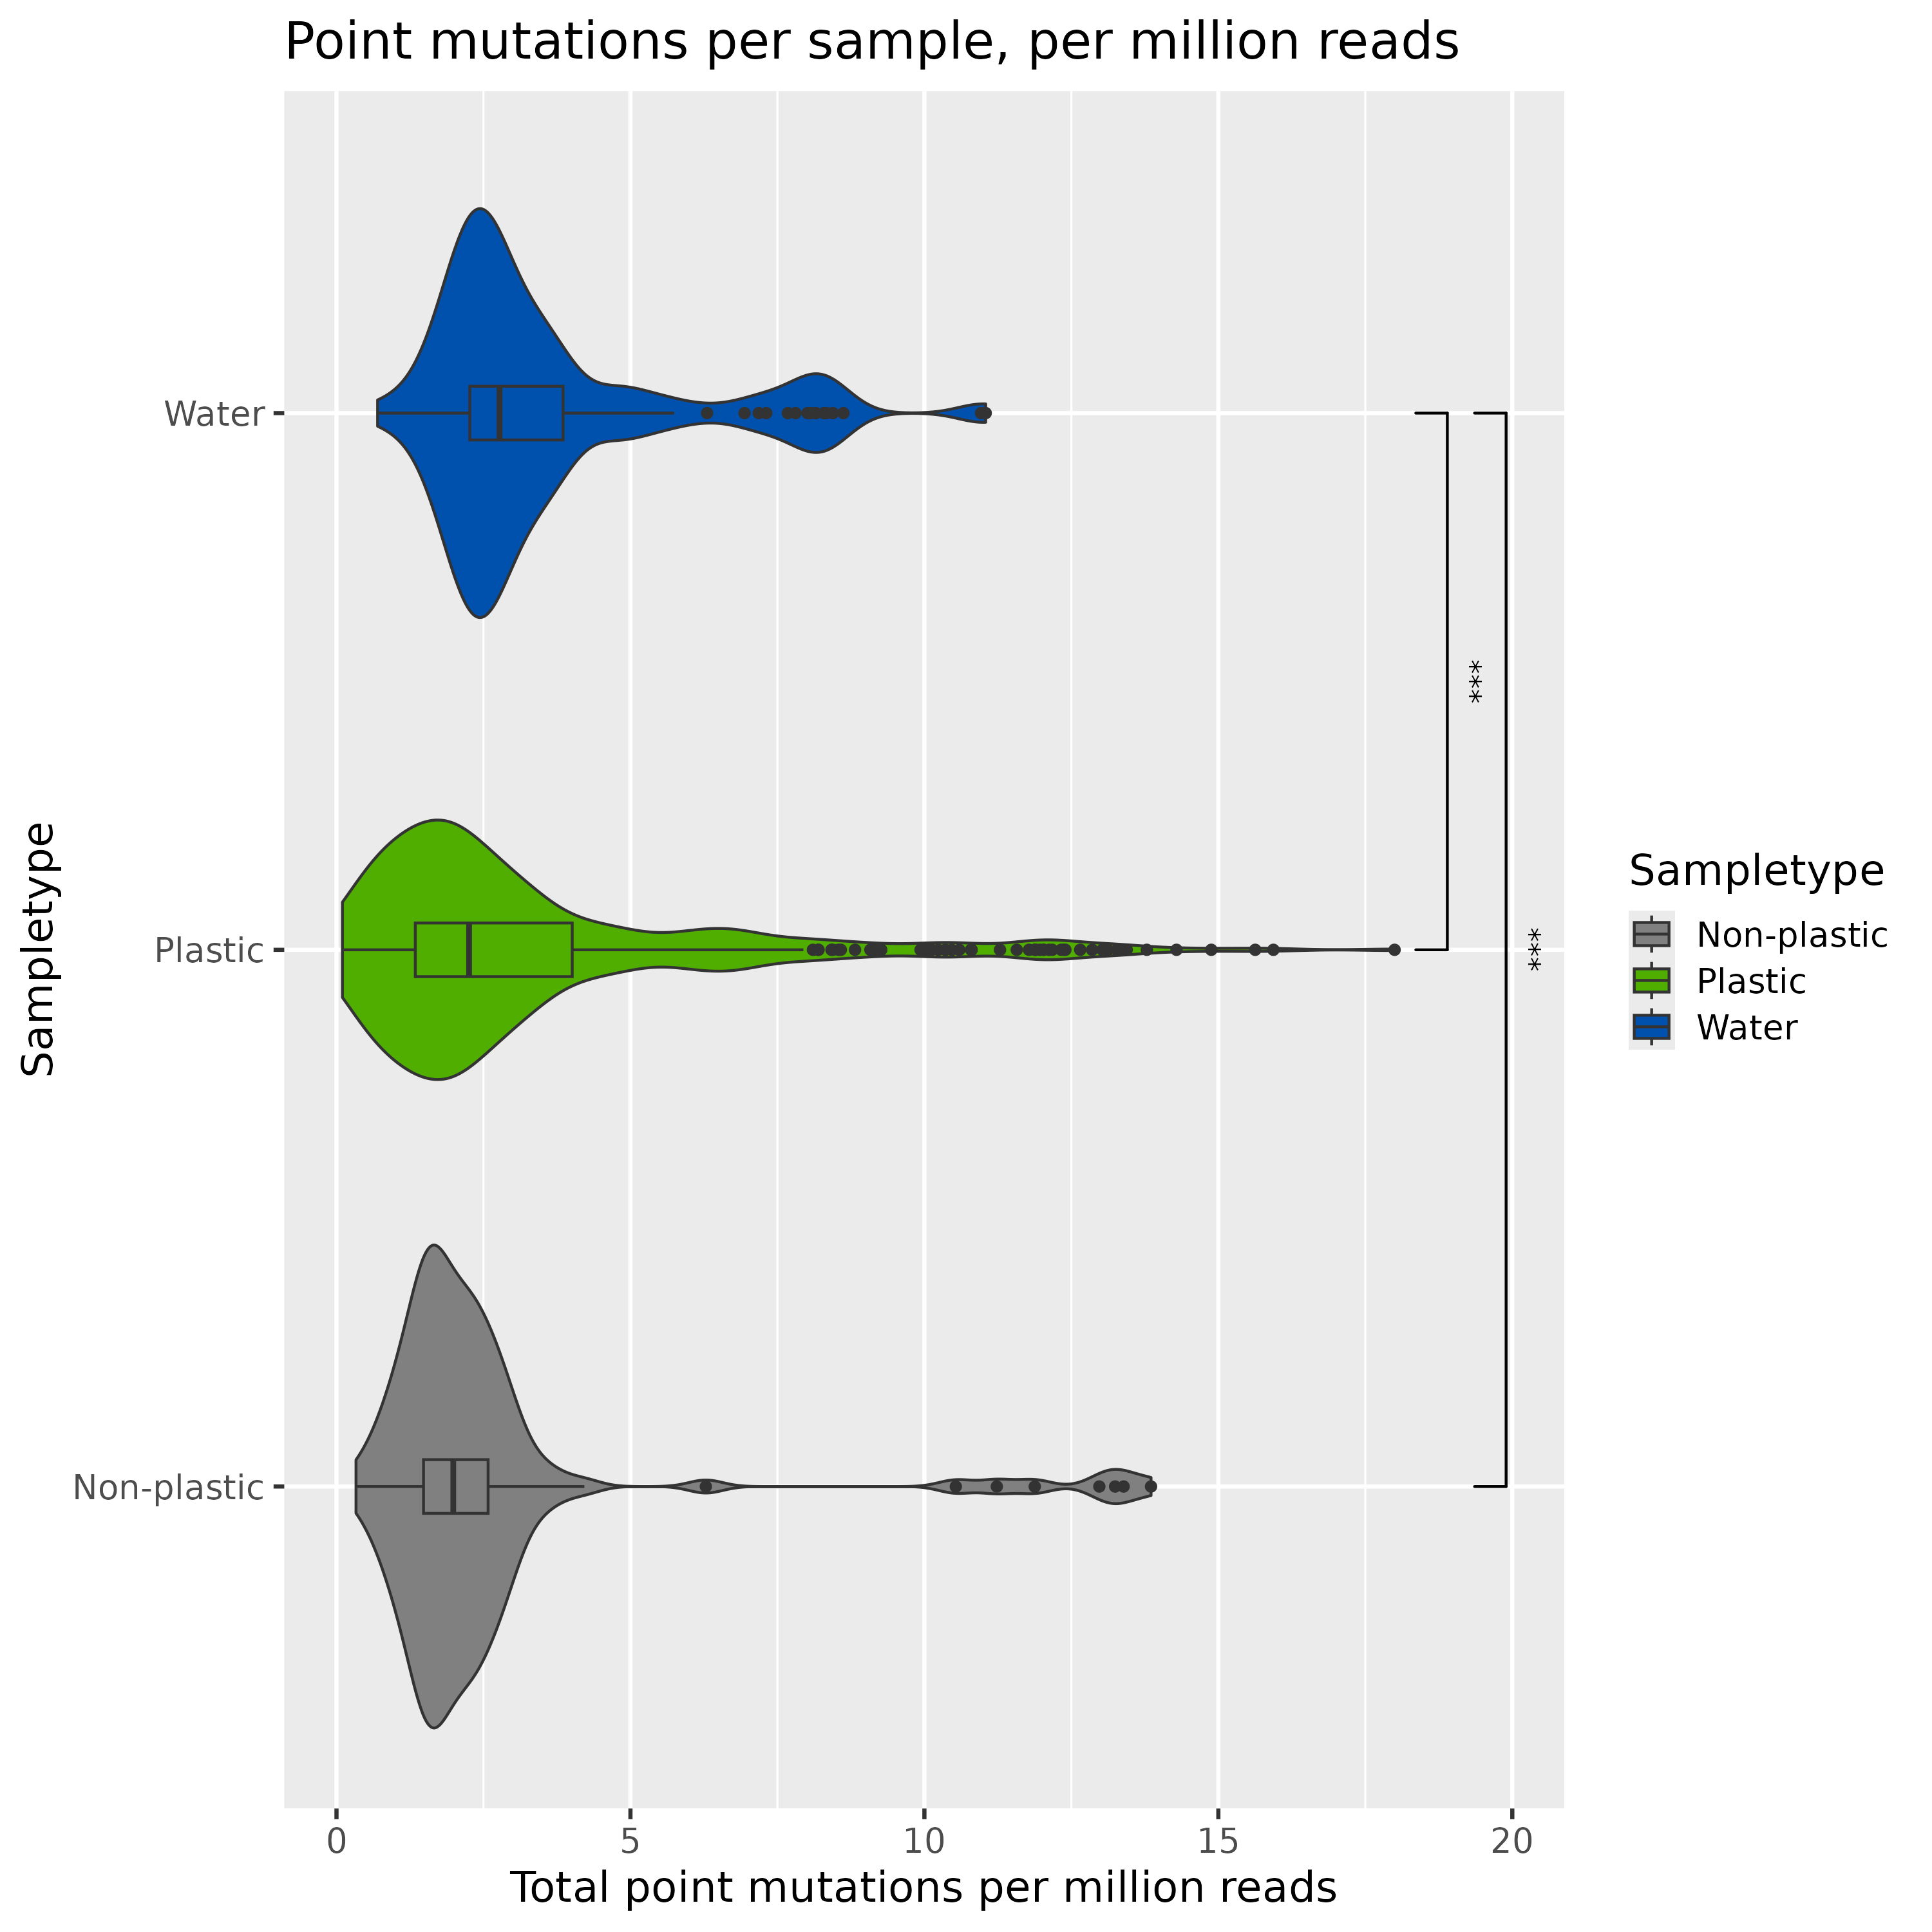
\includegraphics[width = 0.75\textwidth]{figure/hits_per_million_type.png}
    \caption{Total number of mutations per sample, grouped by sampletype. *** = p < 0.001}
    \label{hits_type}
\end{figure}

%There are also differences when comparing between different substrate types in the same way, as shown in figure \ref{hits_substrate}. The significance of these comparisons are shown in \ref{wilcox_hits_substrate}.
There are differences between the total number of point mutations for different substrate types when the total point mutations are compared, as shown in figure \ref{hits_substrate}, where the significance of these comparisons are shown in \ref{wilcox_hits_substrate}.
The plastic substrates PE-fiber-PE (PFP), Ecovio, and BI-OPL show an increase (p < 0.05) in the number of point mutations compared to most other substrates. Both Ecovio and BI-OPL are biodegradable plastics, while PFP is not.
High-density polyethylene (HDPE) show a significant (p < 0.05) decrease in the number of point mutations compared to all other substrates.
%The result of grouping the samples by substrate type instead is shown in figure \ref{hits_substrate}, which show that there was a great difference in total hit count per million between different substrate types. 
%Figure \ref{wilcox_hits_substrate} show the statistical significance of the comparison, where a wilcoxon test was done for the Substrate versus the Reference. The figure also shows the sign of the pseudo-mean for the comparison, labelled "Change", and is set to Increase if the pseudo-mean is positive and Decrease if it negative.
%Note that all comparisons were done, but only the significant ones (p < 0.05) are shown.
%There are some plastic substrates which increased comp ared to most other substrates. These include PFP, Ecovio and BI-OPL. 
The plastic substrates which show a significant increase compared to any of the water substrates are polyhydroxybutyrate (PHB), PE-fiber (PF), polybutylene adipate terephthalate (PBAT), low-density polyethylene (LDPE), Ecovio, and BI-OPL.
The soil substrate also show an overall increase in point-mutation rates compared to most other substrates, as does freshwater and seawater, with the exception of PFP, Ecovio, and BI-OPL. 

% Based on the result in these figures, it is evident that the number of point mutations which confer antibiotic resistance are not more prevalent on all plastics, but instead that specific plastic substrates increase this count.
% These substrates include PFP, Ecovio, and BI-OPL. The latter two are biodegradable plastics which contain a blend of PBAT and PLA. 


\begin{figure}[h!]
    \centering
    \subfloat[\label{hits_substrate}]{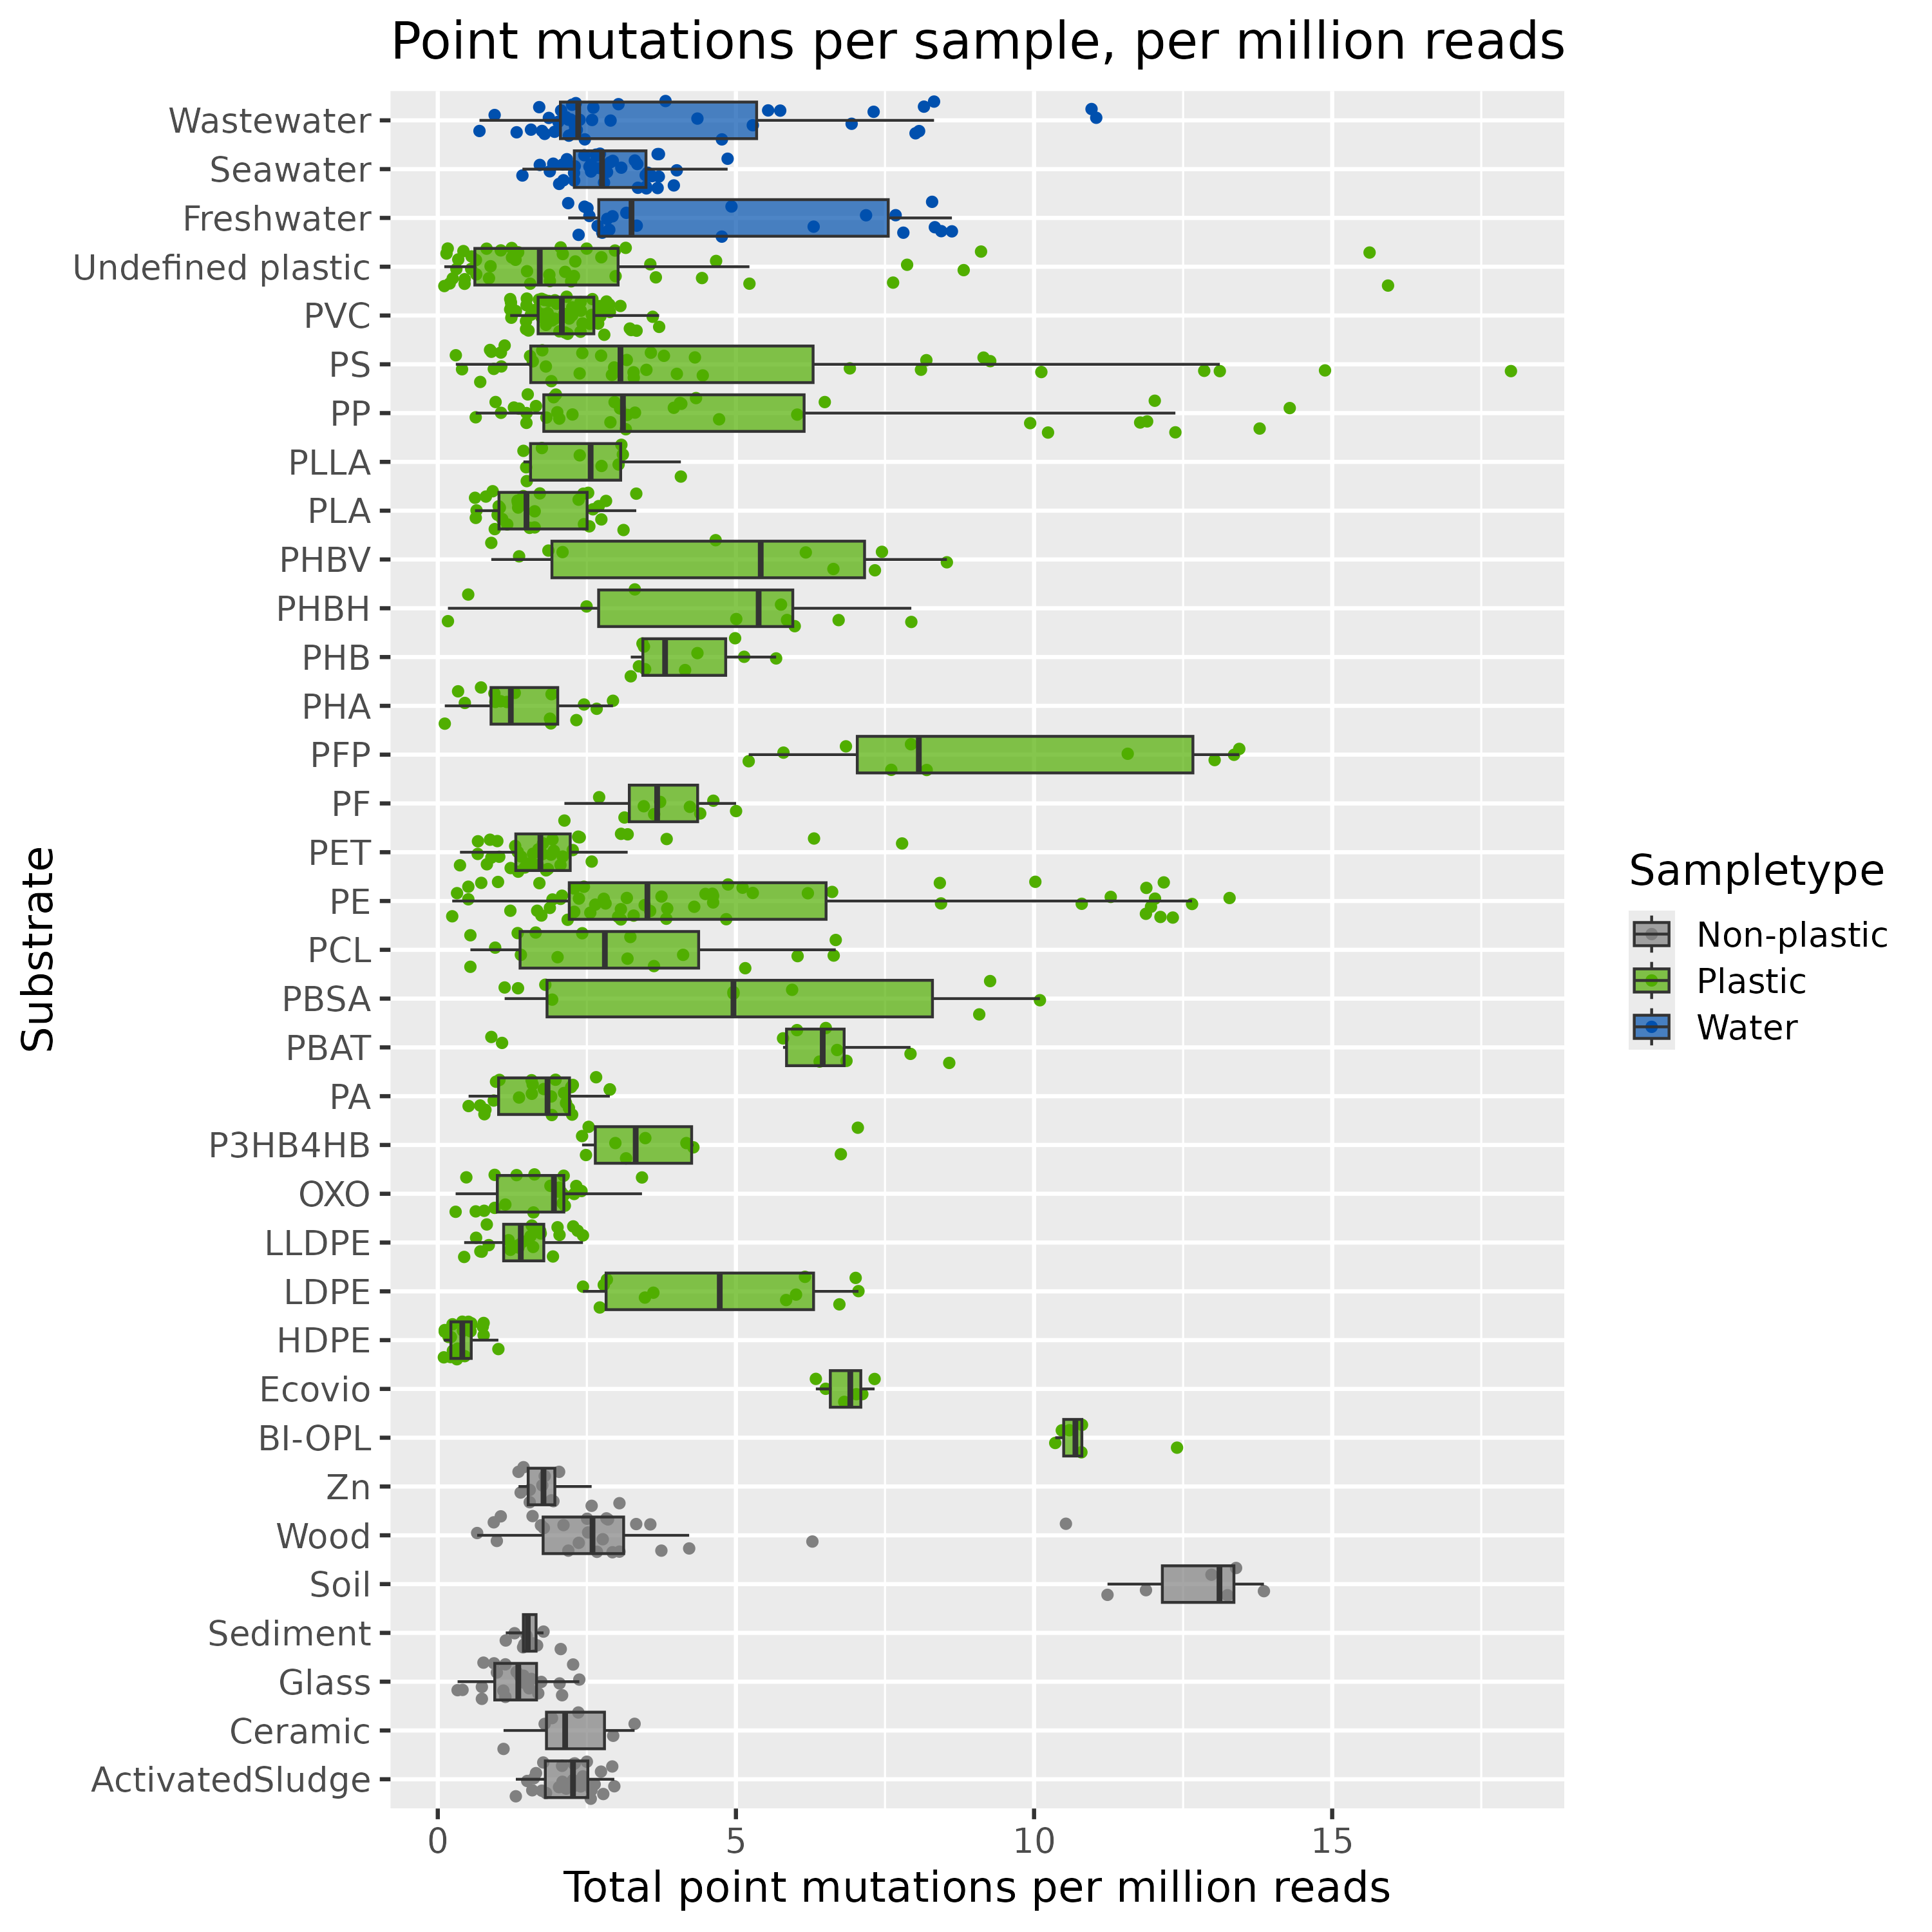
\includegraphics[width=0.5\textwidth]{figure/hits_per_million_substrate.png}}
    \subfloat[\label{wilcox_hits_substrate}]{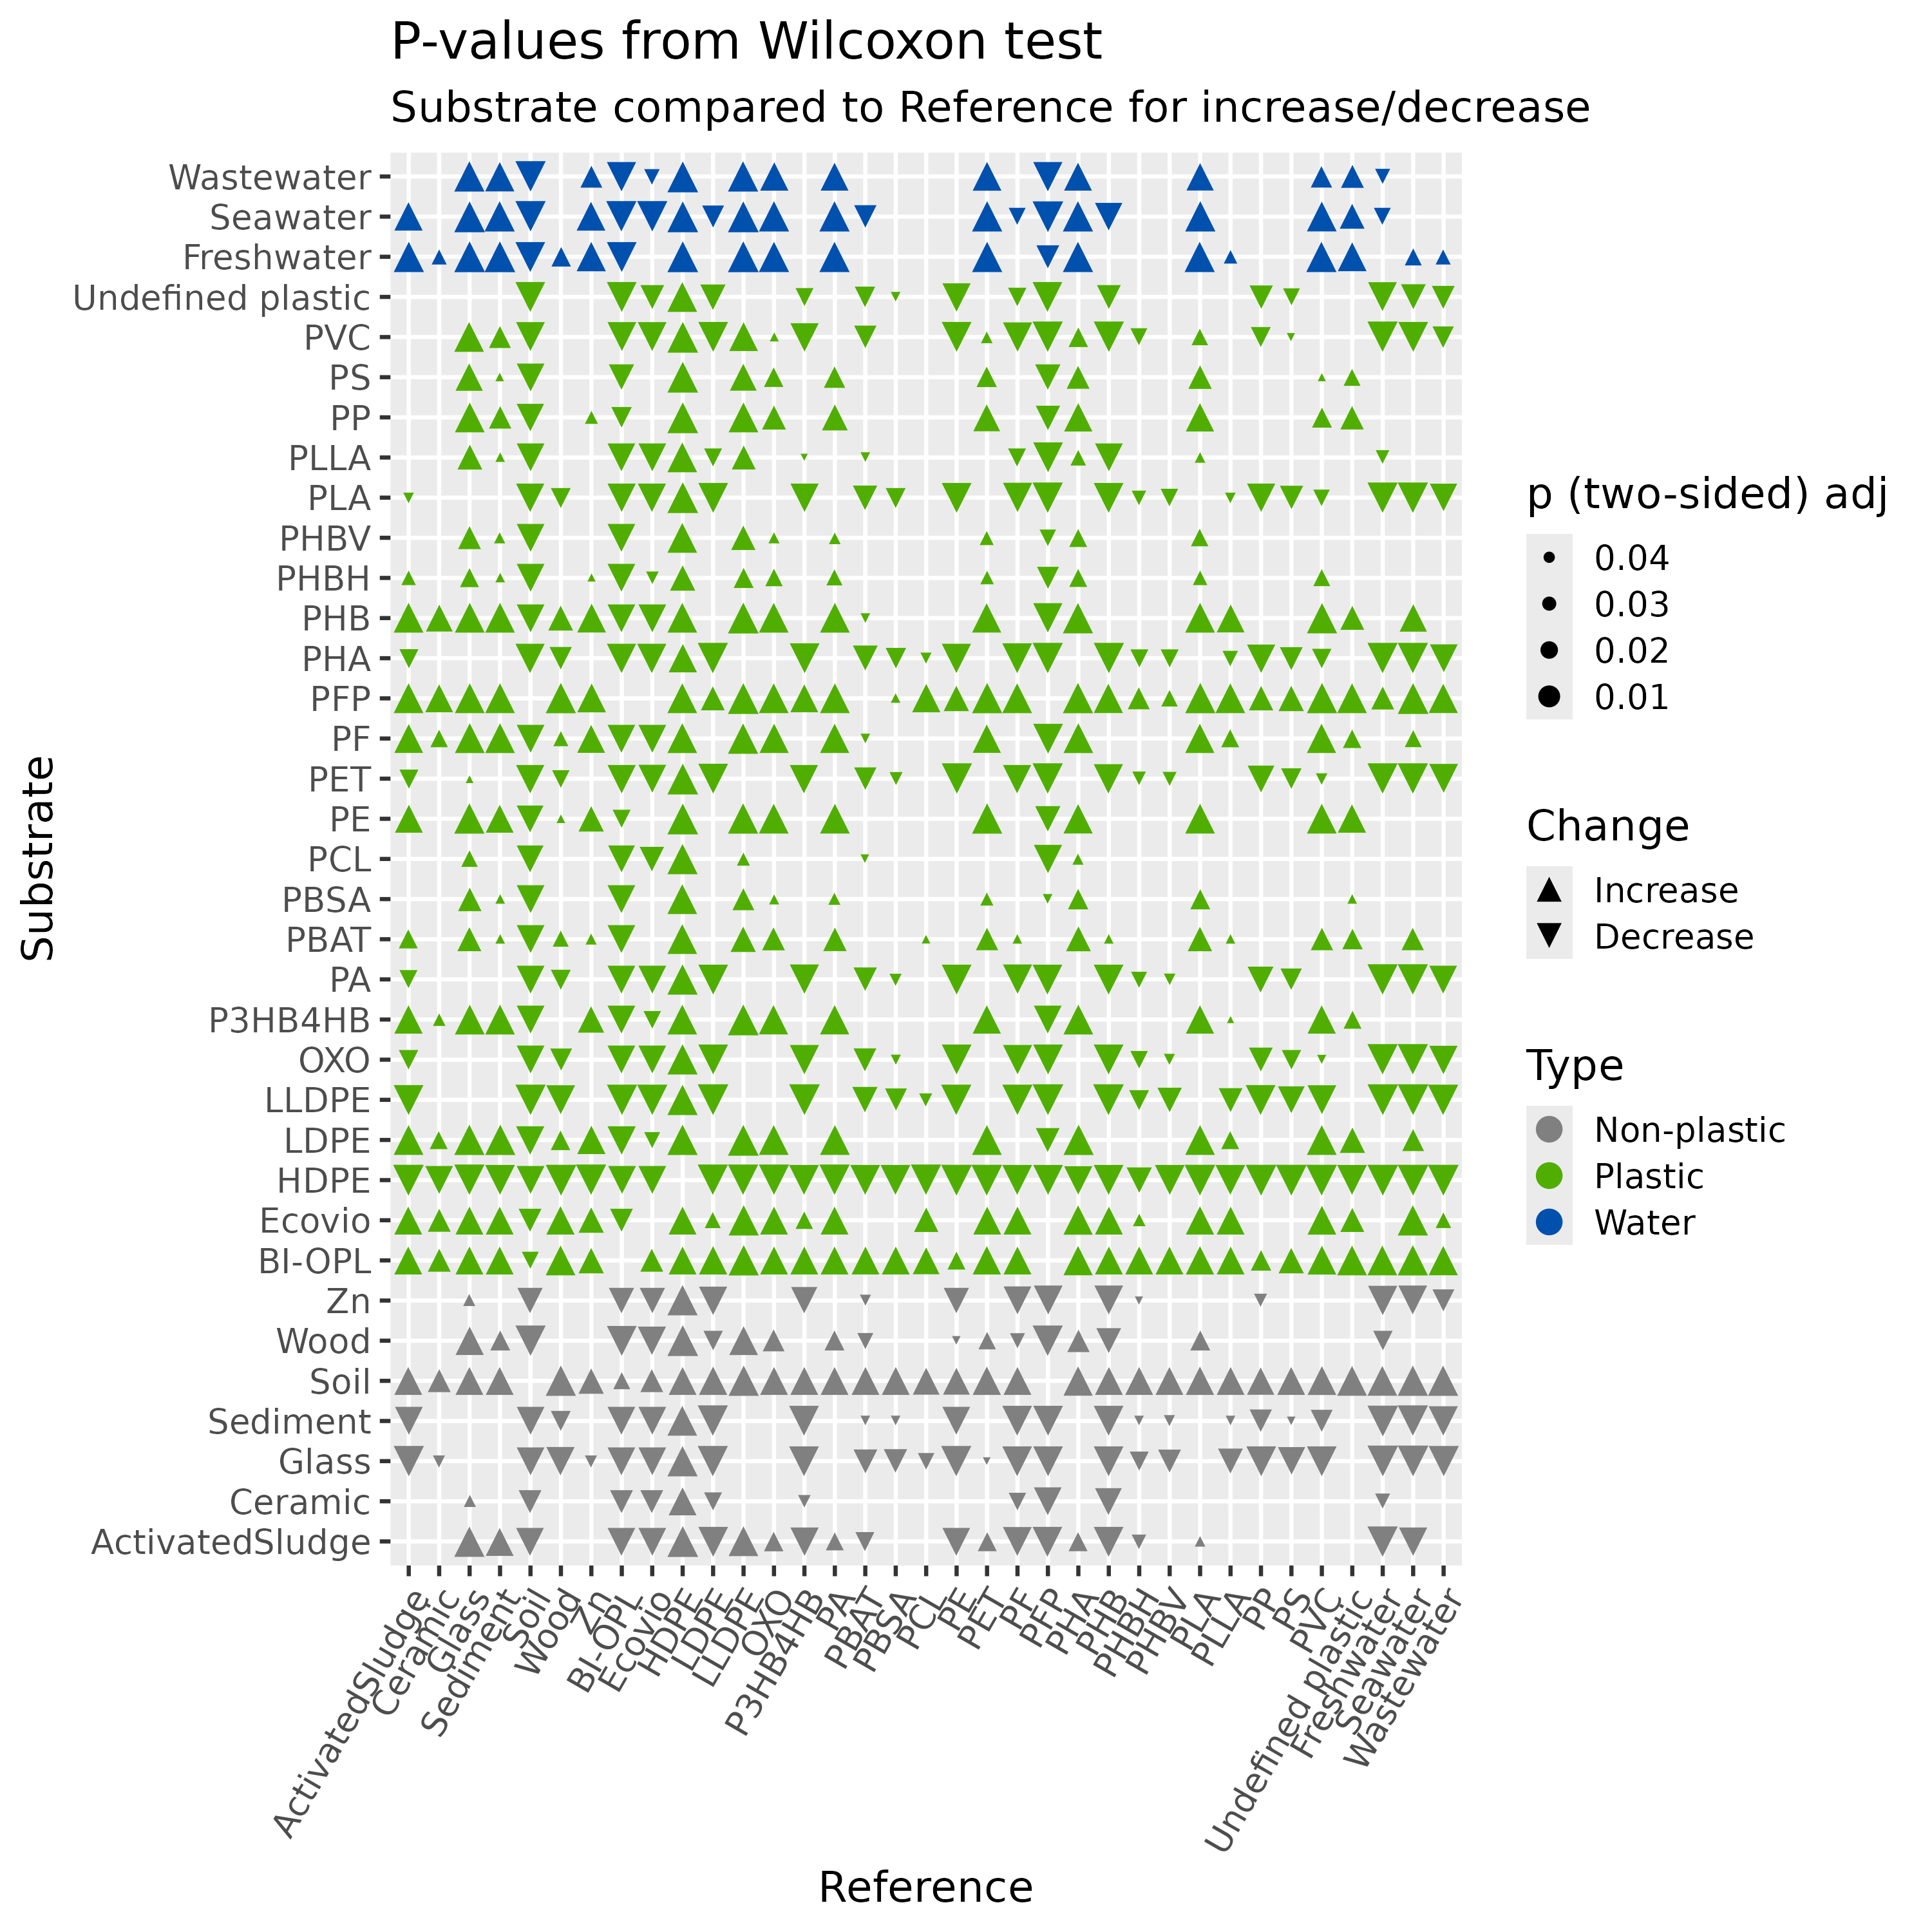
\includegraphics[width=0.5\textwidth]{figure/wilcox_hits_substrates.png}}
    \caption{(a) Point mutations per million reads. (b) p-values from Wilcoxon test for the number of point mutations of Subtrate versus Reference}
    \label{both_hits_substrate}
\end{figure}


\section{Mean mutation percentage}
%todo{Mention how the samples are collected, that they take the biofilm and sequence that? Check in a study what they do}
The following section present the results of using the mean mutation percentage instead of the total number of point mutations, which has the advantage of reducing the impact of genes which a large number of reads map to, instead using the relative mutation frequency of each individual gene.
As described above this mean value can be calculated for either the samples or the mutations. These values tell you different things, where in the first case it estimates how mutated the genes are in the samples, i.e. "this sample has a mean mutation percentage of 3\%".
In the latter case it estimates how mutated specific genes are in the different substrates, i.e. "mutation A has a mean mutation percentage of 25\% in freshwater" \todo{Same problem as in Method, how to describe it.}.
% The advantage of this approach is that the relative mutation frequency of the gene is used instead of the total number of point mutations, which normalizes the mutation rate and reduces the impact of genes which a large number of reads map to.

%\subsection{Mean mutation percentage of samples} 
%\subsubsection{Alternative 1, combined plots, otherwise two separate larger plots, see \ref{mean_samples_substrate_full} and \ref{wilcox_samples_substrates_full}}
%The mean mutation percentage was calculated for every sample, and 
Figure \ref{mean_samples_sampletype} show the mean mutation percent grouped by the type of sample.
There is a significant difference (Wilcoxon test: p < 0.001) between the water group and the plastic group, where the plastic group has a lower mean mutation percentage in comparison to the water group. None of the other groups displayed any significant difference (p < 0.05) between them.

%\todo{Remove n.s.?}
\begin{figure}[h!]
    \centering
    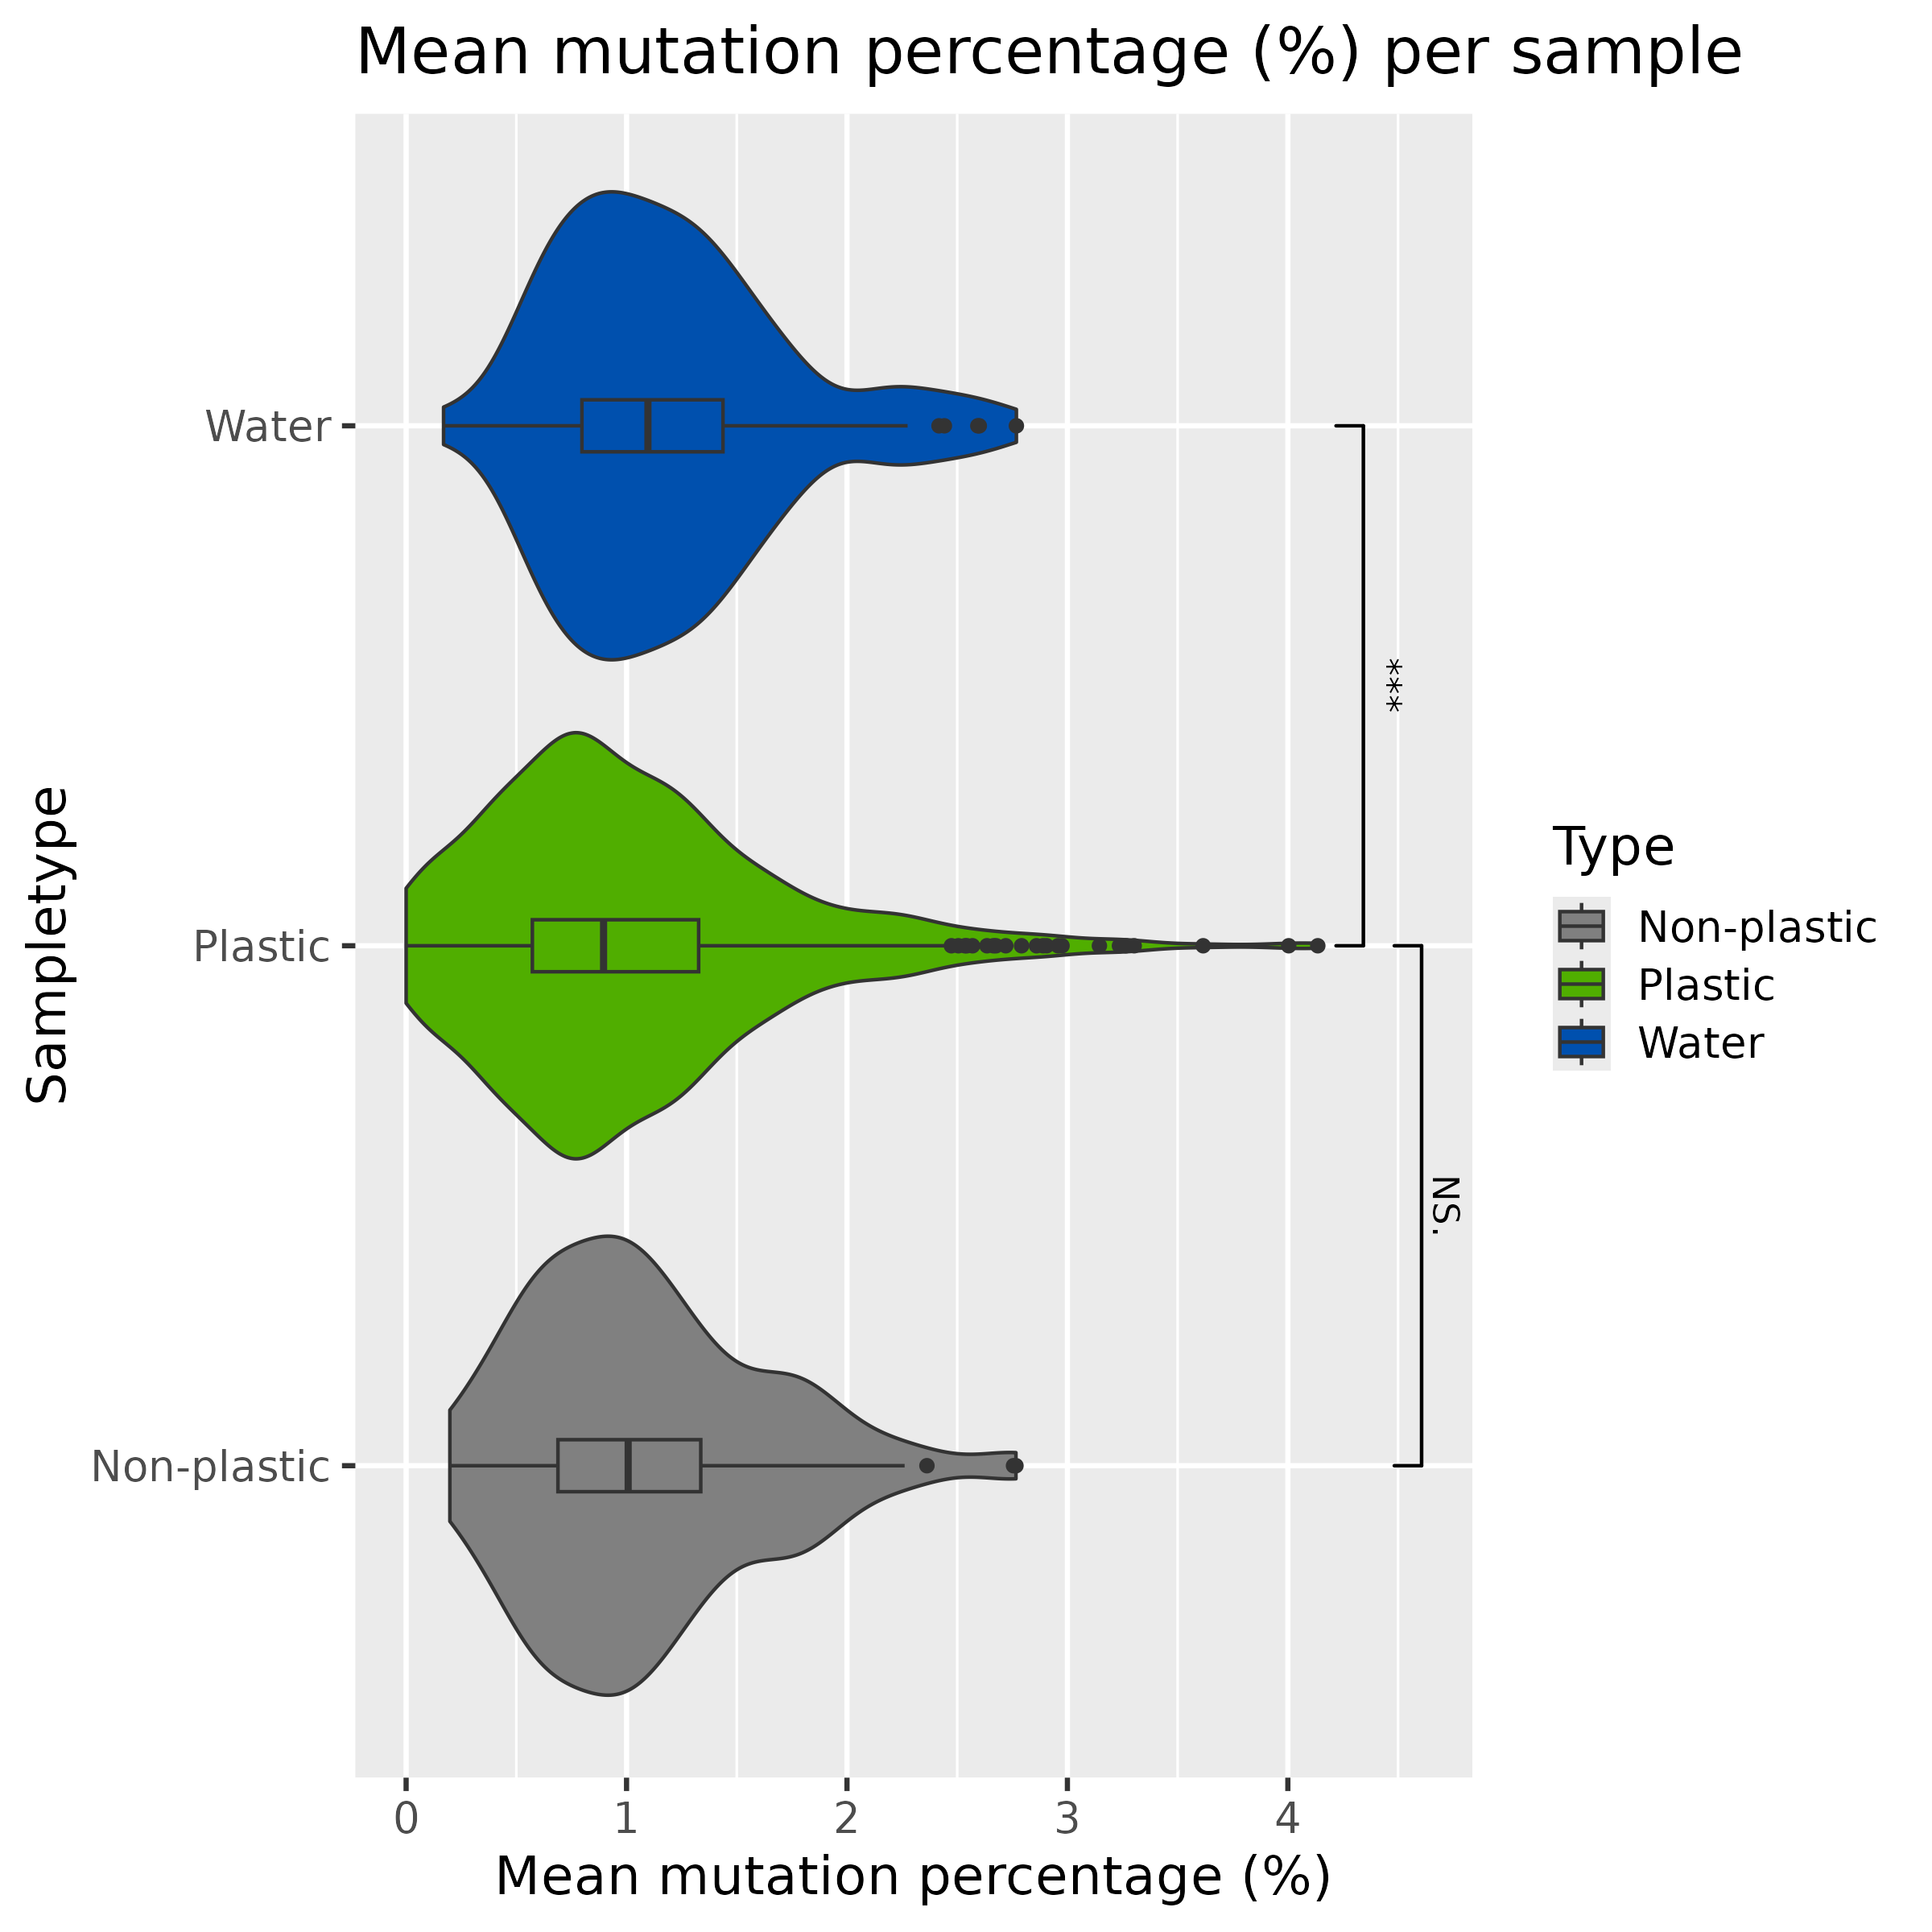
\includegraphics[width = 0.6\textwidth]{figure/mean_samples_sampletype.png}
    \caption{Mean mutation percentage (\%) per sample, grouped by sampletype. * = p < 0.05, *** = p < 0.001}
    \label{mean_samples_sampletype}
\end{figure}
%\todo{P-values-table in appendix or not at all?)}

% \begin{table}[h]
% \caption{p-values from Wilcoxon test between sampletypes}
% \label{wilcox_samples_sampletype}
% \begin{tabular}{@{}llllll@{}}
% \toprule
% Sampletype A & Sampletype B & Significance & Change   & p (two-sided) & pseudo\_mean  \\ \midrule
% Non-plastic  & Plastic      & *            & Increase & 0.0473  &  0.0012  \\
% Water        & Plastic      & ***          & Increase & 0.0005  &  0.0020  \\
% Non-plastic  & Water        & ns           & Decrease & 0.1801  & -0.0009 \\
% Plastic      & Water        & ***          & Decrease & 0.0005  & -0.0020 \\
% Plastic      & Non-plastic  & *            & Decrease & 0.0473  & -0.0012 \\
% Water        & Non-plastic  & ns           & Increase & 0.1801  &  0.0009 \\ \bottomrule
% \end{tabular}
% \end{table}


In figure \ref{mean_samples_substrate} the samples are instead grouped by substrate type, which shows that there are differences for different plastics, as well as other substrates.
Figure \ref{wilcox_samples_substrate} show the statistical significance of the comparison, when a Wilcoxon test was done for the Substrate versus the Reference, as well as if there is an increase of the pseudo-mean compared to the reference.
Note that all comparisons were done, but only the significant ones (p < 0.05) are shown.
There are some plastics that has a significant, higher, mean mutation percentage than most other substrates. These include PFP, LDPE, Ecovio and BI-OPL. The last two plastics are biodegradable plastics.
The plastic substrates that has a significant higher mean mutation percentage than seawater or wastewater include polyvinyl chloride (PVC) and PF in addition to PFP, LDPE, Ecovio and BI-OPL.
There are also some plastics which have significantly different lower mean mutation percentage than almost all other substrates, the most notable of which is high-density polyethylene (HDPE), poly(3-hydroxybutyrate-co-3-hydroxyvalerate) (PHBV) and polyhydroxyalkanoate (PHA), of which the latter two are biodegradable polymers while the first one is not.
Almost all substrates have a significantly different lower mean mutation percentage than the freshwater samples and the soil samples, the exception of which is Ecovio, BI-OPL, and PFP where there is no significant (p < 0.05) difference. 
%The soil samples have a significantly higher (p < 0.001) mean mutation percentage compared to most other substrates. 
%todo{meh, "which is expected from previous studies" + ref? Idk varför det nämns}.


\begin{figure}[h!]
    \centering
    \subfloat[\label{mean_samples_substrate}]{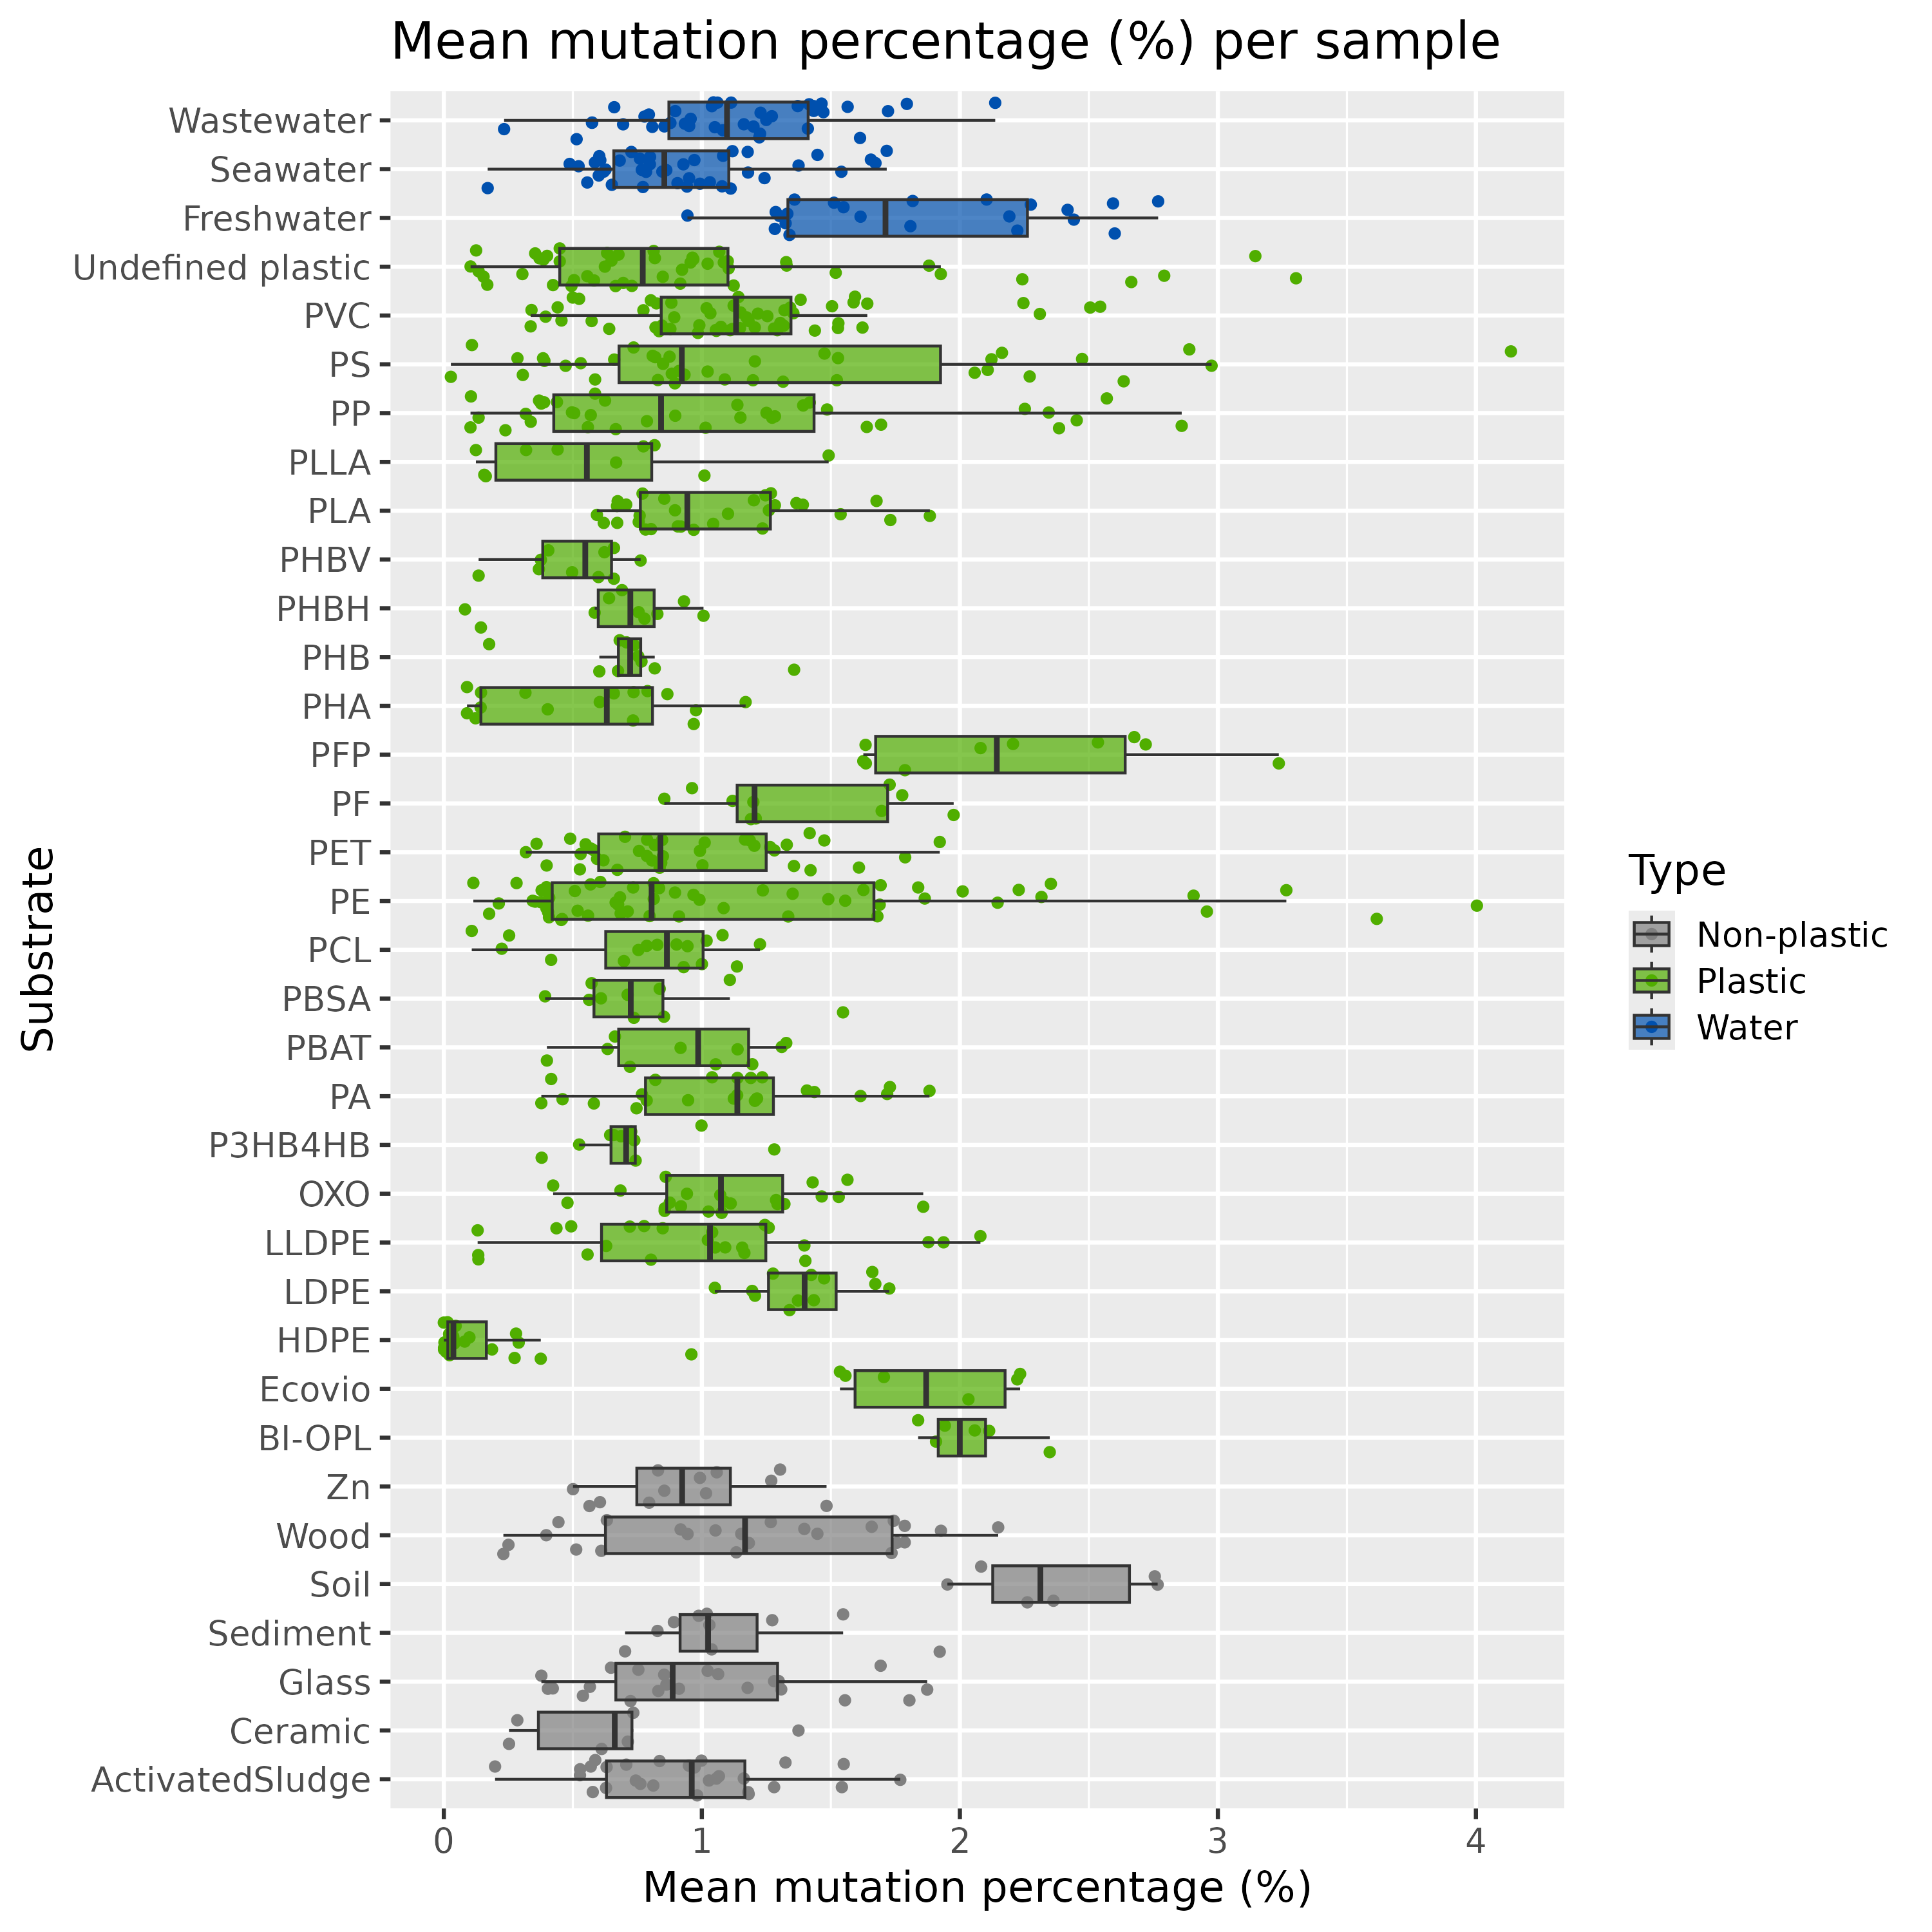
\includegraphics[width=0.5\textwidth]{figure/mean_samples_substrate.png}}
    \subfloat[\label{wilcox_samples_substrate}]{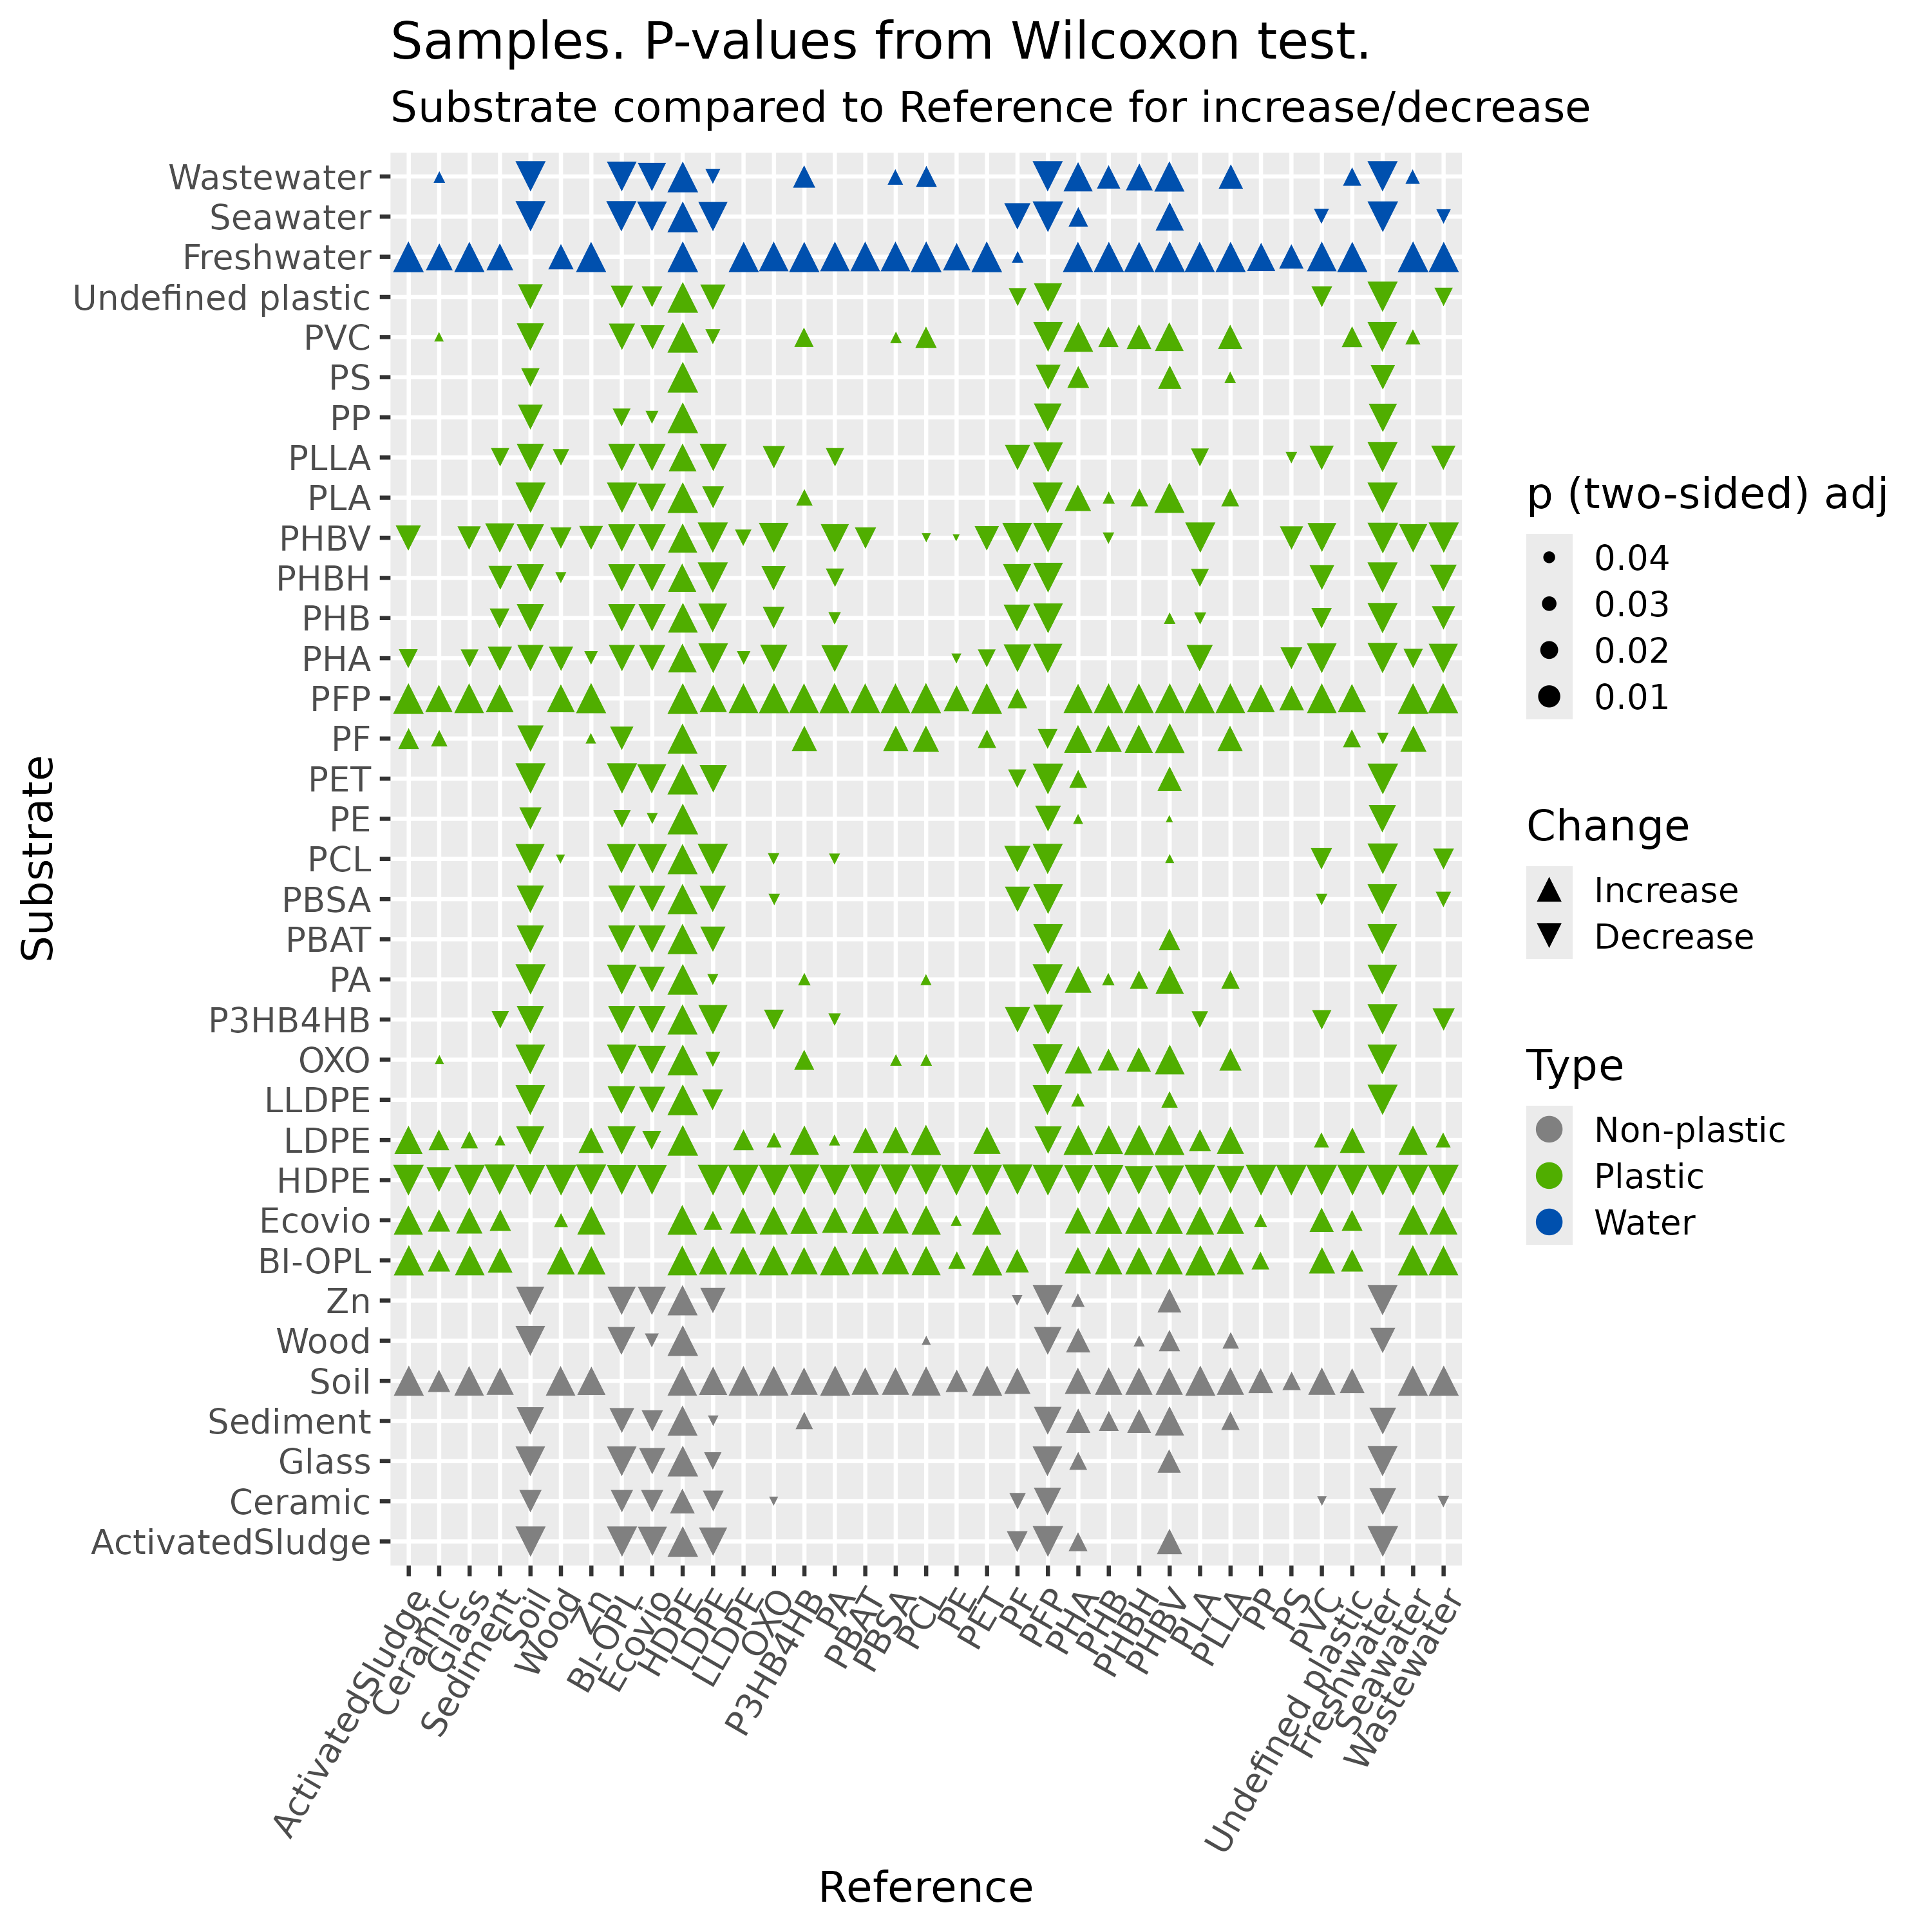
\includegraphics[width=0.5\textwidth]{figure/wilcox_samples_substrates.png}}
    \caption{(a) Mean mutation percentage per sample, grouped by substrate type. (b) p-values from Wilcoxon test of mean mutation percentage for Substrate versus Reference}
    \label{both_mean_samples_susbtrates}
\end{figure}

%\subsubsection{Alternative 2, separate plots instead of combined, see figure \ref{both_mean_samples_susbtrates}}
%\begin{figure}[h]
    % \centering
    % 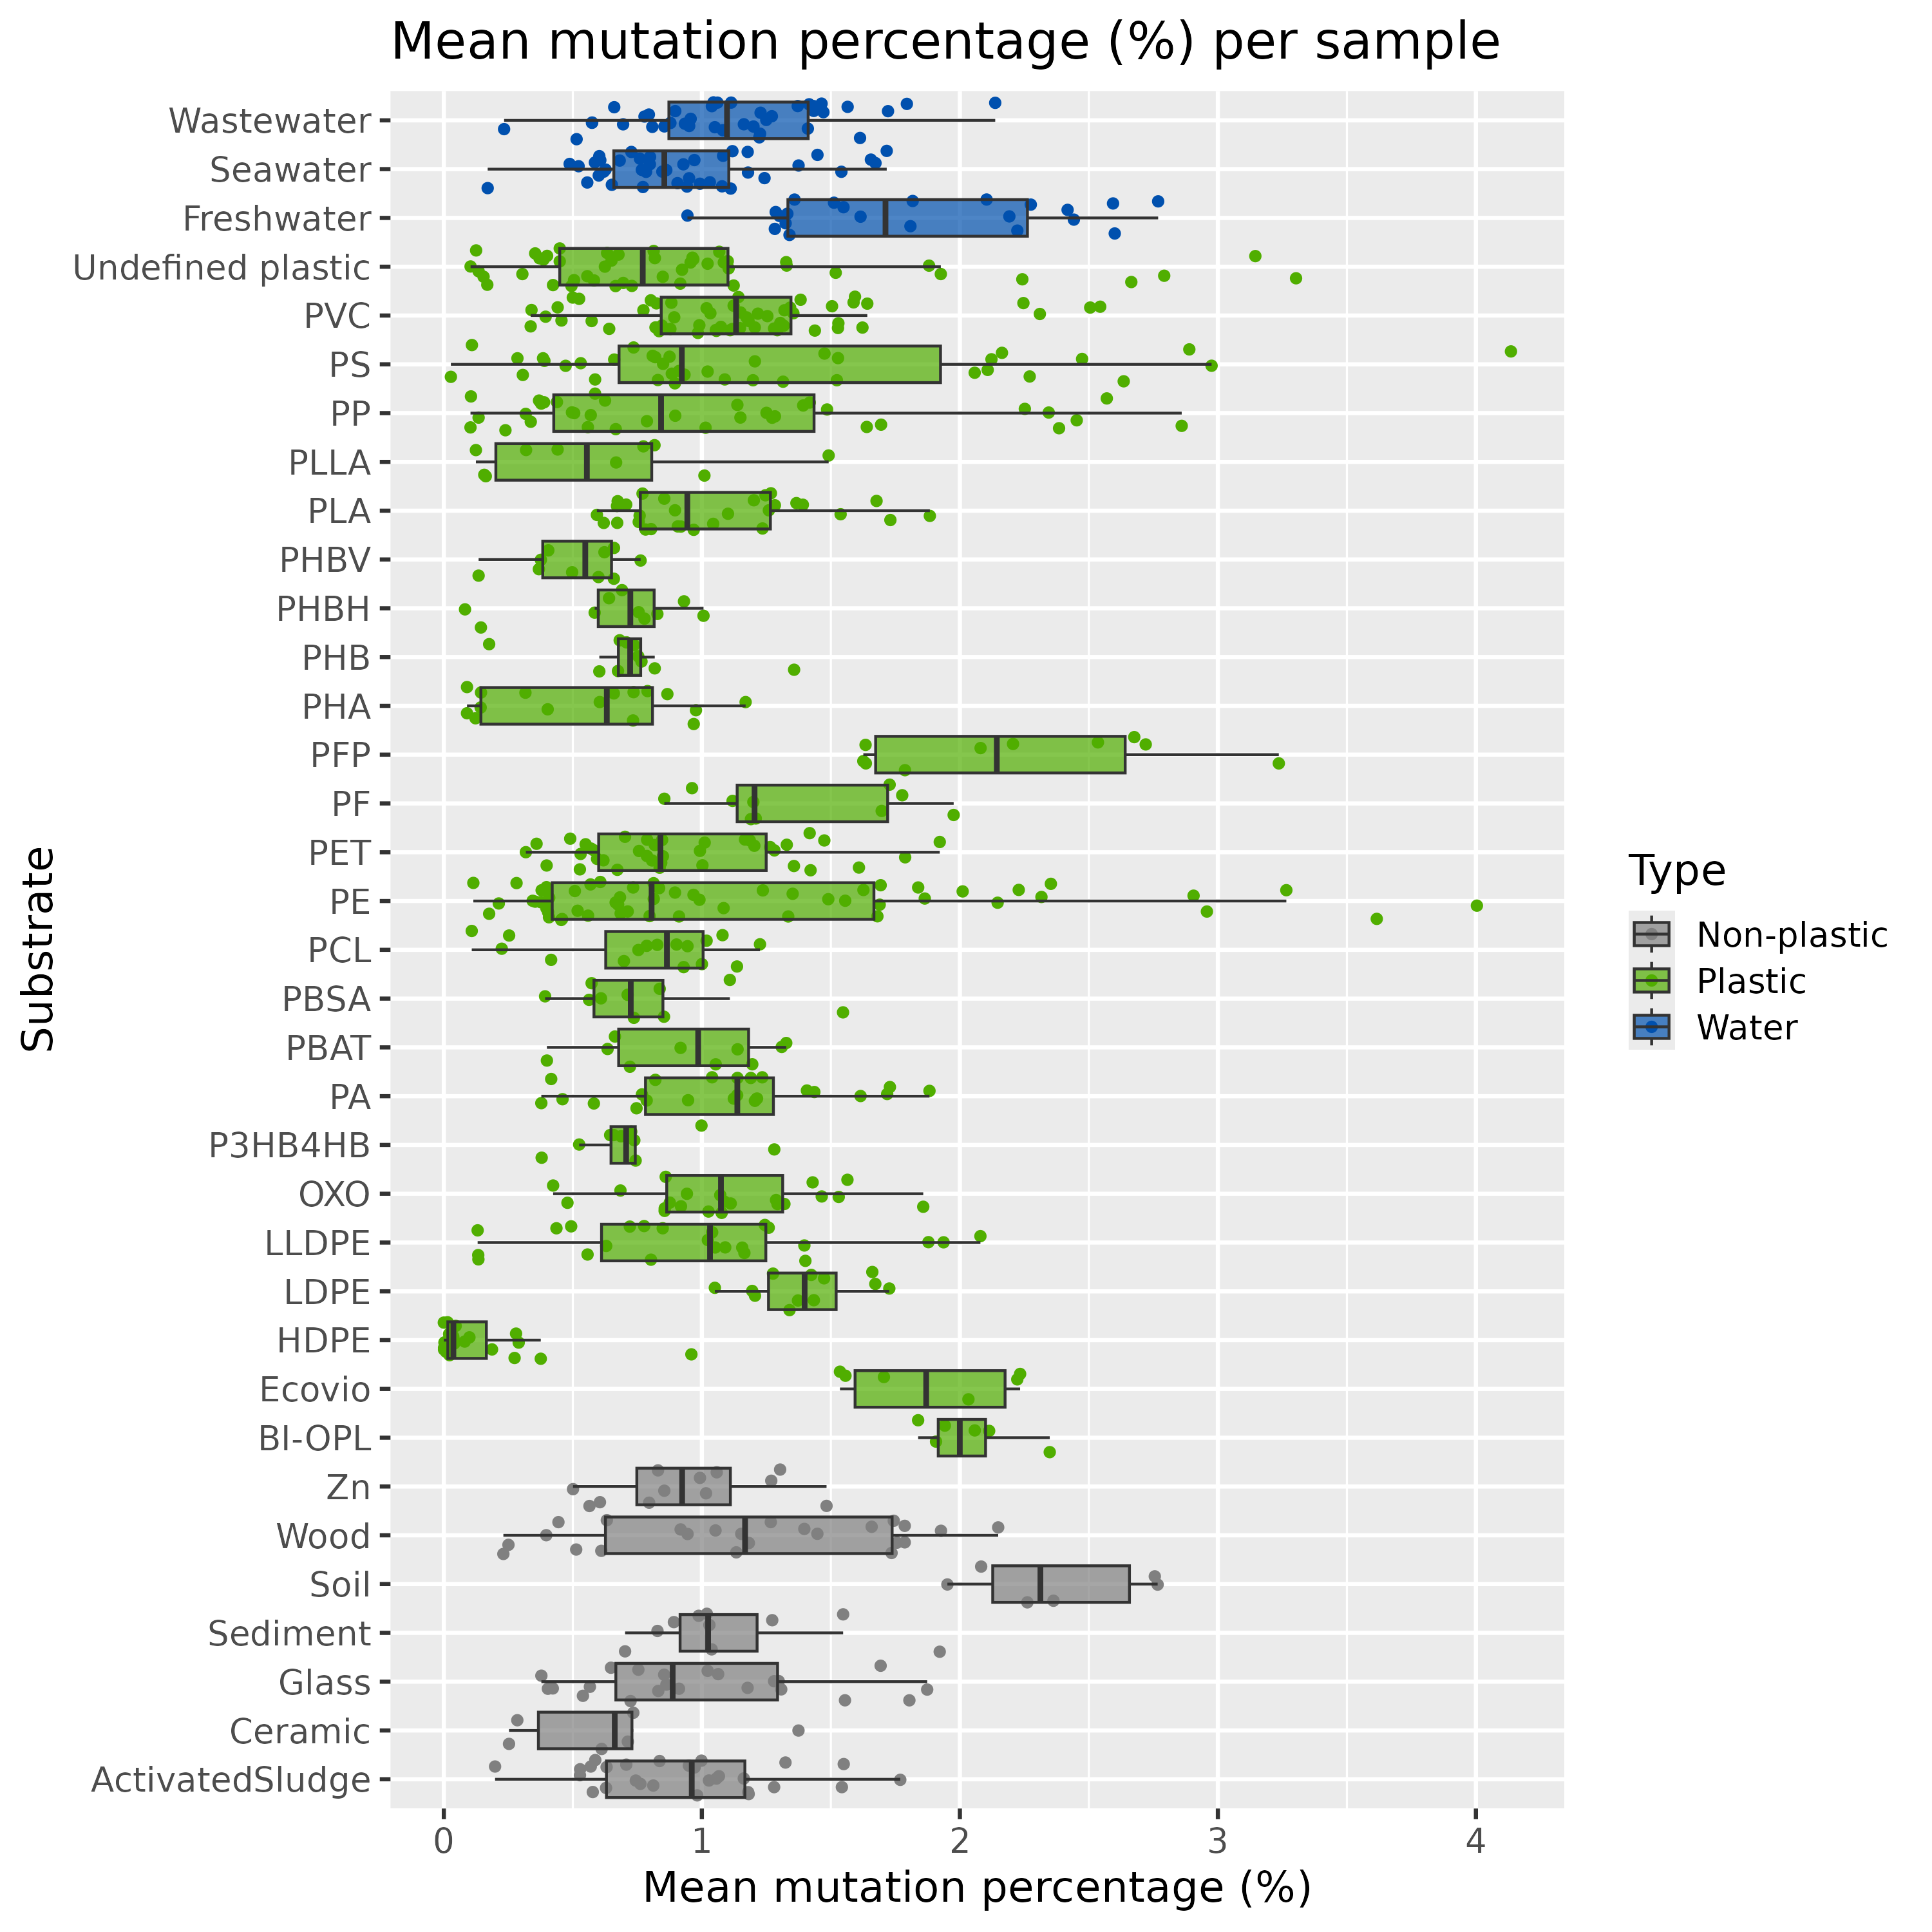
\includegraphics[width = 0.7\textwidth]{figure/mean_samples_substrate.png}
    % \caption{Mean Samples Substrate Full}
    % \label{mean_samples_substrate_full}
% \end{figure}
% 
% \begin{figure}[h]
    % \centering
    % 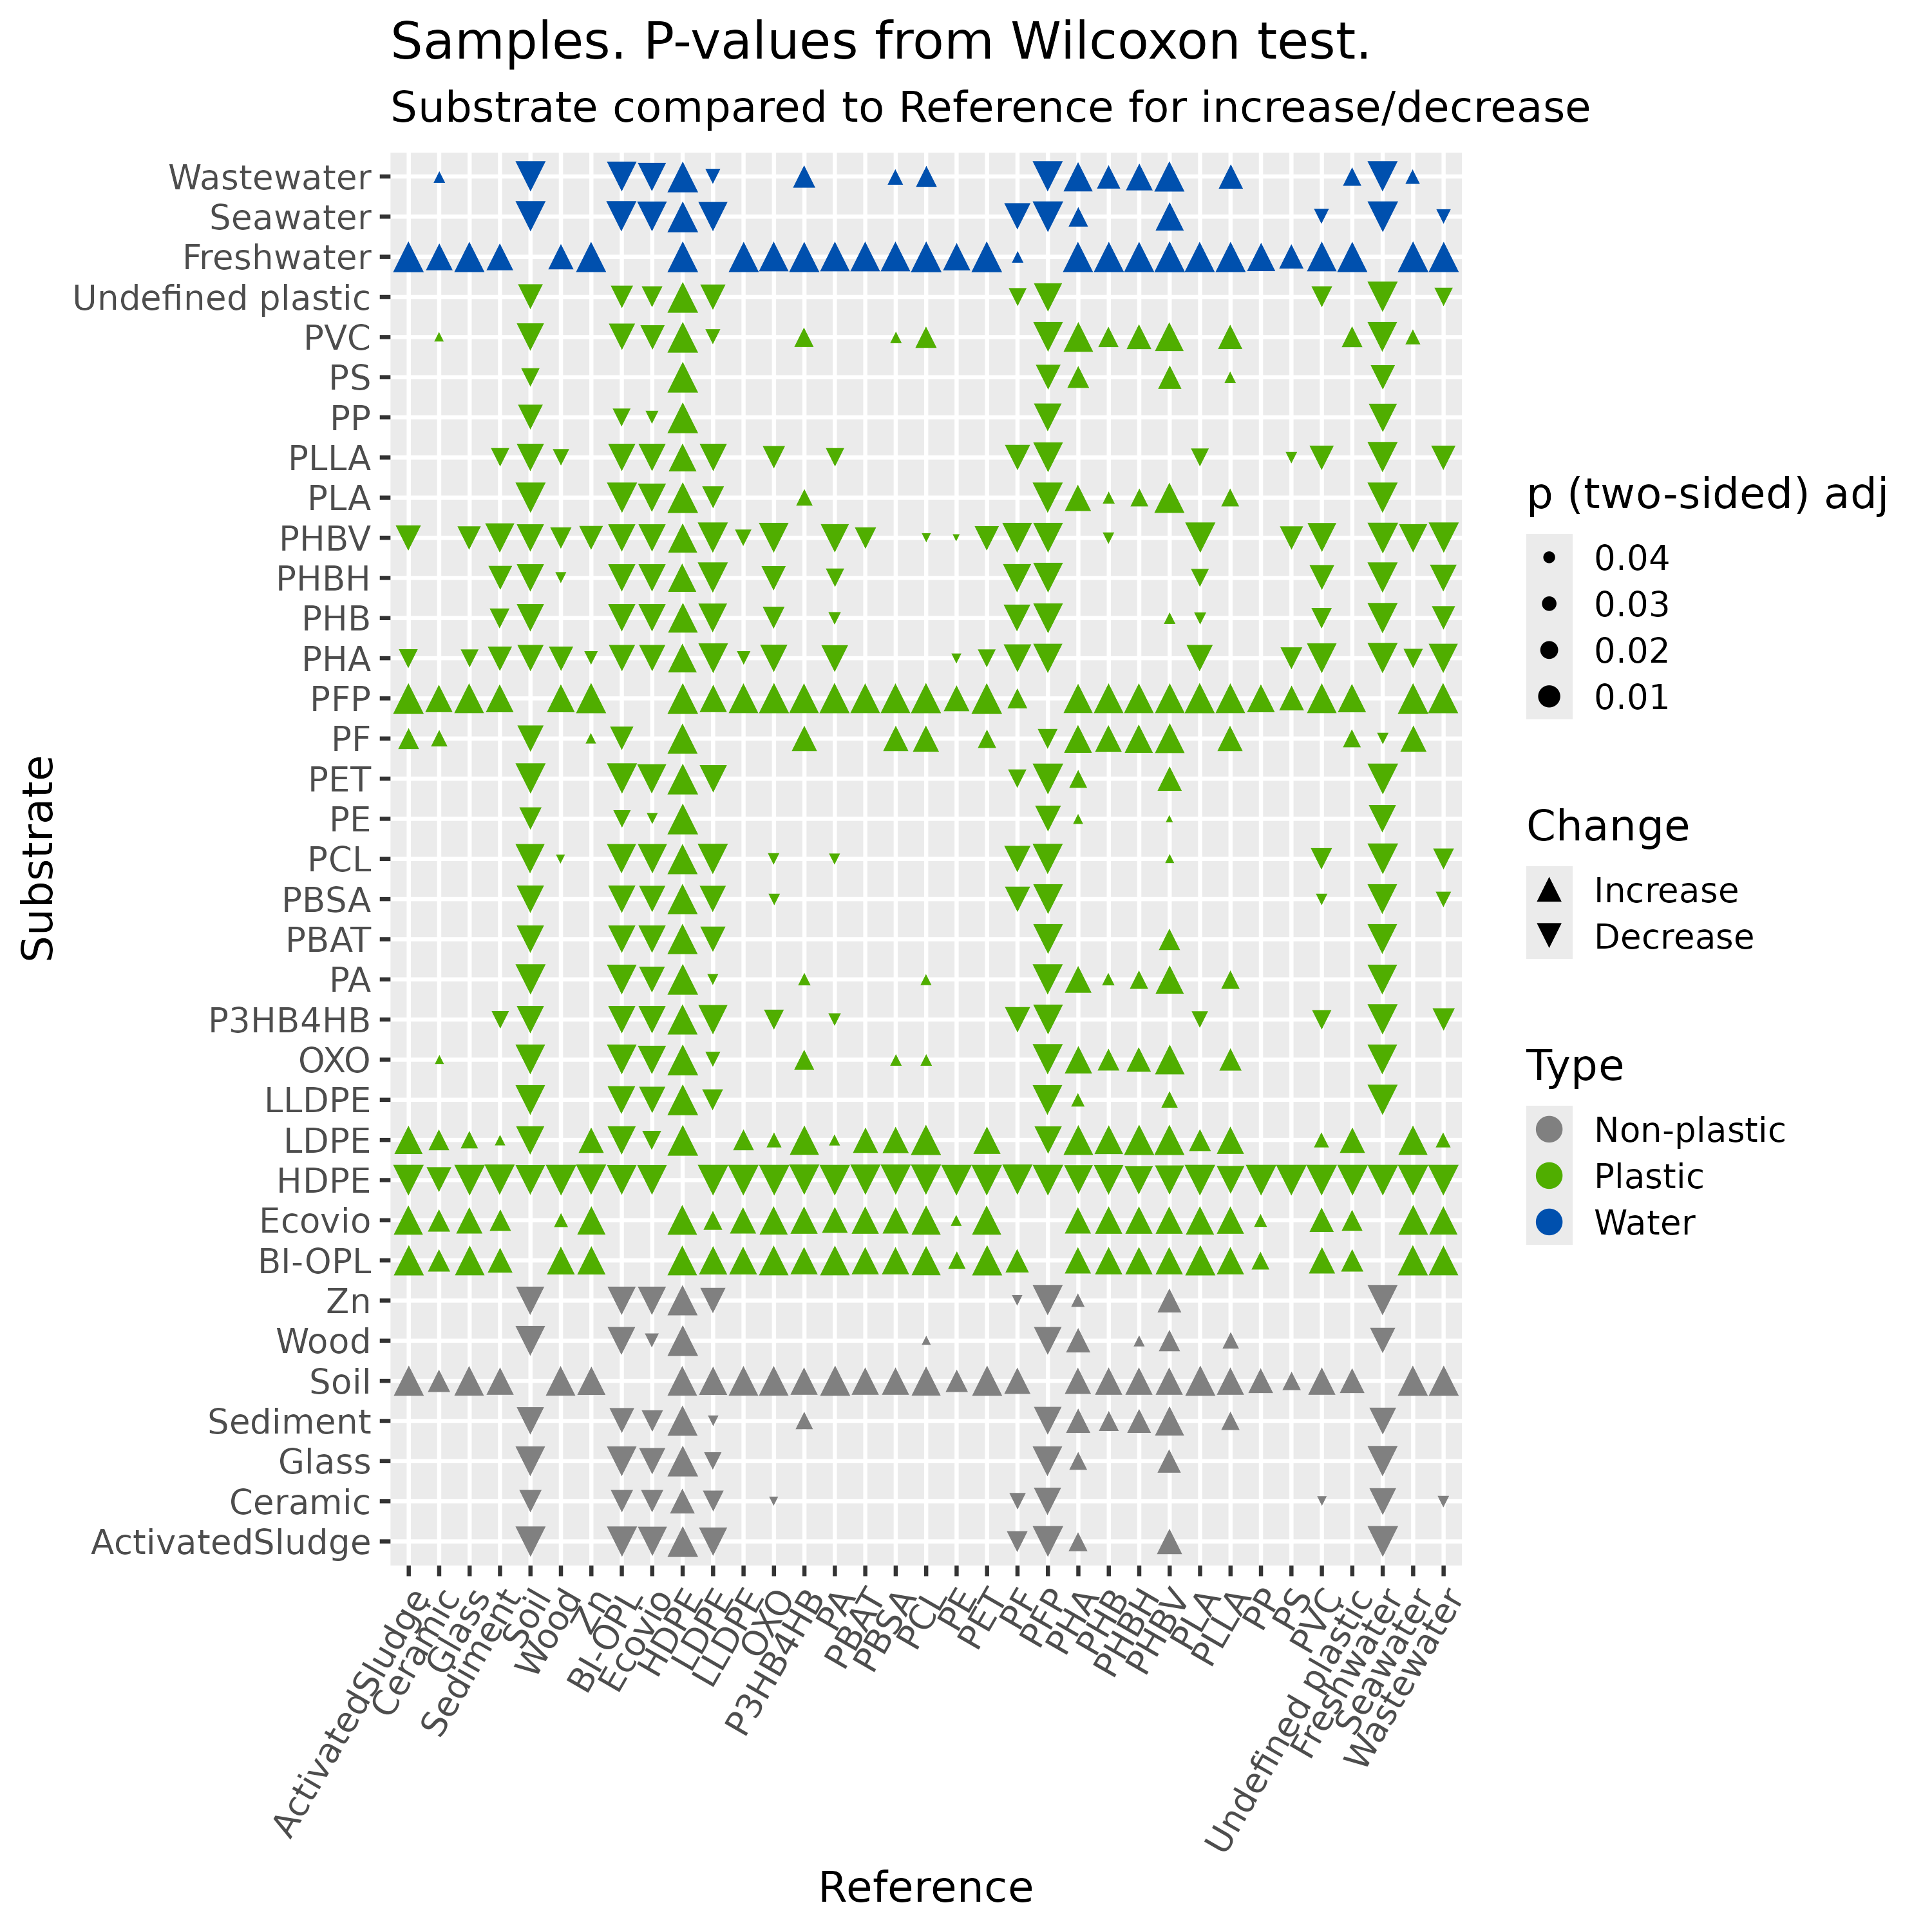
\includegraphics[width = 0.7\textwidth]{figure/wilcox_samples_substrates.png}
    % \caption{Wilcoxon Samples Substrate Full}
    % \label{wilcox_samples_substrates_full}
% \end{figure}
% 

%\subsection{Mean mutation percentage of individual mutations}
%Figure \ref{mean_genes_sampletype} show the result if instead of the mean mutation percentage for each sample was calculated, the mean mutation percentage per mutation, grouped by sampletype was calculated. \todo{i.e. mutation A12D parC for water: 10\%, A12D parC for plastic: 0\%, A12D parC for non-plastic: 3\%} 
%The resulting figure is hard to interpret since many of the genes will have a mean close to zero. If instead a log-scale was used, it removes many of the data points from the water and nonplastic groups, since they have a mean mutation percentage of zero. This skews the figure shown, and end up showing the reverse change as described below. \todo{Since we cannot use the log plot, do we need to use the bad plot instead, or can we skip it and just use stats?}
The mean mutation rate of individual point mutations grouped by sample type is shown in figure \ref{mean_genes_sampletype}. The mean mutation percentage was significantly different (p < 0.001) and higher for the plastic samples compared to both the water samples and the non-plastic samples. There is not a significant change between the water group and the non-plastic group.
% There is a significant difference between the different sample types, where plastic show an increase compared to both the water samples and the non-plastic samples.

\begin{figure}[h!]
    \centering
    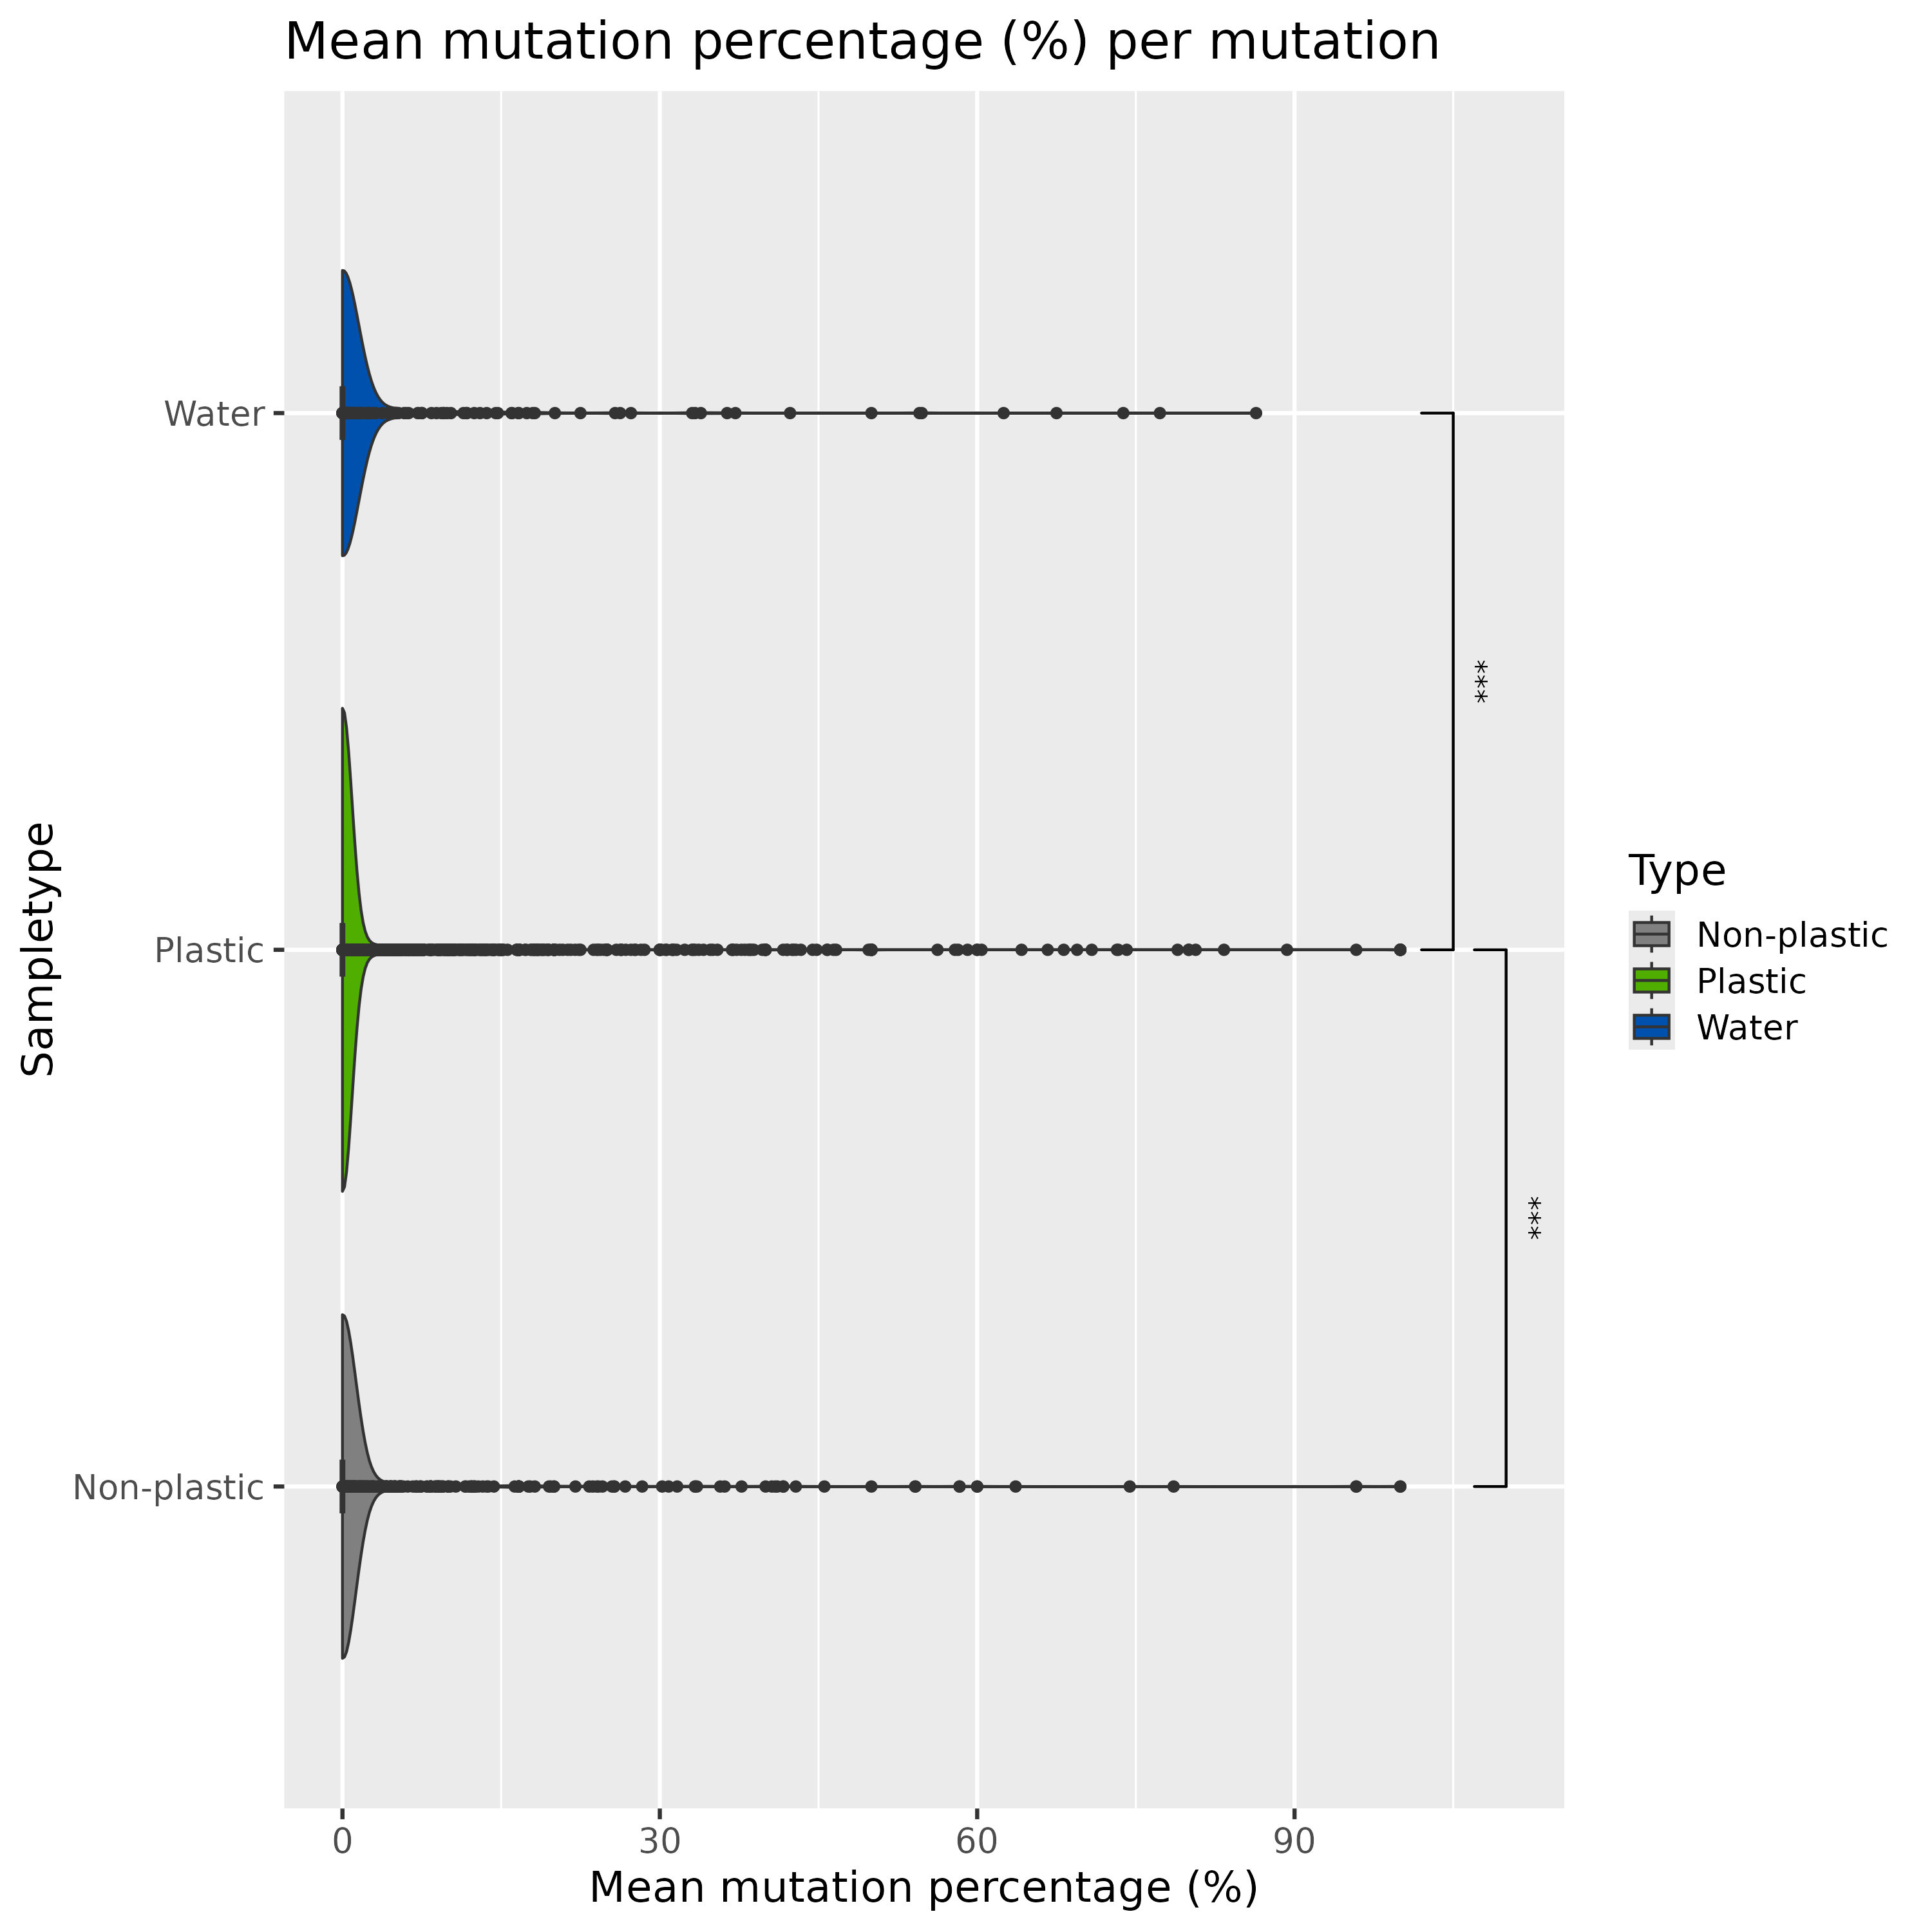
\includegraphics[width = 0.7\textwidth]{figure/mean_genes_sampletype.png}
    \caption{Mean mutation percentage (\%) per sample, grouped by sampletype. *** = p < 0.001}
    \label{mean_genes_sampletype}
\end{figure}

Figure \ref{mean_genes_substrate} show the mean mutation percentage per mutation grouped by substrate type. The figure shows that there are differences between the different substrates, and this is supported by figure \ref{wilcox_genes_substrate} which show the p-values from a Wilcoxon test between them, and that there are significant differences between many of them.
% Since figure \ref{mean_genes_substrate} uses a log-scale for visibility, the normal interpretation of the box-plot cannot be done since many points are erroneously removed, and therefore is only for visualizing the mutation rate.
The substrates which have the highest mean mutation percentage are PFP, PE, Ecovio, and BI-OPL from the plastic group as well as soil and wood from the non-plastic sampletypes. Freshwater had a significant increase to most other substrates.

% FROM samples substrates: 
% In figure \ref{mean_samples_substrate} the samples are instead grouped by substrate type, which show that there are differences for different plastics, as well as other substrates. Figure \ref{wilcox_samples_substrate} show the statistical significance of the comparison, when a wilcoxon test was done for the Substrate versus the Reference, as well as if there is an increase of the pseudo-mean compared to the reference. Note that all comparisons were done, but only the significant ones (p < 0.05) are shown. It is shown that there are some plastics that has a significant higher mean mutation percentage than most other substrates. These include PFP, LDPE, Ecovio and BI-OPL. The last two plastics are biodegradable plastics. The plastic substrates that has a significant higher mean mutation percentage than seawater or wastewater include PVC and PF in addition to the other plastics mentioned before. There are also some plastics which have significantly different lower mean mutation percentage than almost all other substrates, the most notable of which is high-density polyethylene (HDPE), poly(3-hydroxybutyrate-co-3-hydroxyvalerate) (PHBV) and polyhydroxyalkanoate (PHA), of which the latter two are biodegradable polymers while the first one is not. Almost all substrates has a significantly different lower mean mutation percentage than the freshwater samples, the exception of which is leaf, rock, Ecovio, BI-OPL, and PFP where there is no significant difference. The soil samples also has a significant higher mean mutation percentage compared to many other substrates.

\begin{figure}[h!]
    \centering
    \subfloat[\label{mean_genes_substrate}]{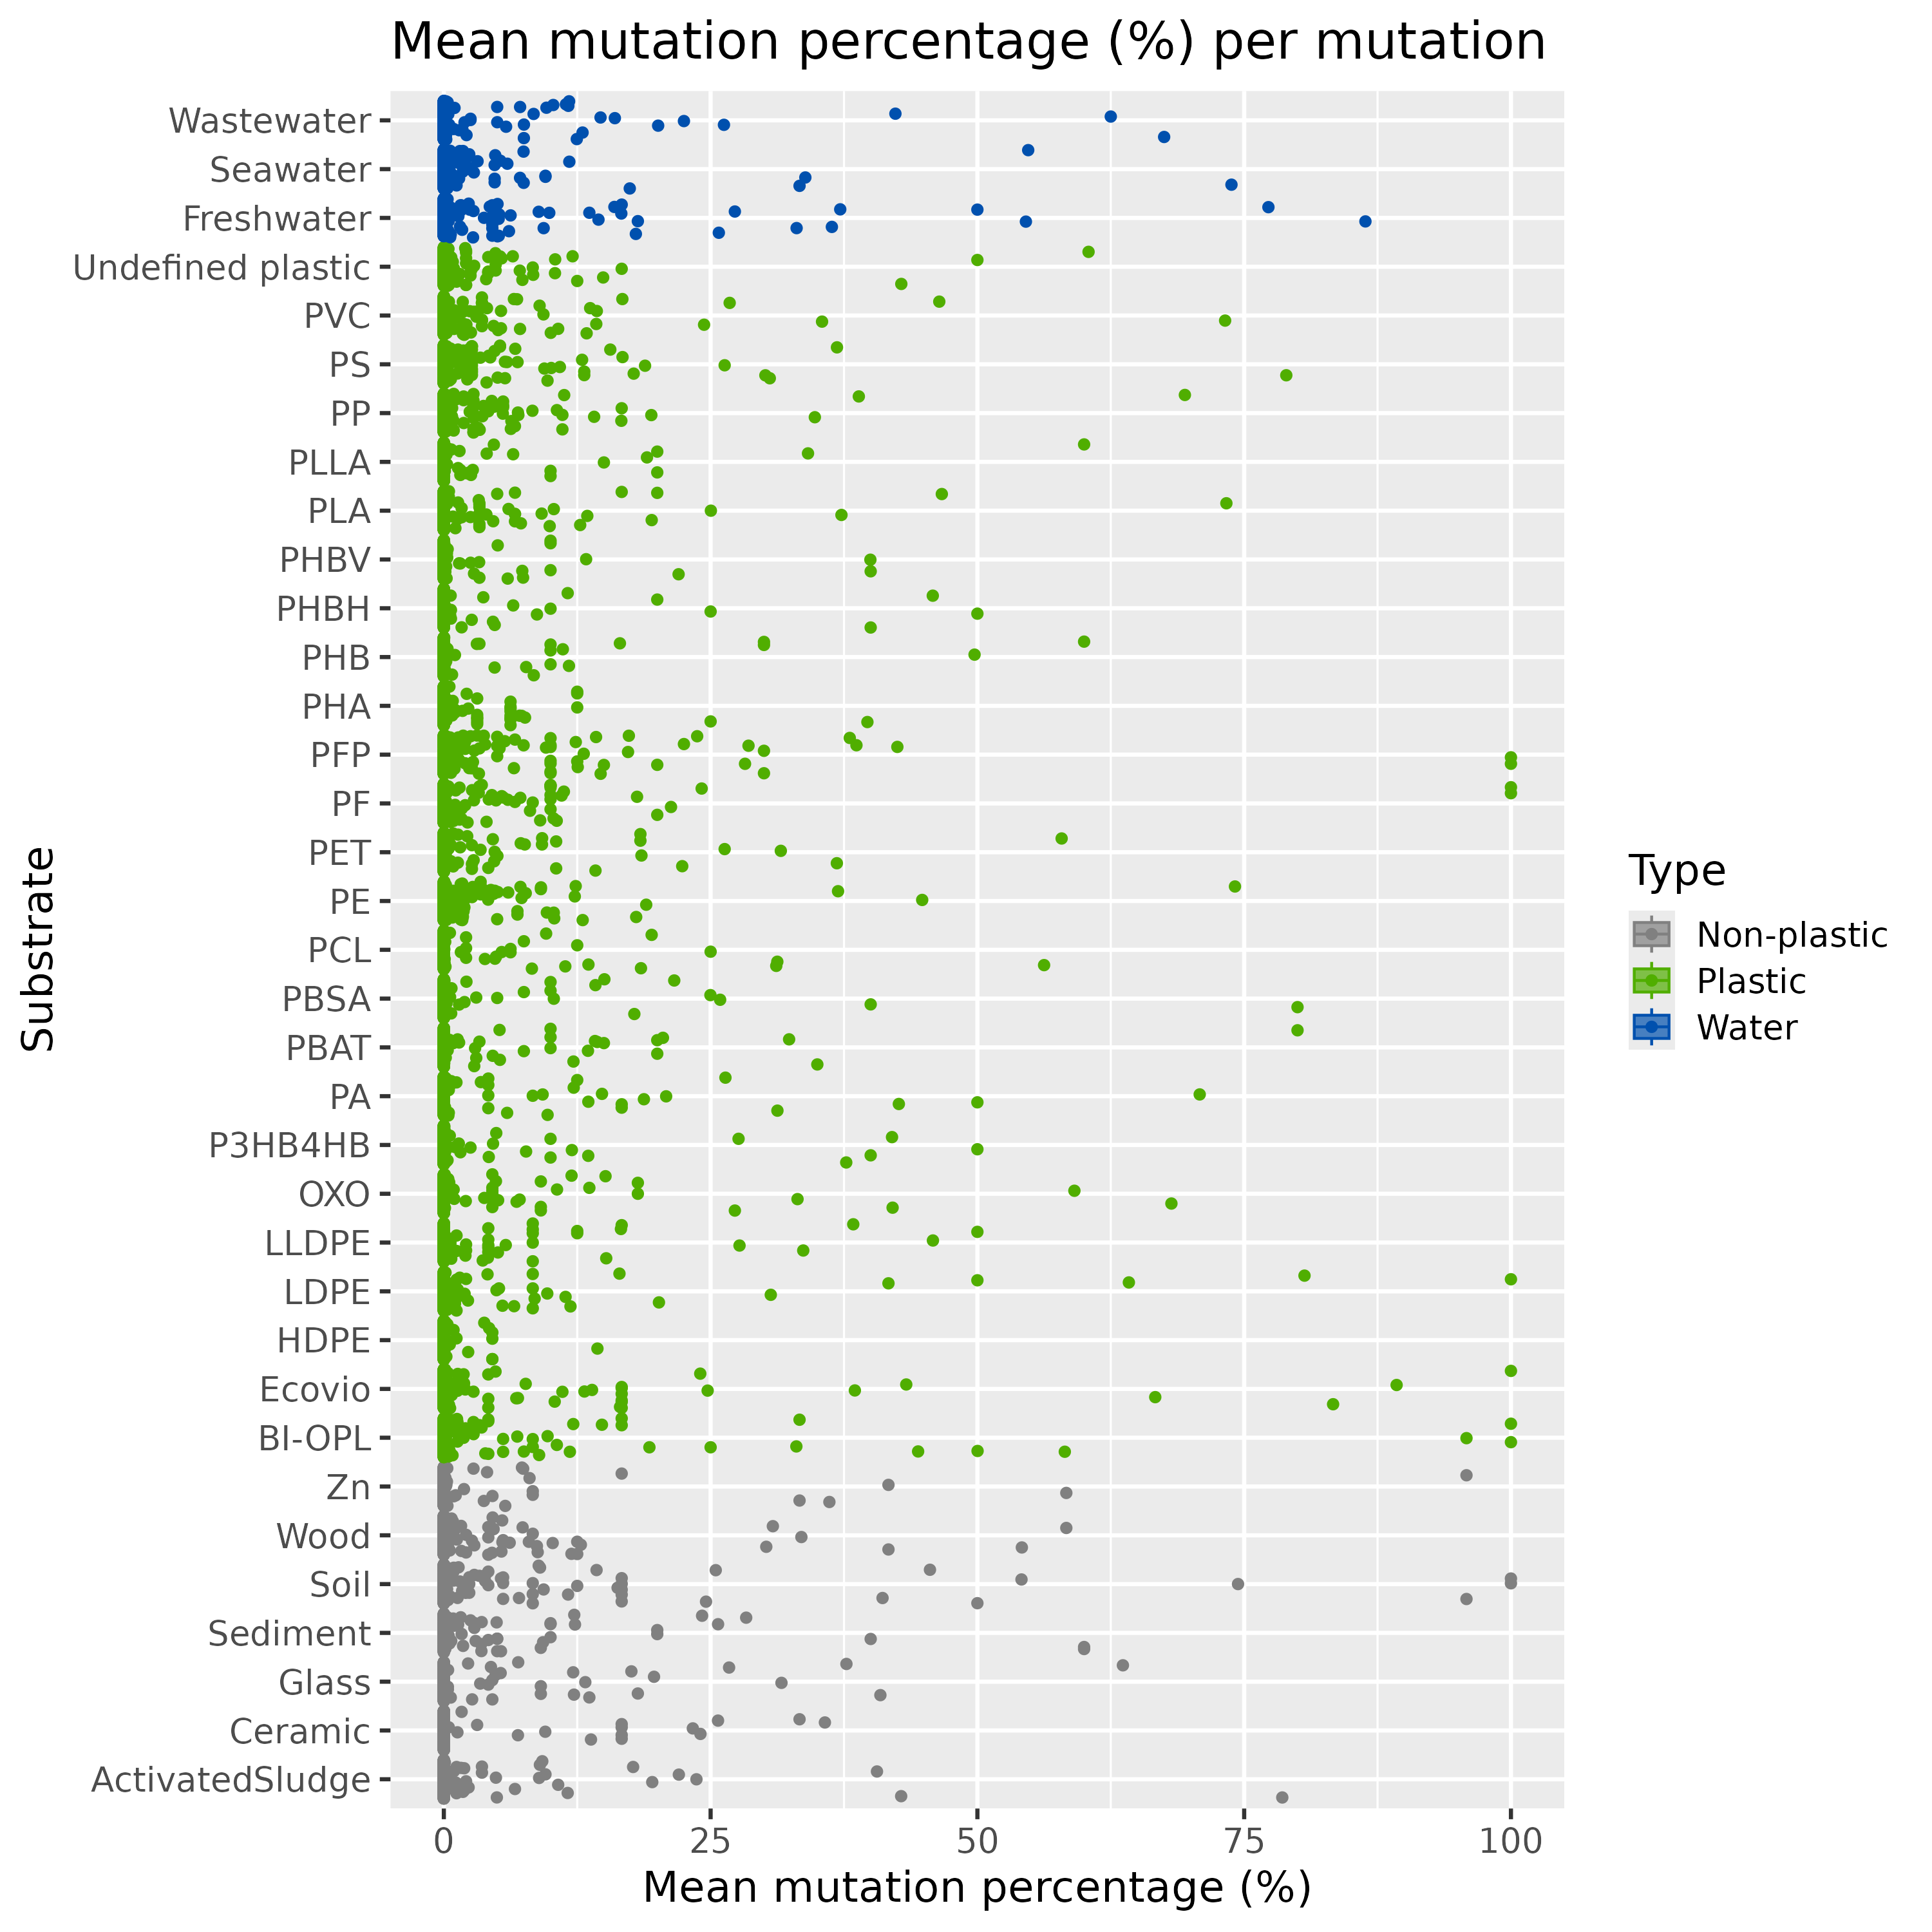
\includegraphics[width=0.5\textwidth]{figure/mean_genes_substrate.png}} 
    \subfloat[\label{wilcox_genes_substrate}]{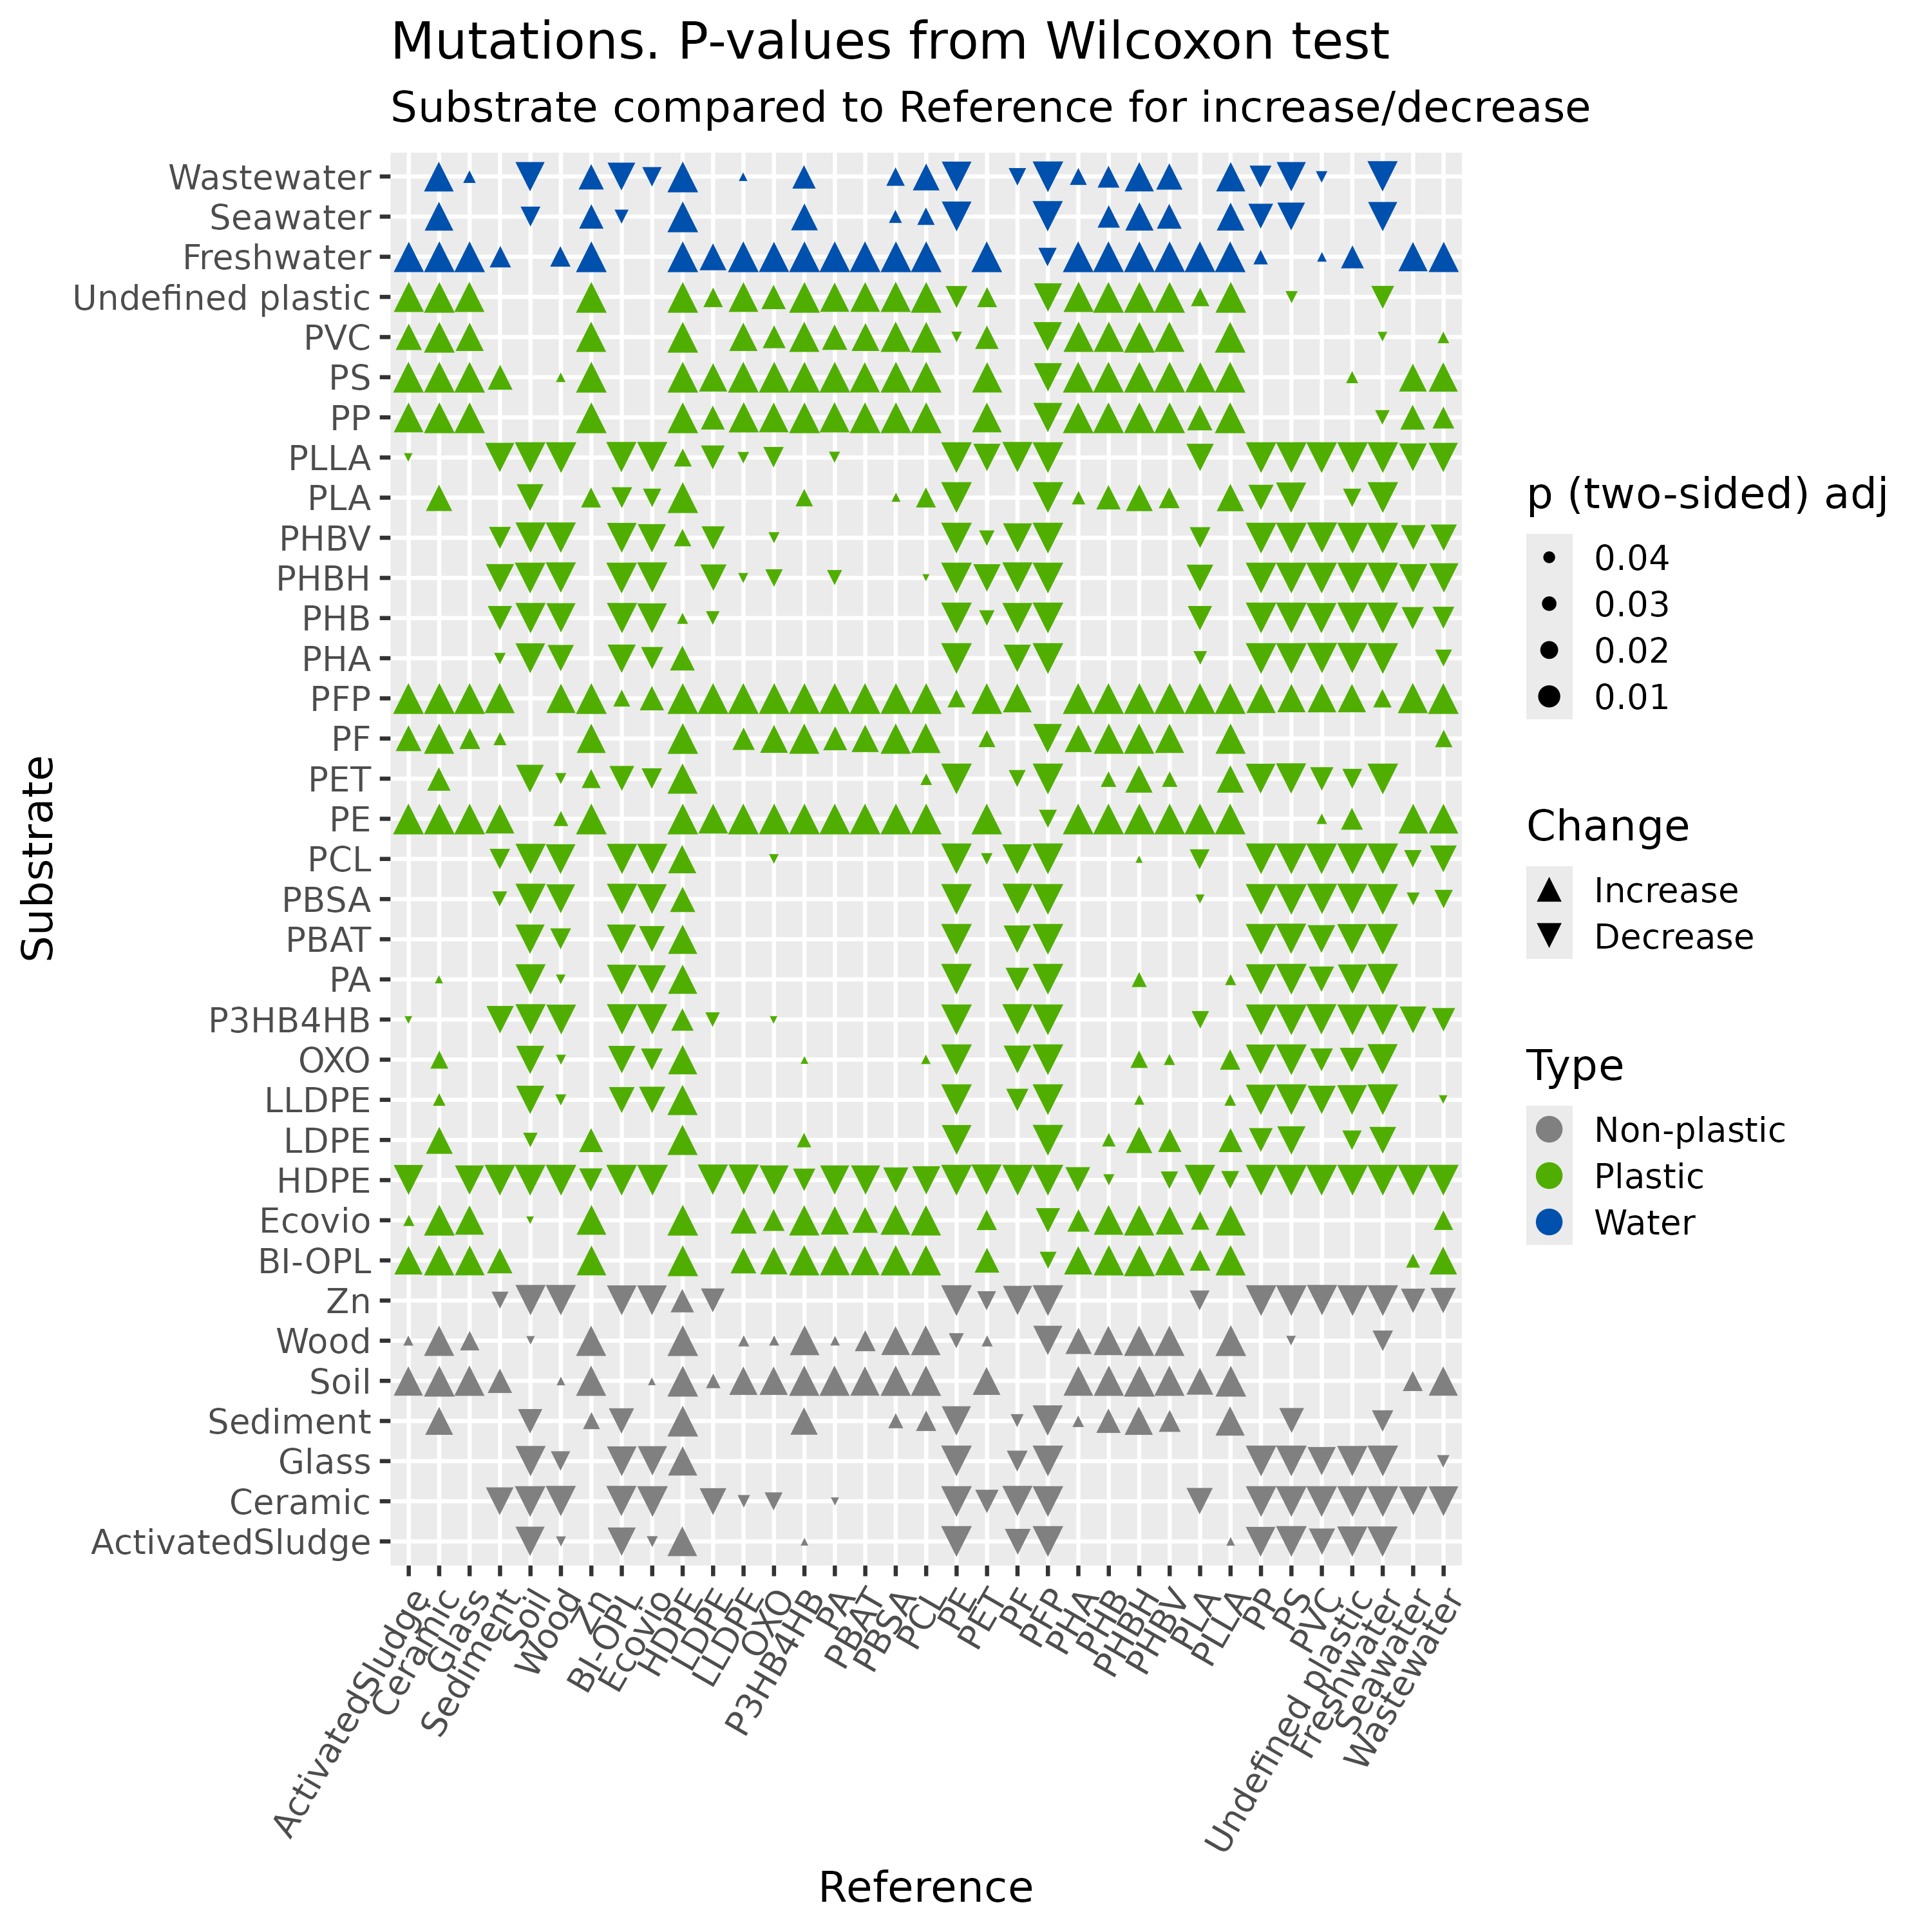
\includegraphics[width=0.5\textwidth]{figure/wilcox_genes_substrates.png}}
    \caption{(a) Mean mutation percentage per mutation, grouped by substrate type. (b) p-values from Wilcoxon test of mean mutation percentage for Substrate versus Reference}
    \label{both_mean_genes_substrate}
\end{figure}

Figure \ref{pointplot_mutations} show the mean mutation percentage for point mutations with a mean mutation percentage higher than 25 percent in any substrate. 
The figure shows that there are certain mutations which occur in most substrates and some that only ooccur in some substrates. The ones which occur in almost all samples are Q1073R in rpoB which confer resistance to rifampicin, G1245B in gyrB which confer resistance to aminocoumarin, and D244Y in rpoC which confer resistance to vancomycin. \todo{Mention Ecovio, BI-OPL, PFP, Freshwater, Soil with many point mutations of high mean mutation percentage?}

\begin{figure}[!h]
    \centering
    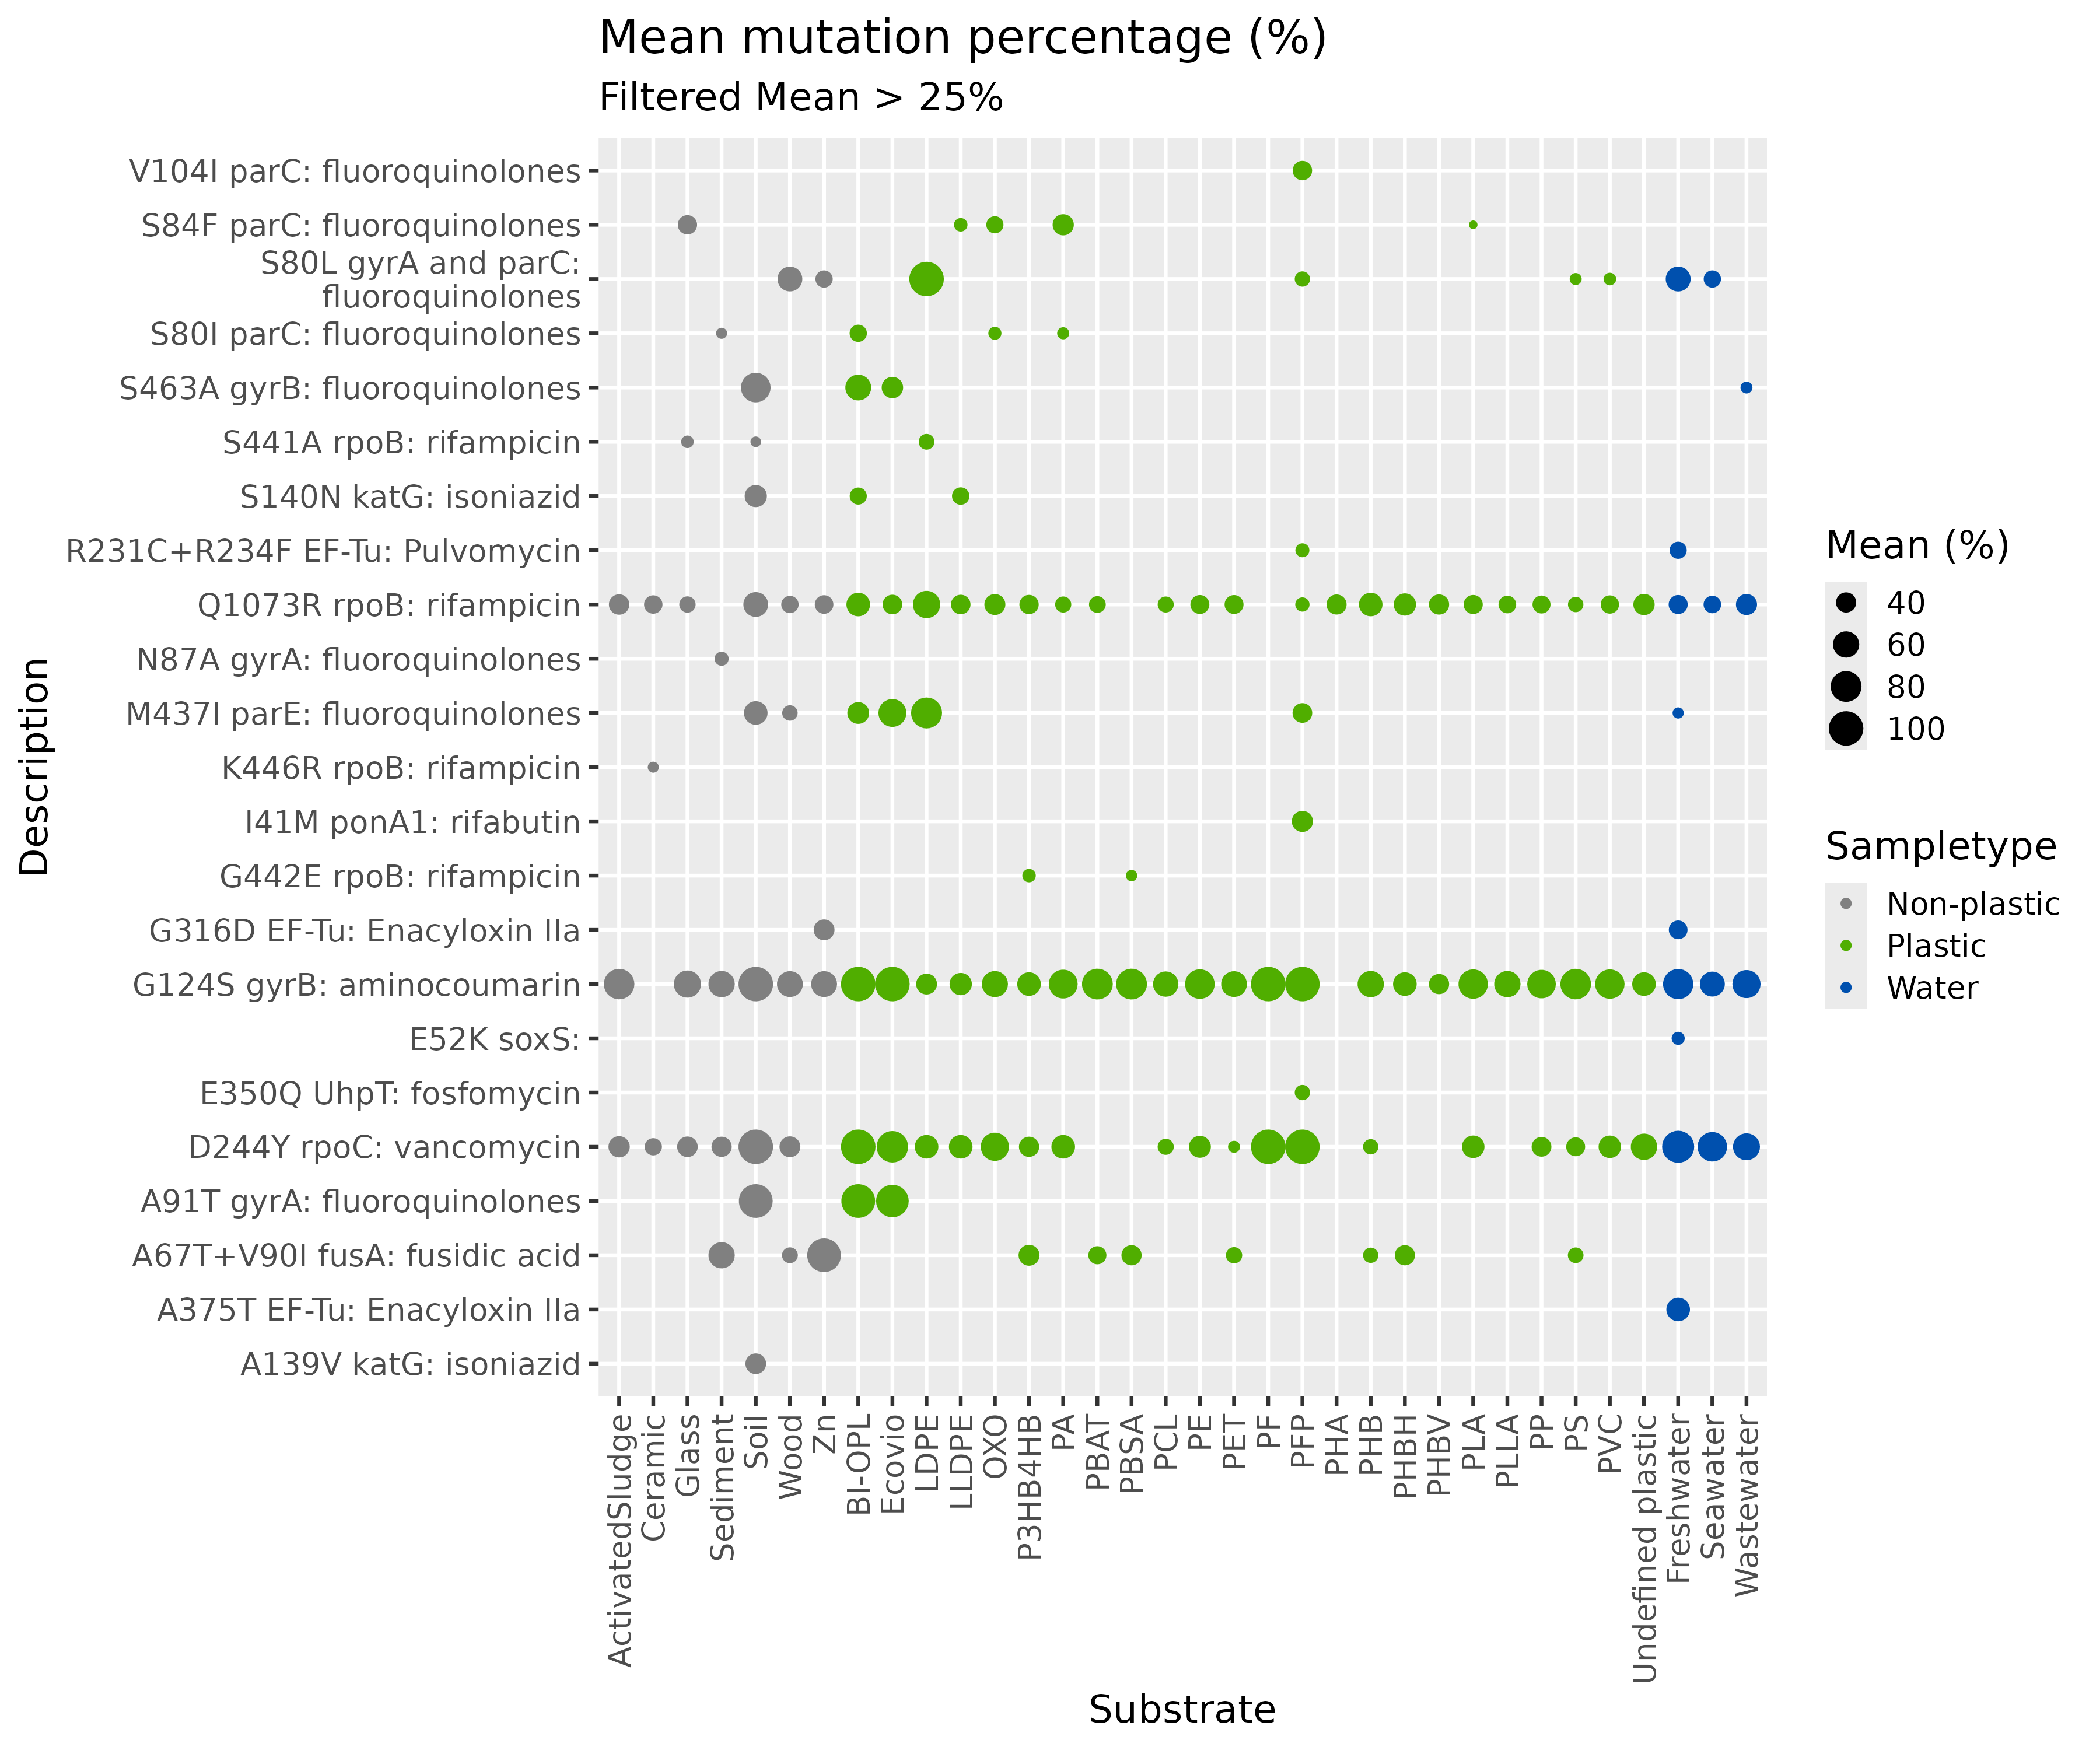
\includegraphics[width = \textwidth]{figure/relative_mean_points_25.png}
    \caption{Filtered mean mutation percentage per mutation. TODO: include this or skip?}
    \label{pointplot_mutations}
\end{figure}


\section{Predicting substrate identifiers} 
\todo{Rename from Random Forest to something else}
%TODO Rename to something else, "Predicting sample  
% Removed:
% D87H:Pseudomonas aeruginosa gyrA: fluoroquinolones
% D87H:Burkholderia dolosa gyrA: fluoroquinolones
%
% Renamed: There is one AMR Gene Family which has a very long name:
% "ATP-binding cassette (ABC) antibiotic efflux pump;General Bacterial Porin with reduced permeability to beta-lactams;major facilitator superfamily (MFS) antibiotic efflux pump;resistance-nodulation-cell division (RND) antibiotic efflux pump"
In the following figures only the ten most significant AMR Gene Families or mutations are shown. However, there are in all cases several more which are not shown. 
Figures showing all the 50 most significant variables can be found in Appendix \ref{appendix:code}.
\todo{Do this? Not sure if \emph{all} of them can be shown, but at least 50 is possible in a really long plot}

\subsection{AMR Gene Family}
In the database CARD, each mutation is associated with an AMR Gene Family, which is a classification tag such as "rifampicin resistant rpoC" or "fluoroquinolone resistant parC". The AMR Gene Family is used in this analysis since it enables us to group the mutations by gene and conferred antibiotic resistance.
%in order to identify the function of the mutations present in the samples.

%\subsubsection{Sampletypes}
Based on the mean decrease in Gini impurity, certain AMR Gene families were significantly (p < 0.001) assigned to the non-plastic sampletype, as shown in figure \ref{amr_sampletype}. These included fluoroquinolone resistant parC and gyrA as well as daptomycin-resistant beta-subunit of RNA polymerase (rpoB). 
%Figure \ref{amr_sampletype_bar} show the mean decrease in Gini impurity for five different AMR Gene Families, which was found to be significant.
%{true or not? true since kruskal-wallace test found X taxa singificant} when the samples are grouped by sampletype.
%Three of the families may be used to identify the non-plastic samples, which include fluoroquinolone resistant parC and gyrA as well as daptomycin-resistant beta-subunit of RNA polymerase (rpoB). 
The two significant AMR Gene Families for the water samples were vancomycin-resistant beta prime subunit of RNA polymerase (rpoC) and rifampicin-reistant rpoC. 
However, note the negative sign of these which indicate that these AMR Gene Families are more important to determine that a sample is in the reference group (the other groups) than in the water group. 
%\{It is significant, shows that a samples is NOT in the water group. As mentioned above. Can only say that a sample is from the non-plastic group, or NOT in the water group, not the abundance of it.}

\begin{figure}[h]
    \centering
    \subfloat[\label{amr_sampletype_bar}]{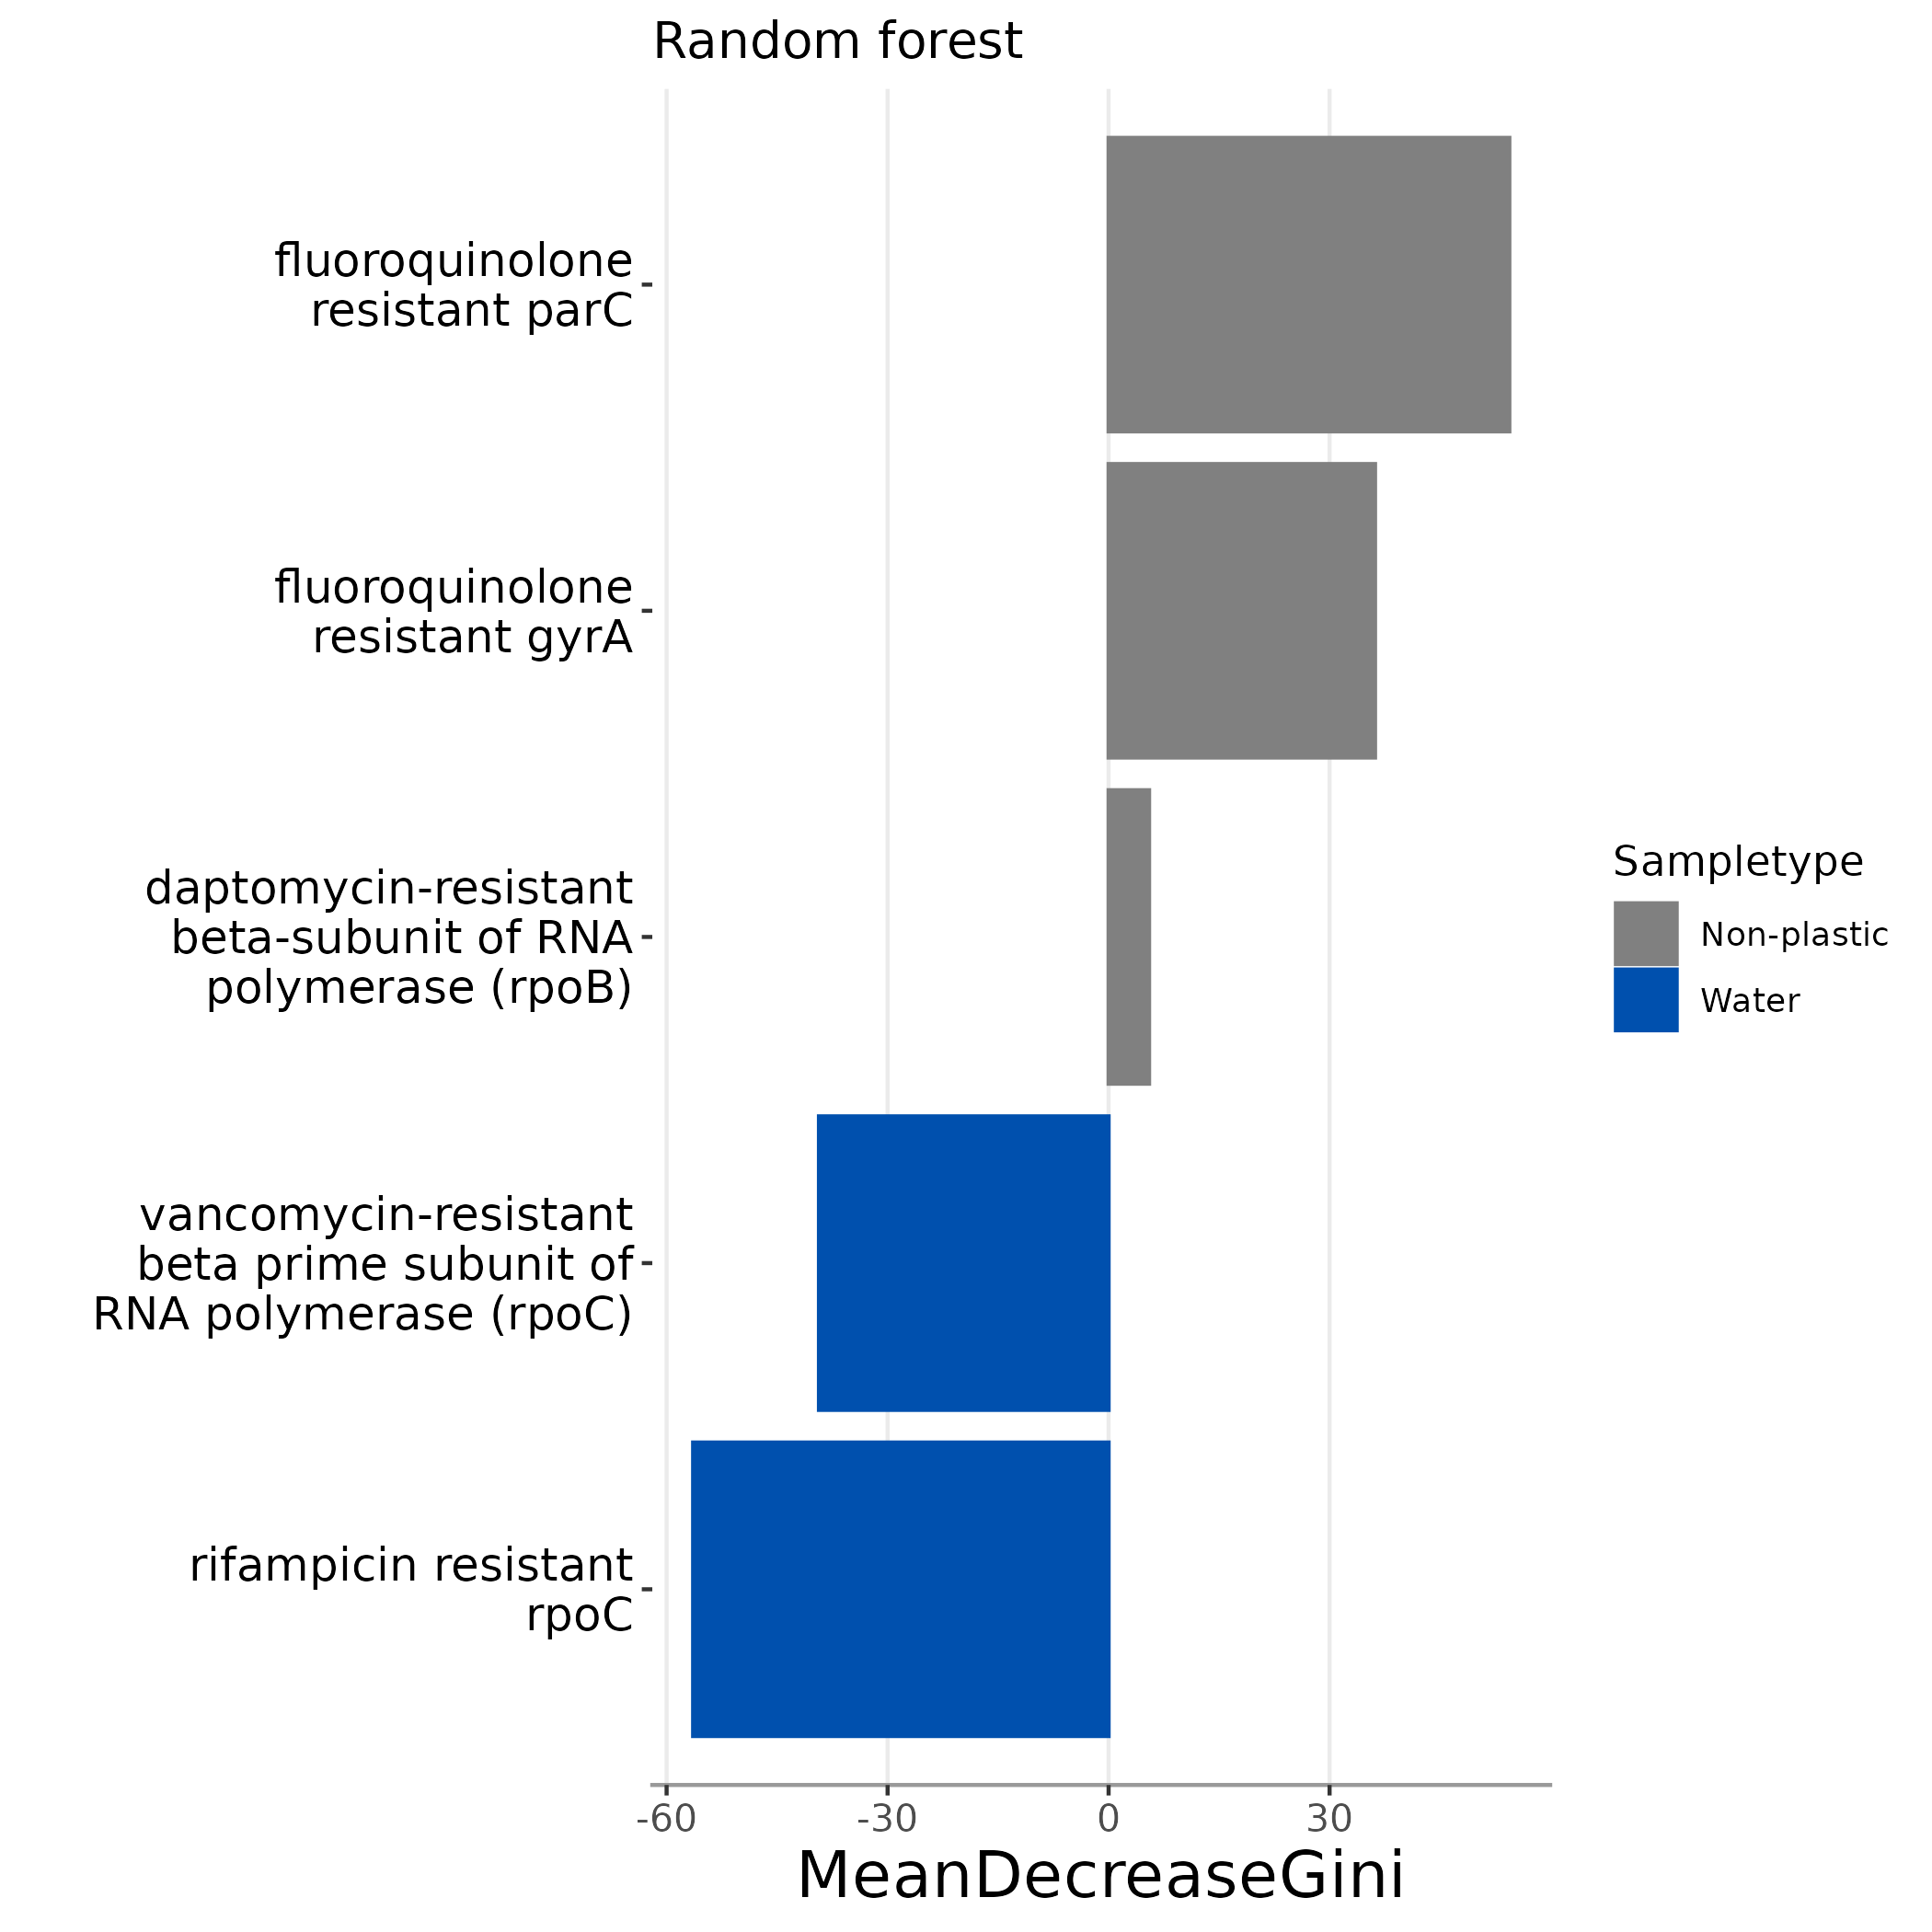
\includegraphics[width=0.5\textwidth]{figure/relative_forest_sampletype_amr_bar.png}}
    \subfloat[\label{amr_sampletype_abund}]{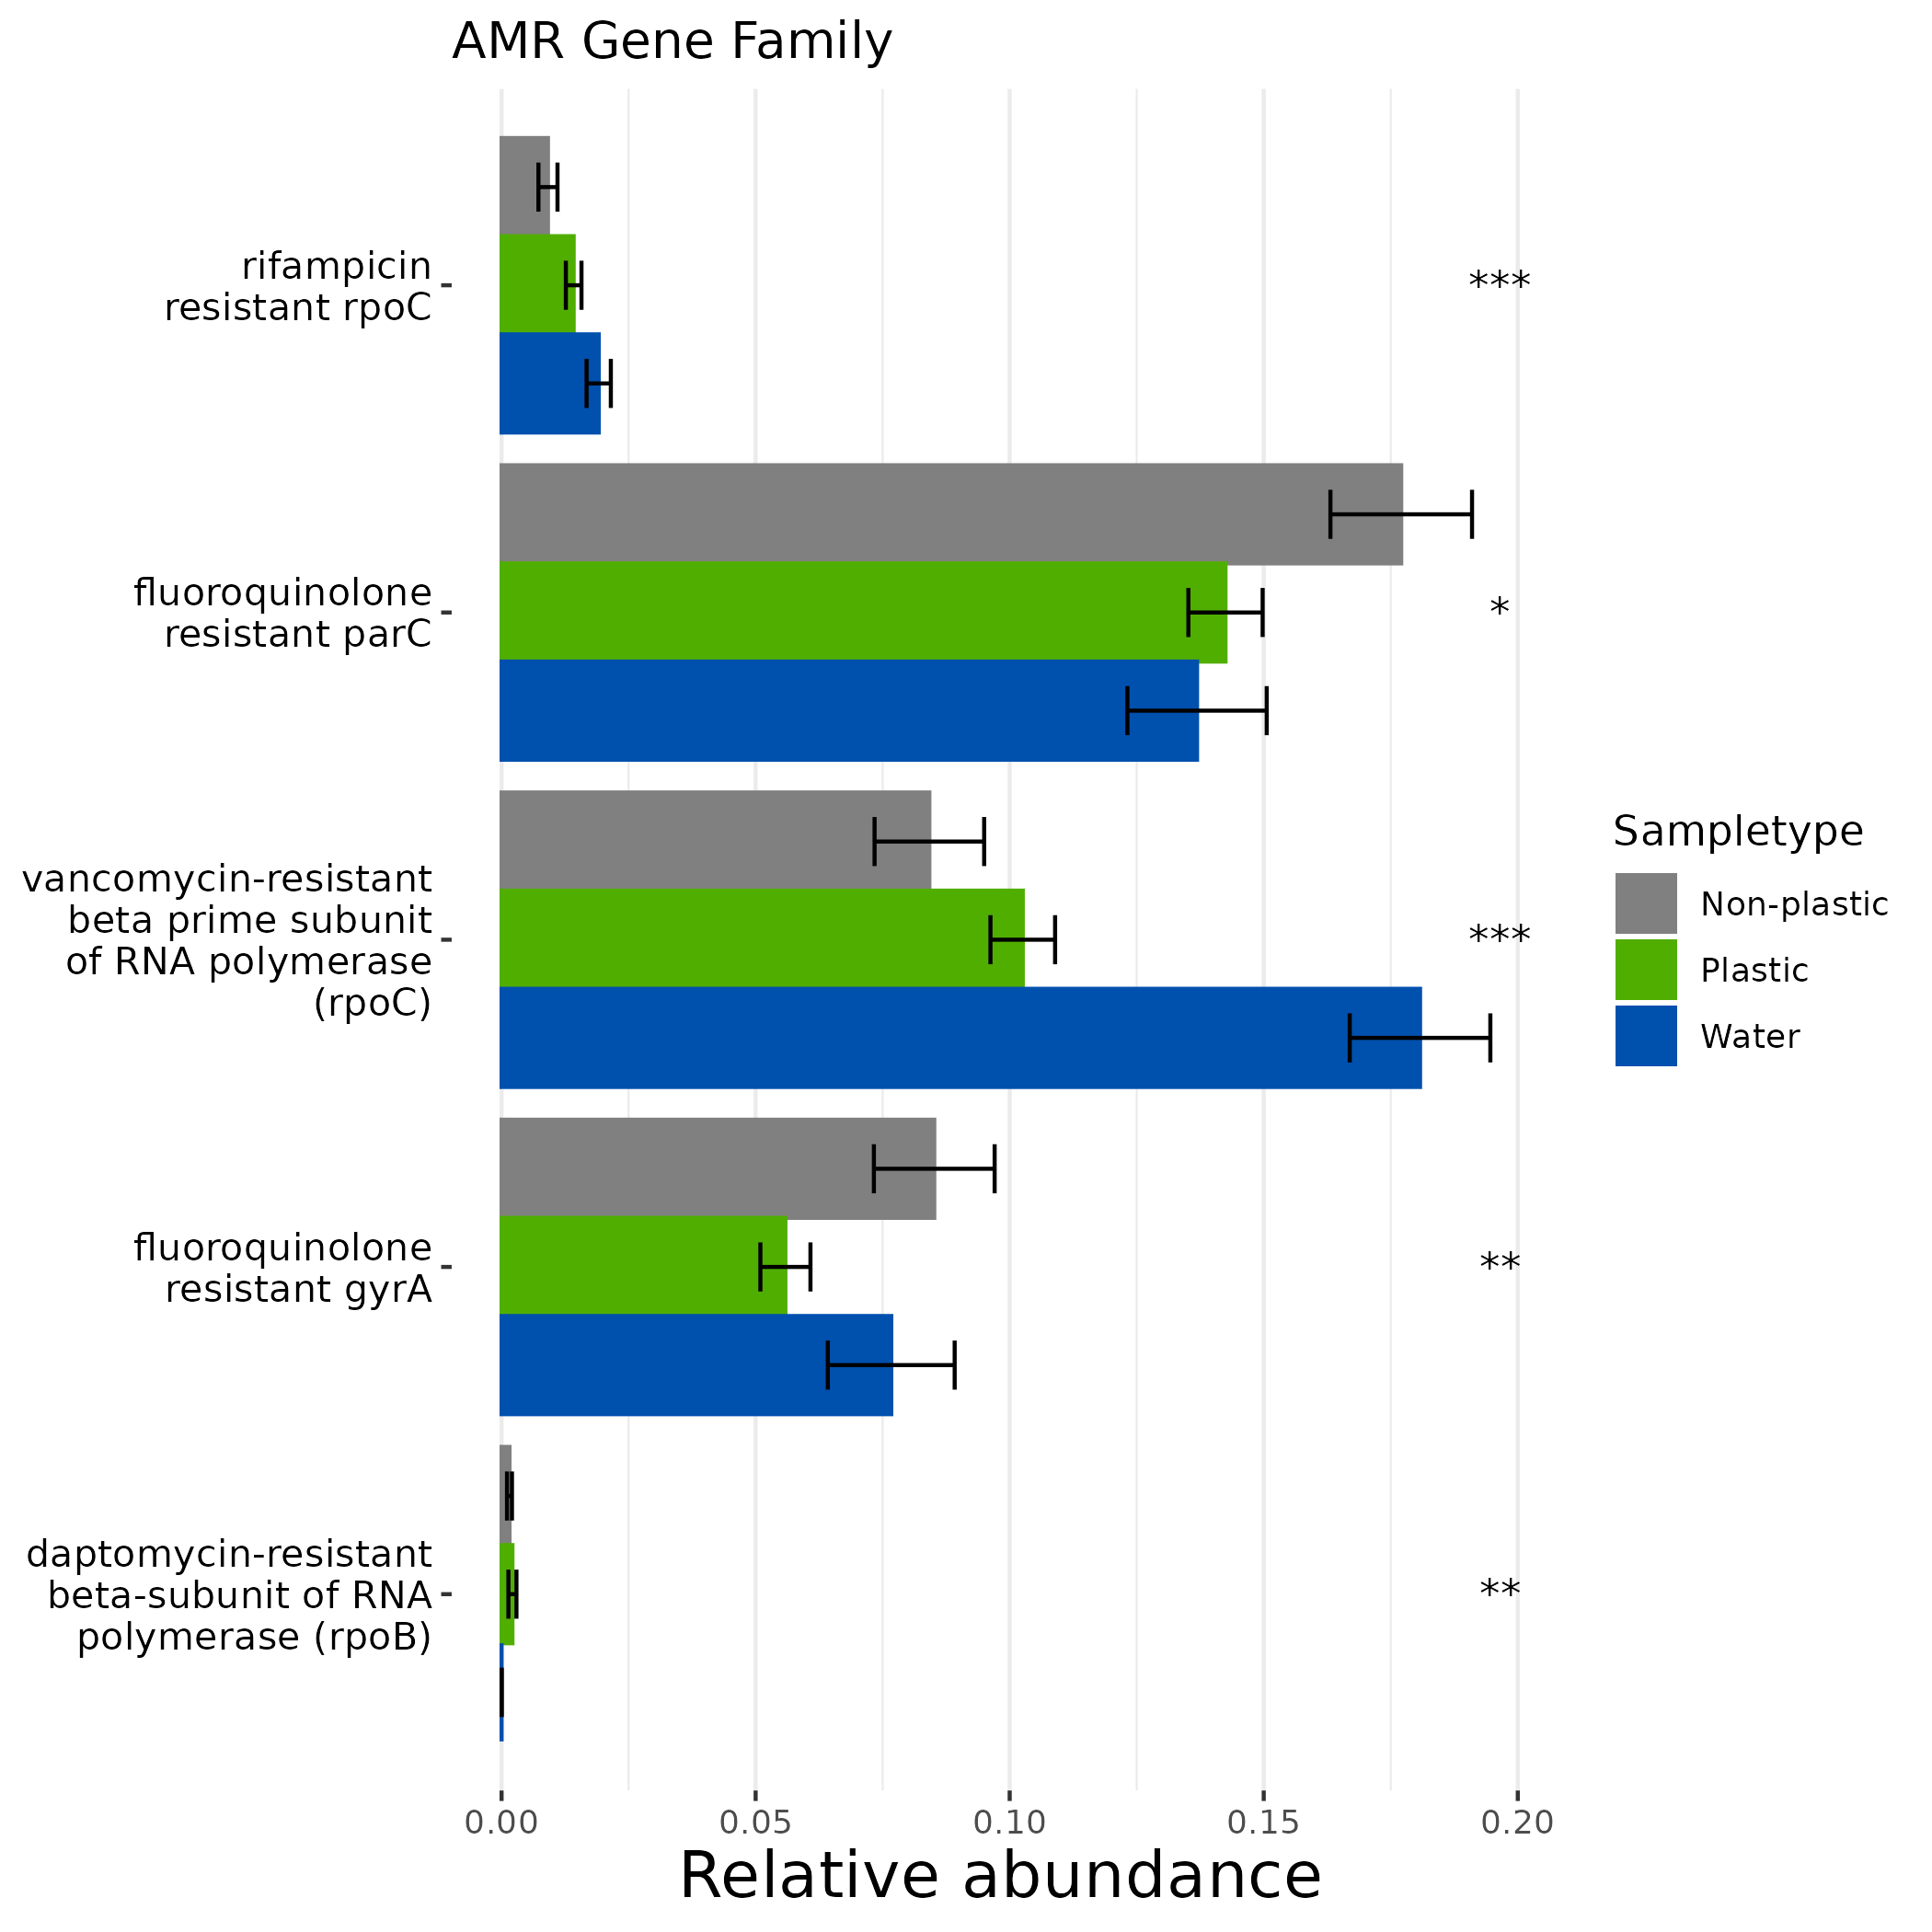
\includegraphics[width=0.5\textwidth]{figure/relative_forest_sampletype_amr_abund.png}}
    \caption{(a) Significantly assigned AMR Gene Families and Mean Decrease Gini Importance when grouped by sampletype. (b) Relative Abundances of the different AMR Gene Families in the sampletype}
    \label{amr_sampletype}
\end{figure}

If instead the samples are grouped by substrate type, as shown in figure \ref{amr_substrate_bar}, there are a lot more AMR Gene Families which distinguishes the samples in one group from another.
The most prevalent substrate in this figure is the activated sludge, which has four different AMR Gene Families that distinguishes it.
The one labelled Multiple Resistant Variants has been renamed from "ATP-binding cassette (ABC) antibiotic efflux pump; General Bacterial Porin with reduced permeability to beta-lactams; major facilitator superfamily (MFS) antibiotic efflux pump; resistance-nodulation-cell division (RND) antibiotic efflux pump". 
%\{comment or just observation?}
All Mean Decrease Gini impurity values are positive for this grouping, there are no significant AMR Gene Families which indicates that a sample is not from a specific substrate as was the case with the water sampletype. 

\begin{figure}[!h]
    \centering
    \subfloat[\label{amr_substrate_bar}]{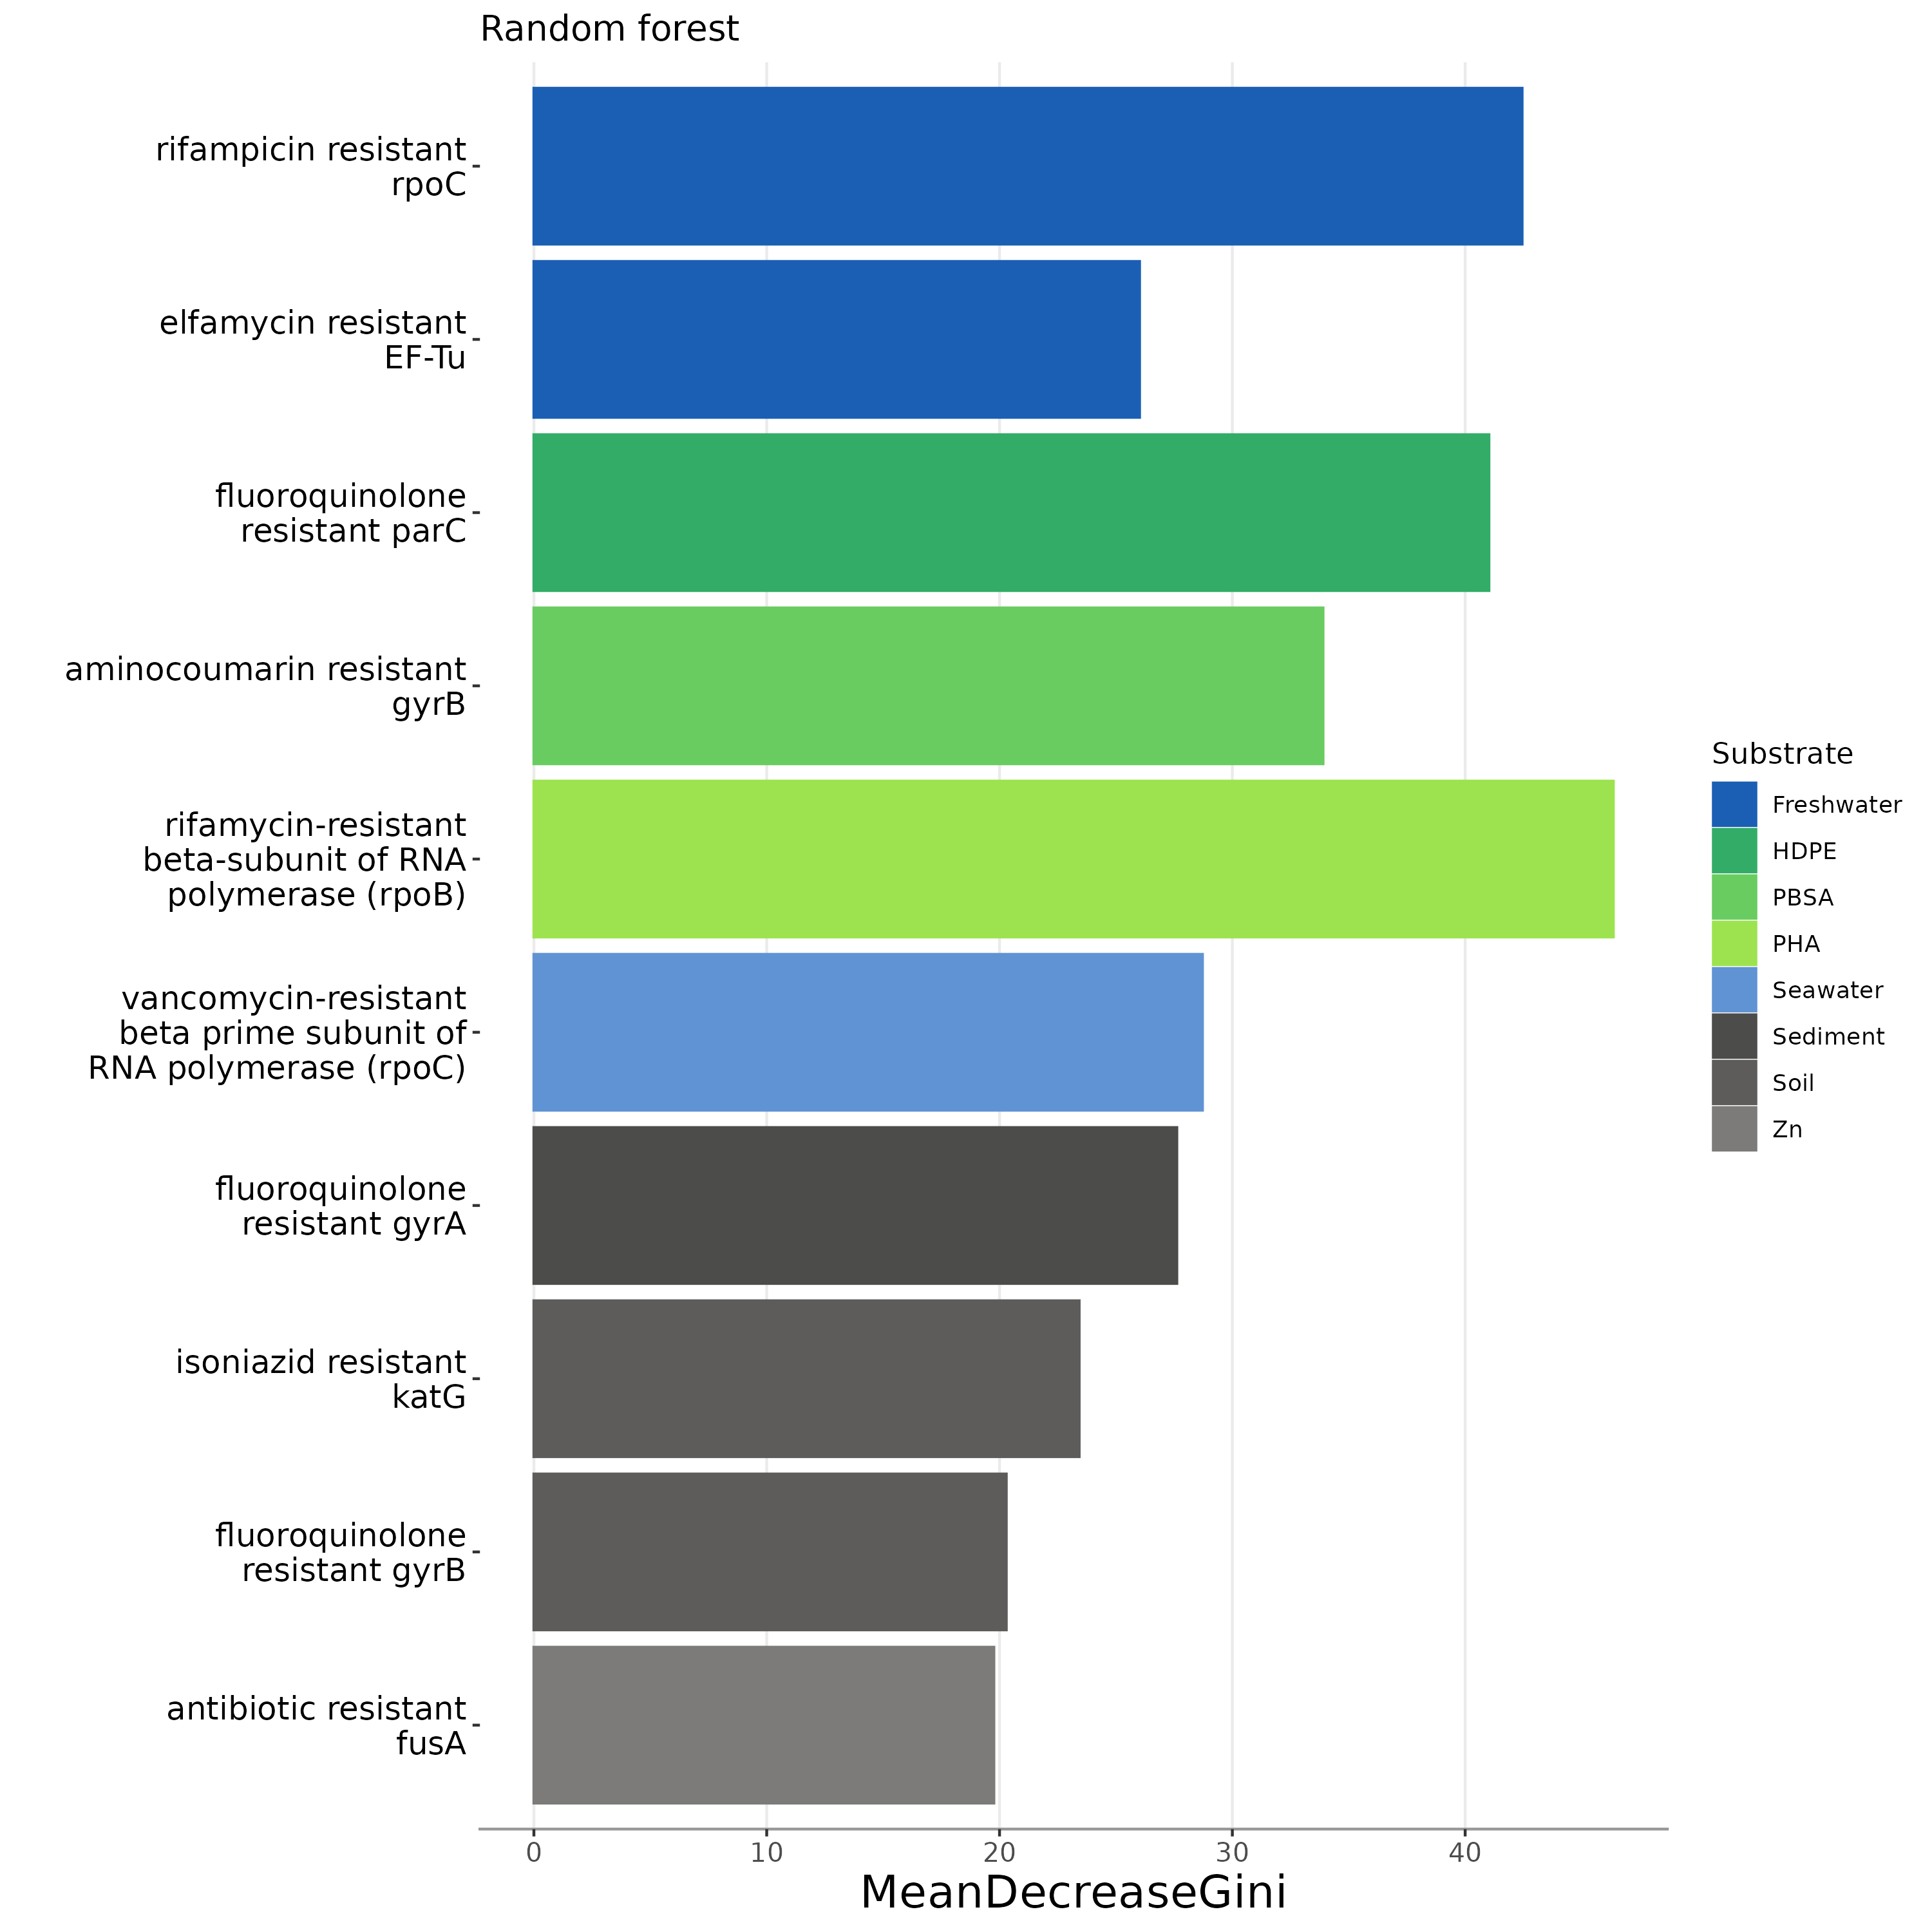
\includegraphics[width=0.5\textwidth]{figure/relative_forest_substrate_amr_bar.png}}
    \subfloat[\label{amr_substrate_abund}]{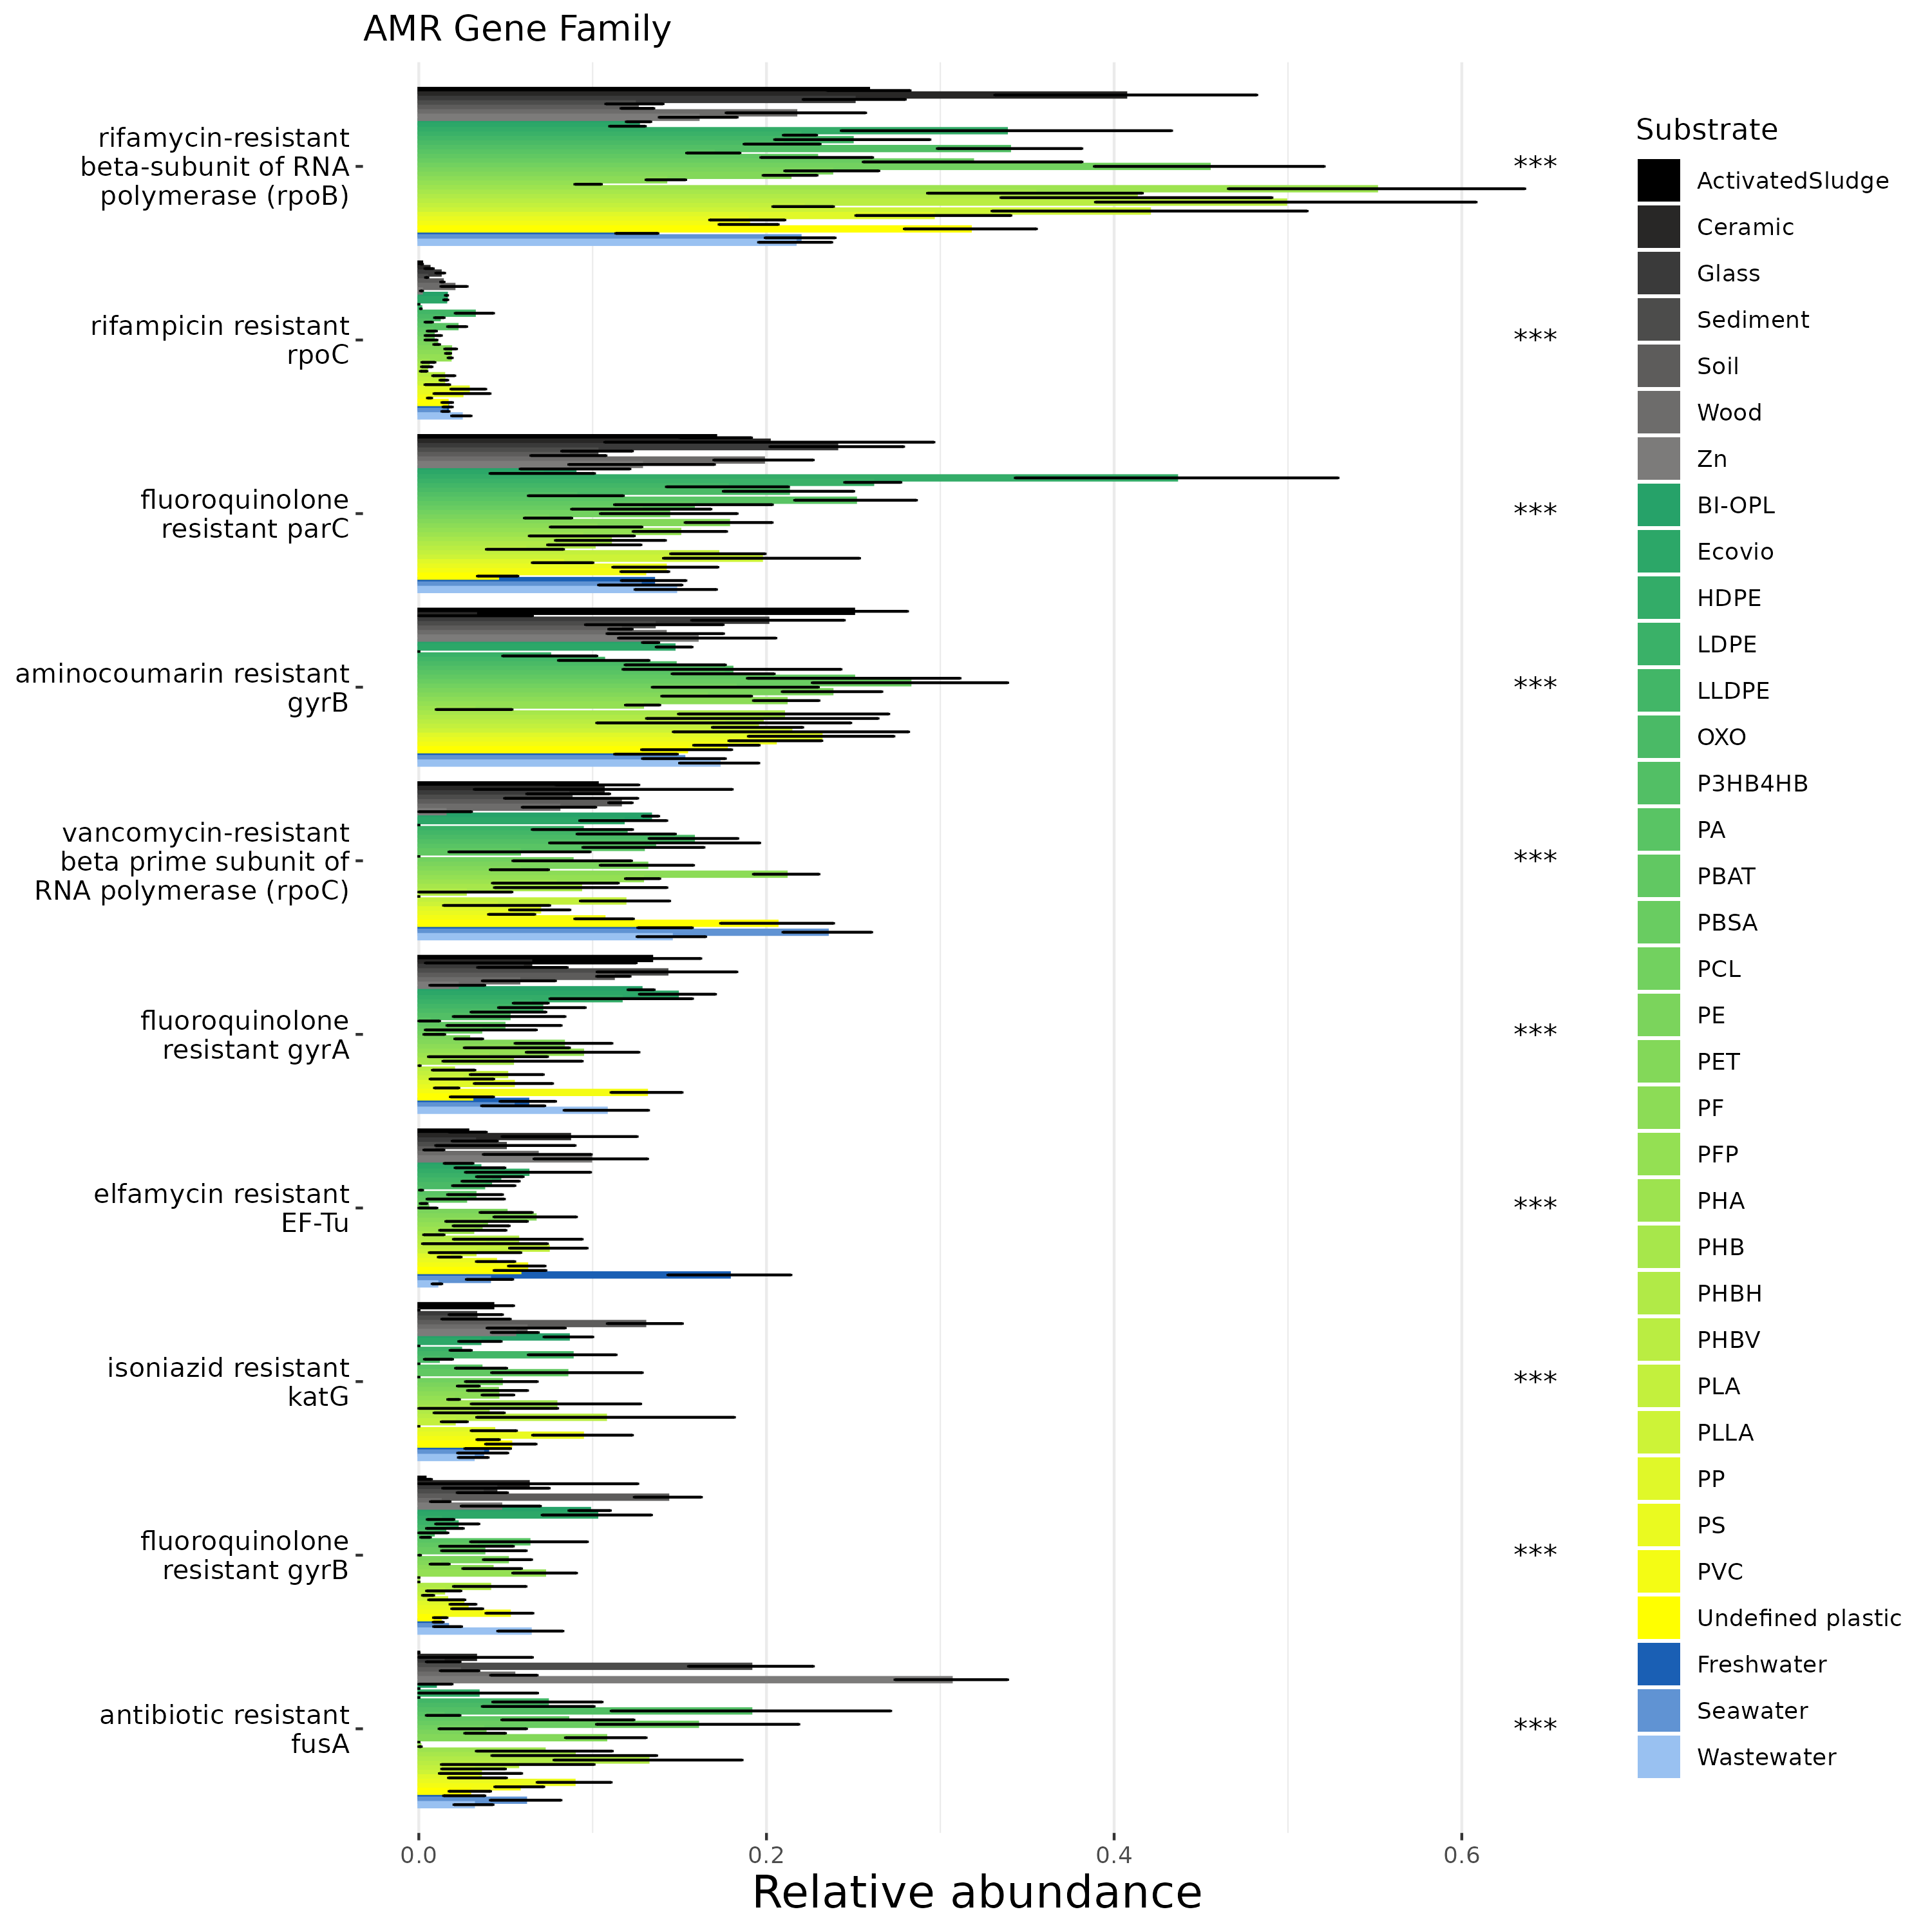
\includegraphics[width=0.5\textwidth]{figure/relative_forest_substrate_amr_abund.png}}
    \caption{(a) Significantly assigned AMR Gene Families and Mean Decrease Gini Importance when grouped by substrate. (b) Relative Abundances of the different AMR Gene Families in the substrates}
    \label{amr_substrate}
\end{figure}

\subsection{Prediciting point mutations as substrate identifiers} \todo{Predicting identity using point mutation} \todo{Substrate prediction using point mutations} \todo{Prediciting substrate identifiers using point mutations}
The following figures use the individual point mutations, or combinations thereof, found in the samples as the grouping for which the random forest analysis was performed, instead of the AMR Gene Family. 
Only the non-plastic sampletype can be significantly assigned (p < 0.05) to any mutation in figure \ref{snps_sampletype}, which includes several mutations in rpoB which confer resistance to rifampicin, as well as several in gyrA and parC which confer resistance to fluoroquinolones. 
As for the assignment to the AMR Gene Families, the water sampletype cannot be assigned to any specific point mutations directly. However one can assign a greater importance to the reference group, which consists of the two other sampletypes, than the water group for two mutations which both occur in rpoC.

%Figure \ref{snp_sampletype_bar} show the result of the analysis using the three different sampletypes as grouping, and as above only the non-plastic group and the water group are present. 
%The significant mutations for the non-plastic group include several mutations in rpoB which confer resistance to rifampicin, as well as several in gyrA and parC which confer resistance to fluoroquinolones.
%There is one combination of four mutations in rpoB which confer resistance to rifampicin. 
%However, the abundance of these mutations is relatively low, as is shown in figure \ref{snp_sampletype_abund}.

\begin{figure}[h]
    \centering
    \subfloat[\label{snp_sampletype_bar}]{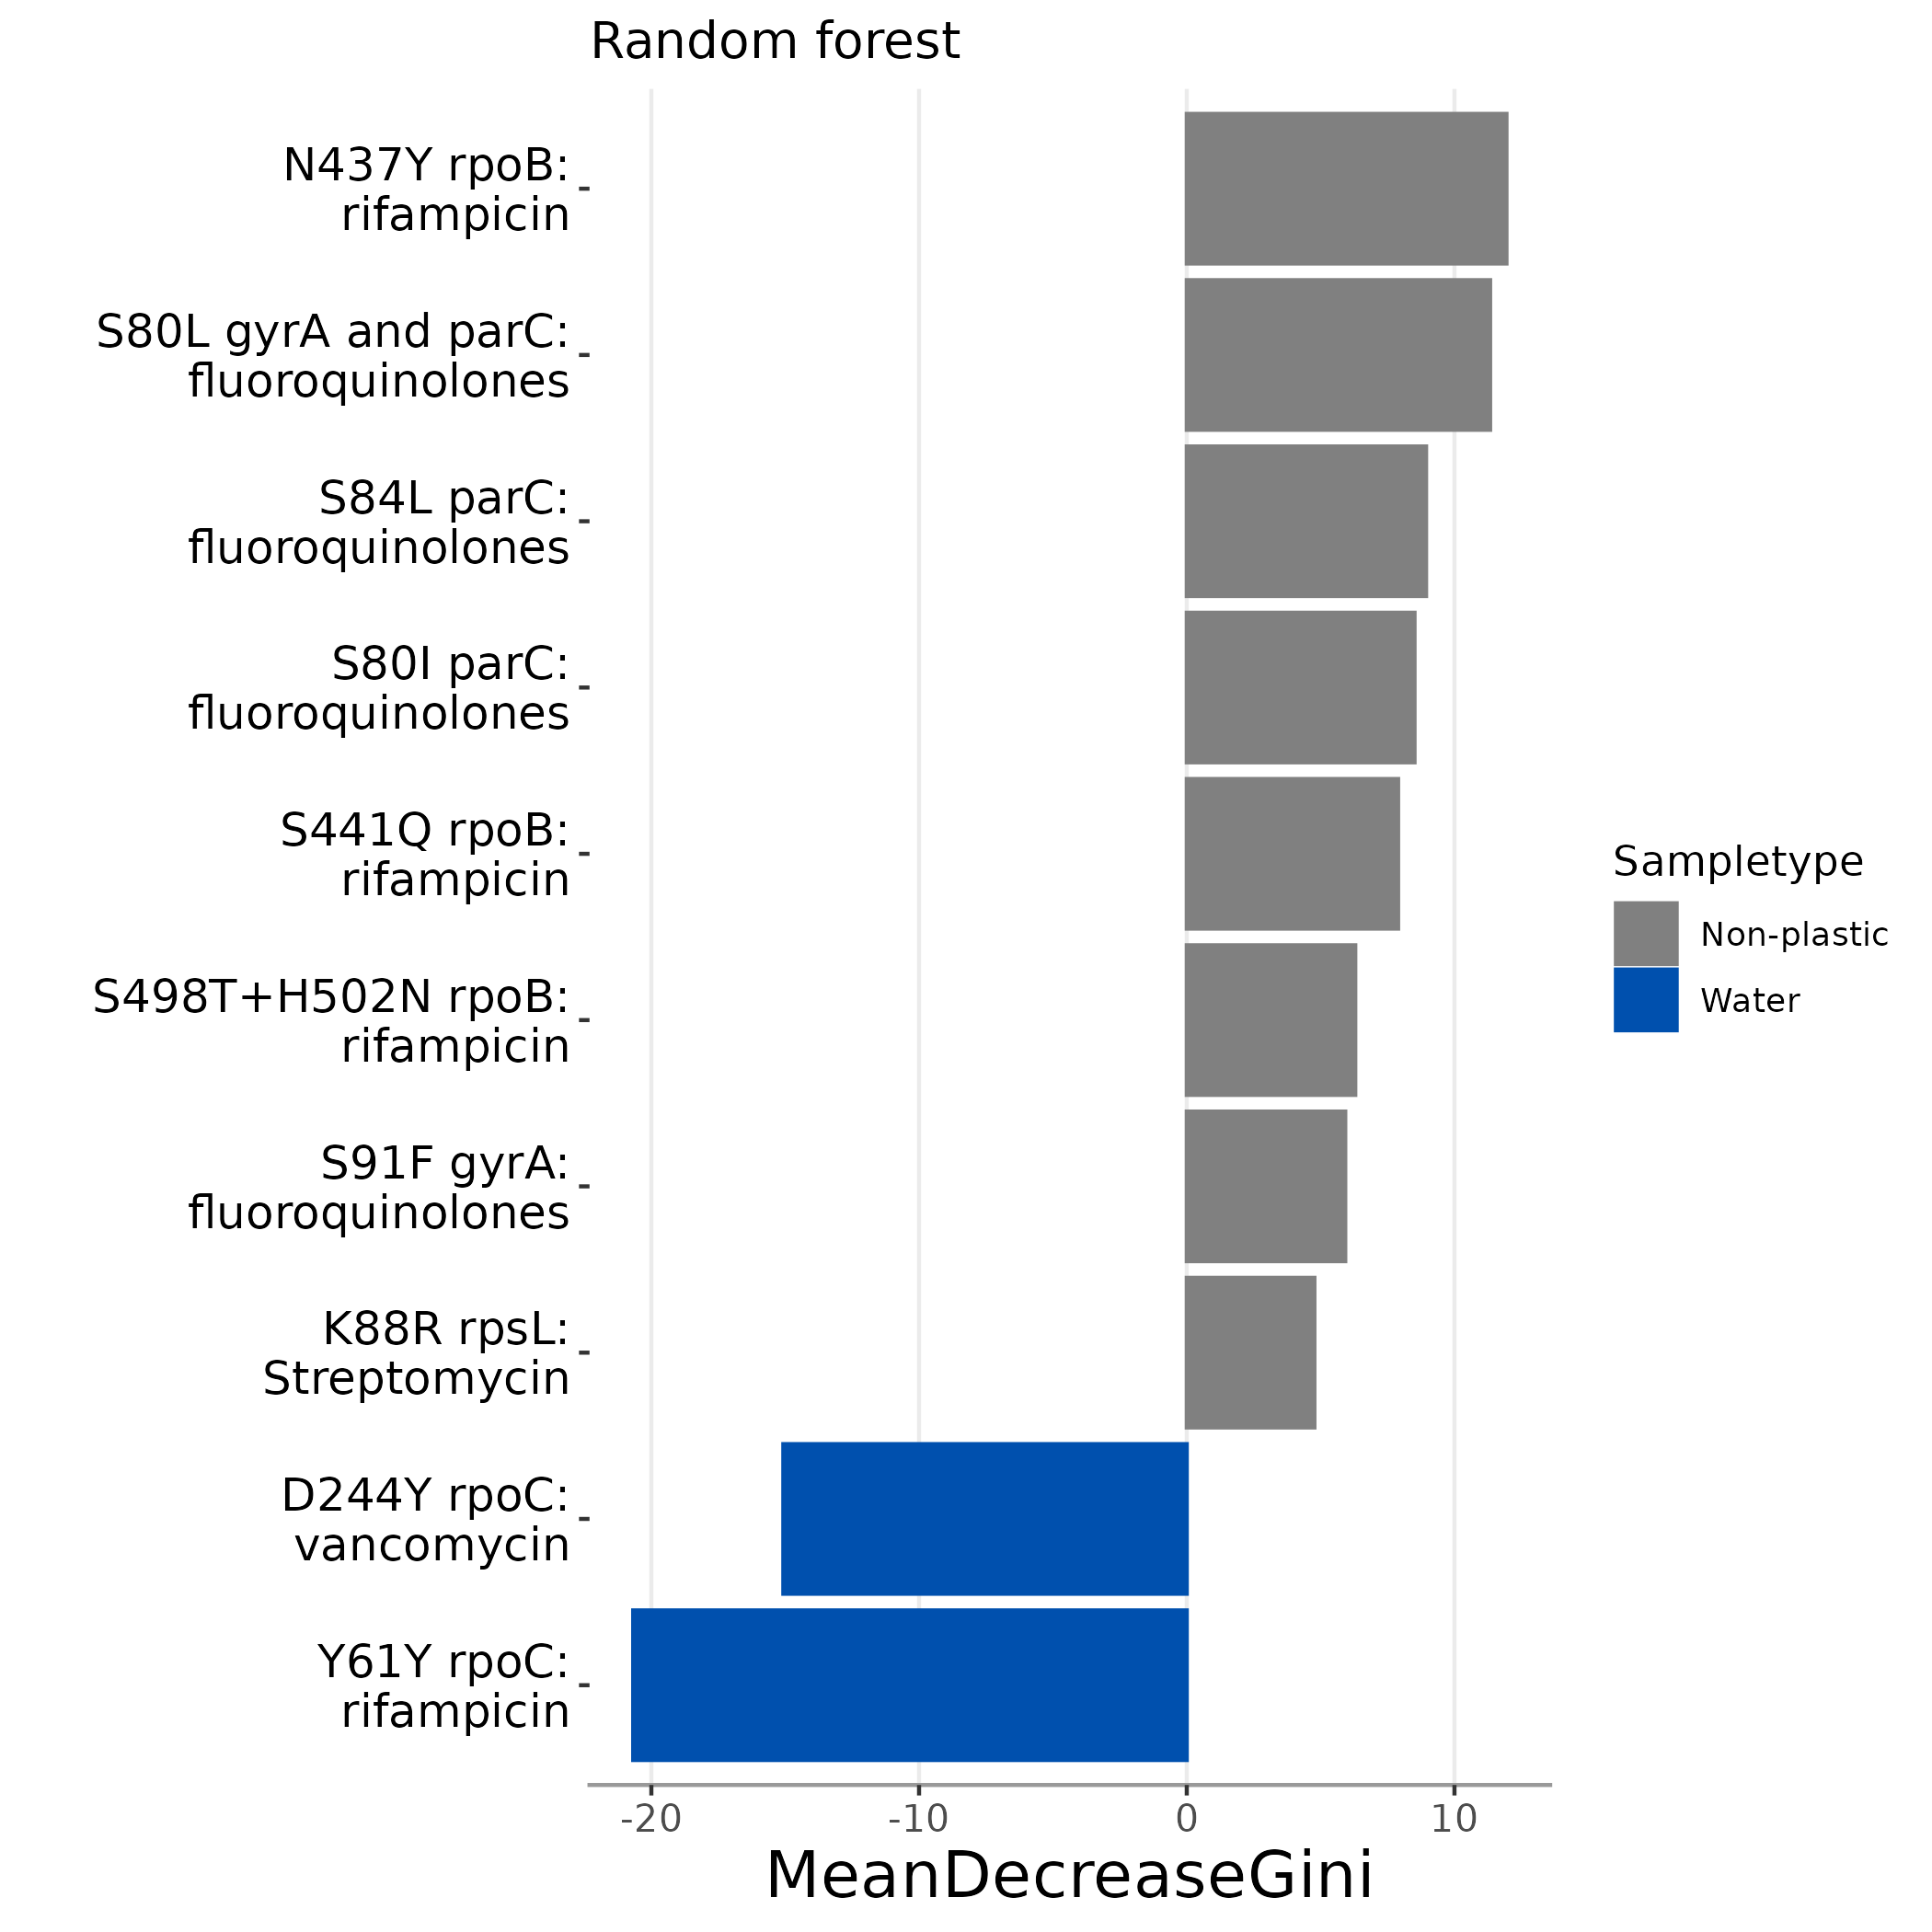
\includegraphics[width=0.5\textwidth]{figure/relative_forest_sampletype_snps_bar.png}}
    \subfloat[\label{snp_sampletype_abund}]{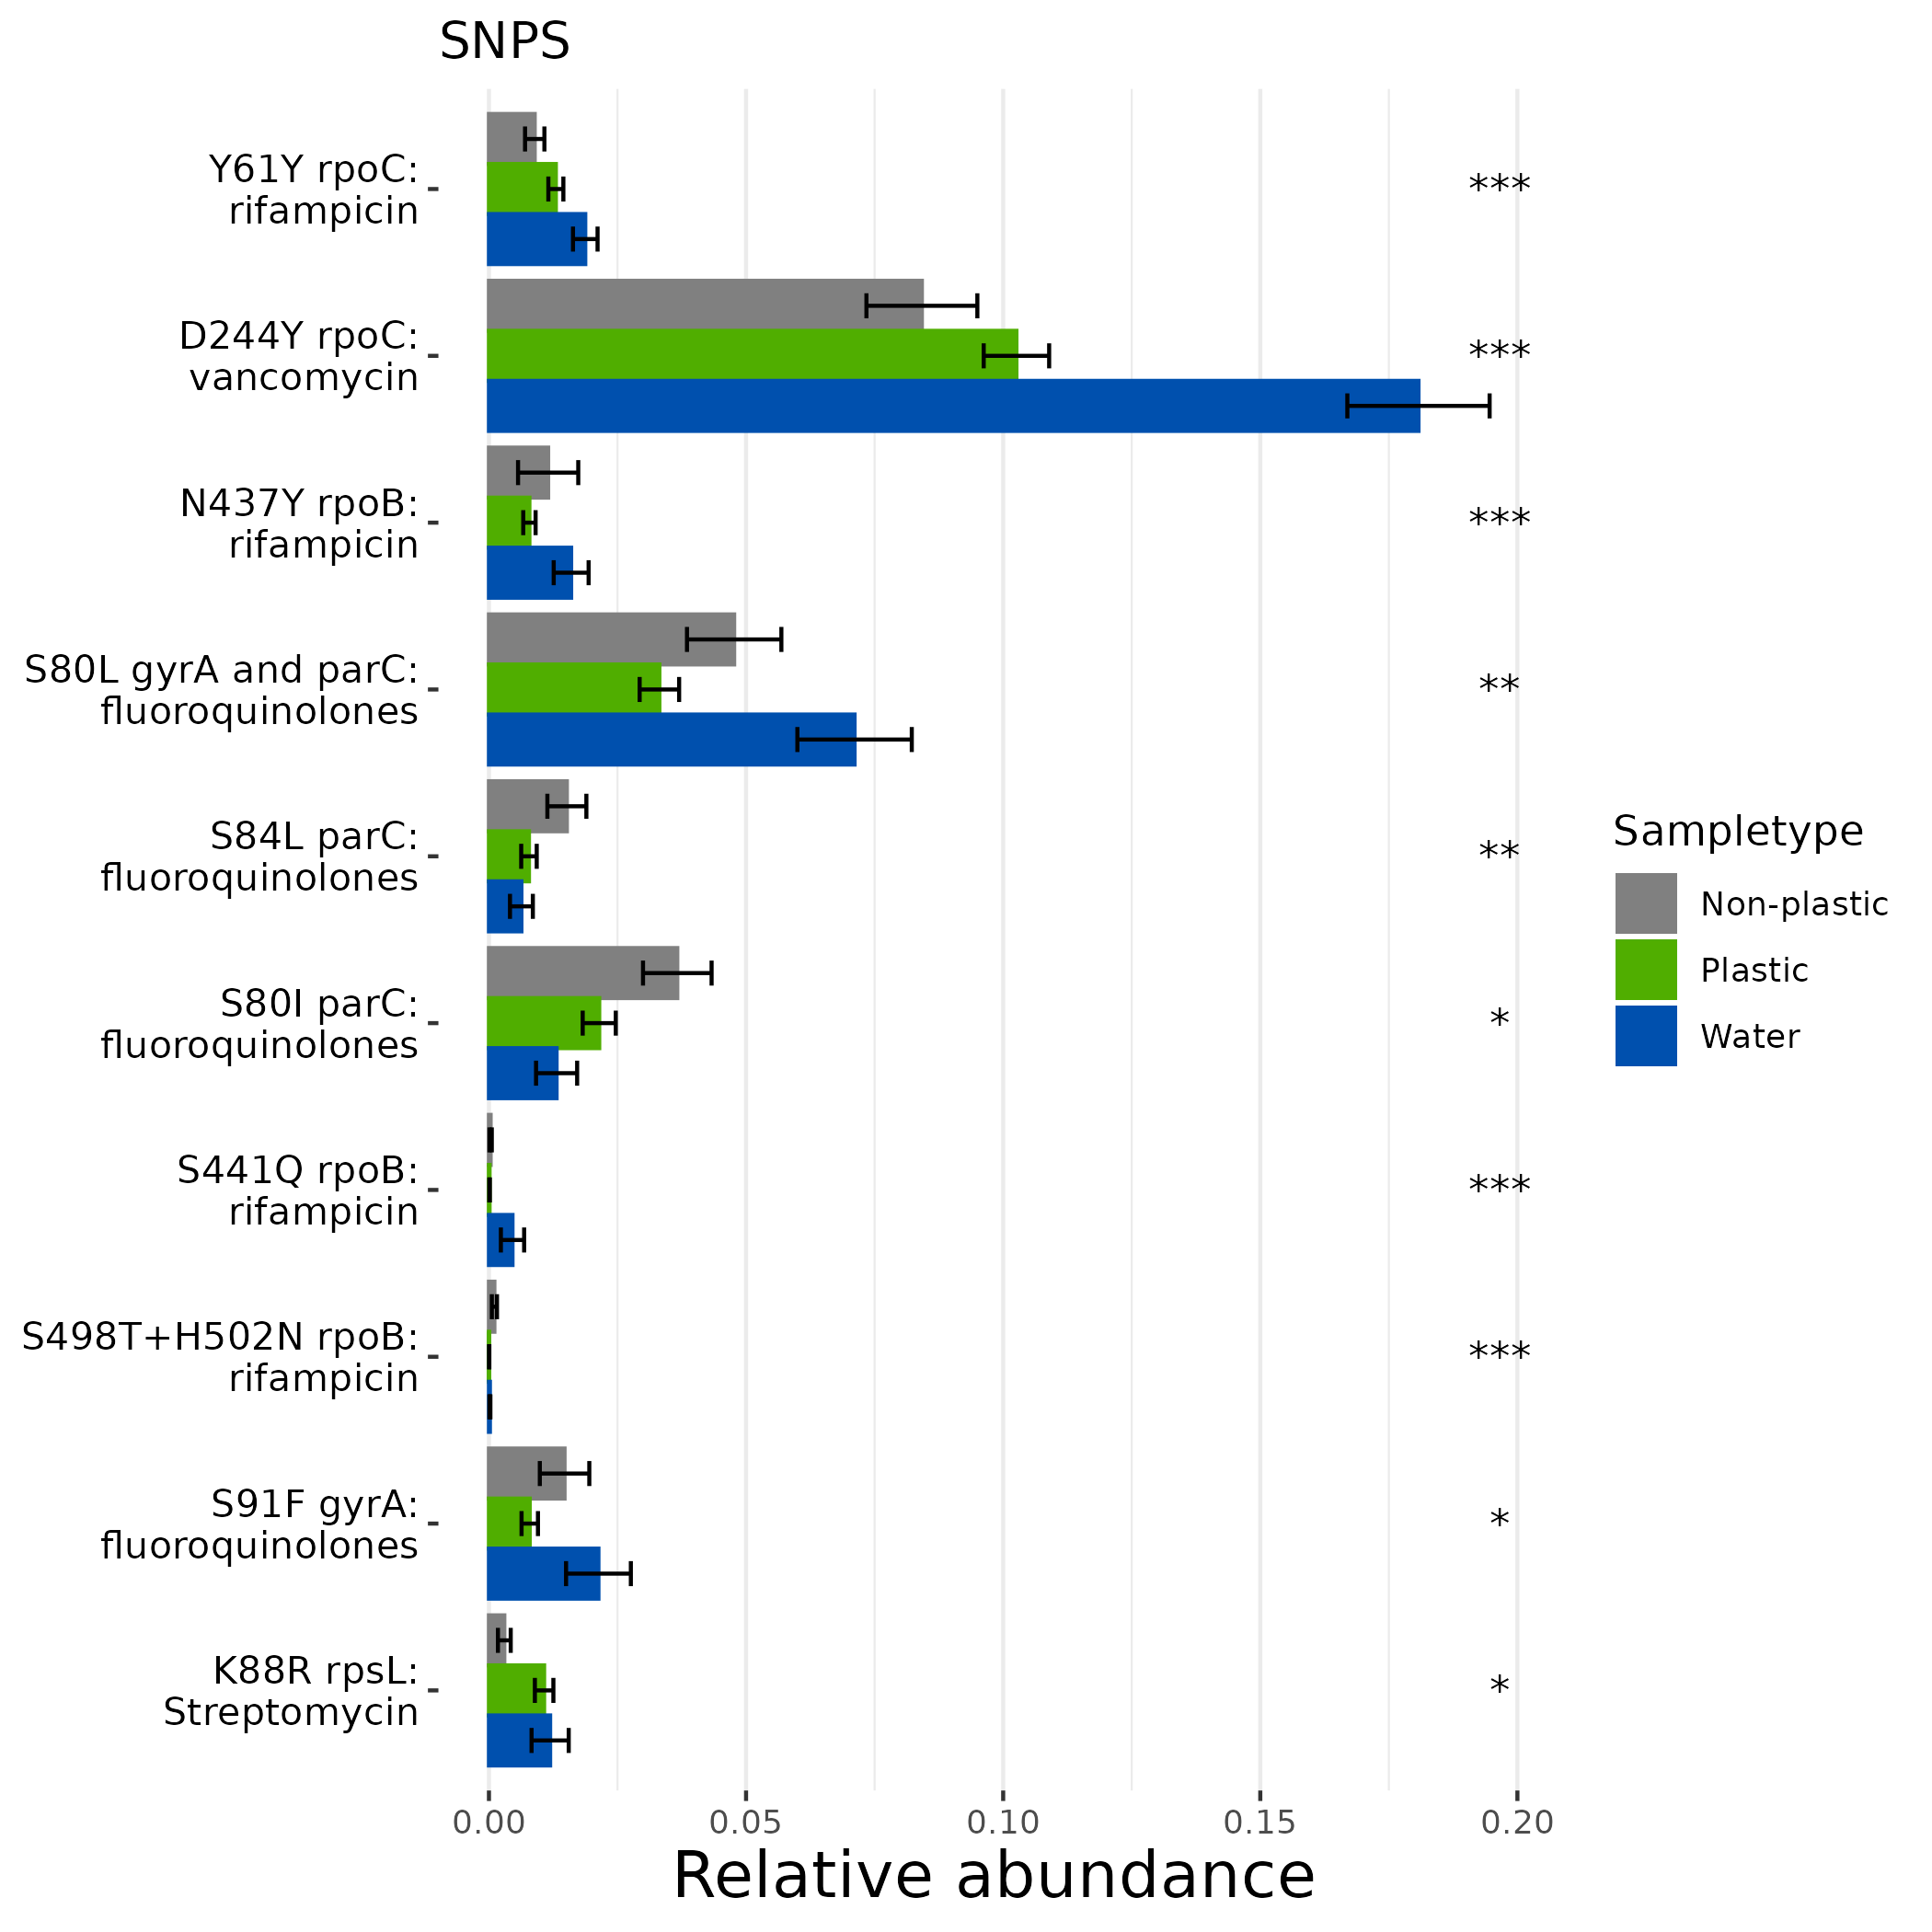
\includegraphics[width=0.5\textwidth]{figure/relative_forest_sampletype_snps_abund.png}}
    \caption{(a) Significantly assigned point mutations and Mean Decrease Gini Importance when grouped by sampletype. (b) Relative Abundances of the different point mutations in the sampletypes}
    \label{snps_sampletype}
\end{figure}

When instead the different substrates is used as the grouping variable in the random forest analysis, the mutations with the highest mean decrease Gini importance are not the same, however many of the genes and the resistances they confer are. These include parC (fluoroquinolones), rpoB (rifampicin), rpoC (rifampicin or vancomycin), gyrB (aminocoumarin), and are shown in figure \ref{snp_substrate_bar}. The mutations in EF-Tu, which confer resistance to pulvomycin, are not present in the previous plot, and may be used to identify ceramic as a substrate. Note however that there are only three ceramic samples in this study, which may skew the results.
%\{note however that there are only 3 ceramic samples used in this study, which may skew the results.}

\begin{figure}[h!]
    \centering
    \subfloat[caption1.\label{snp_substrate_bar}]{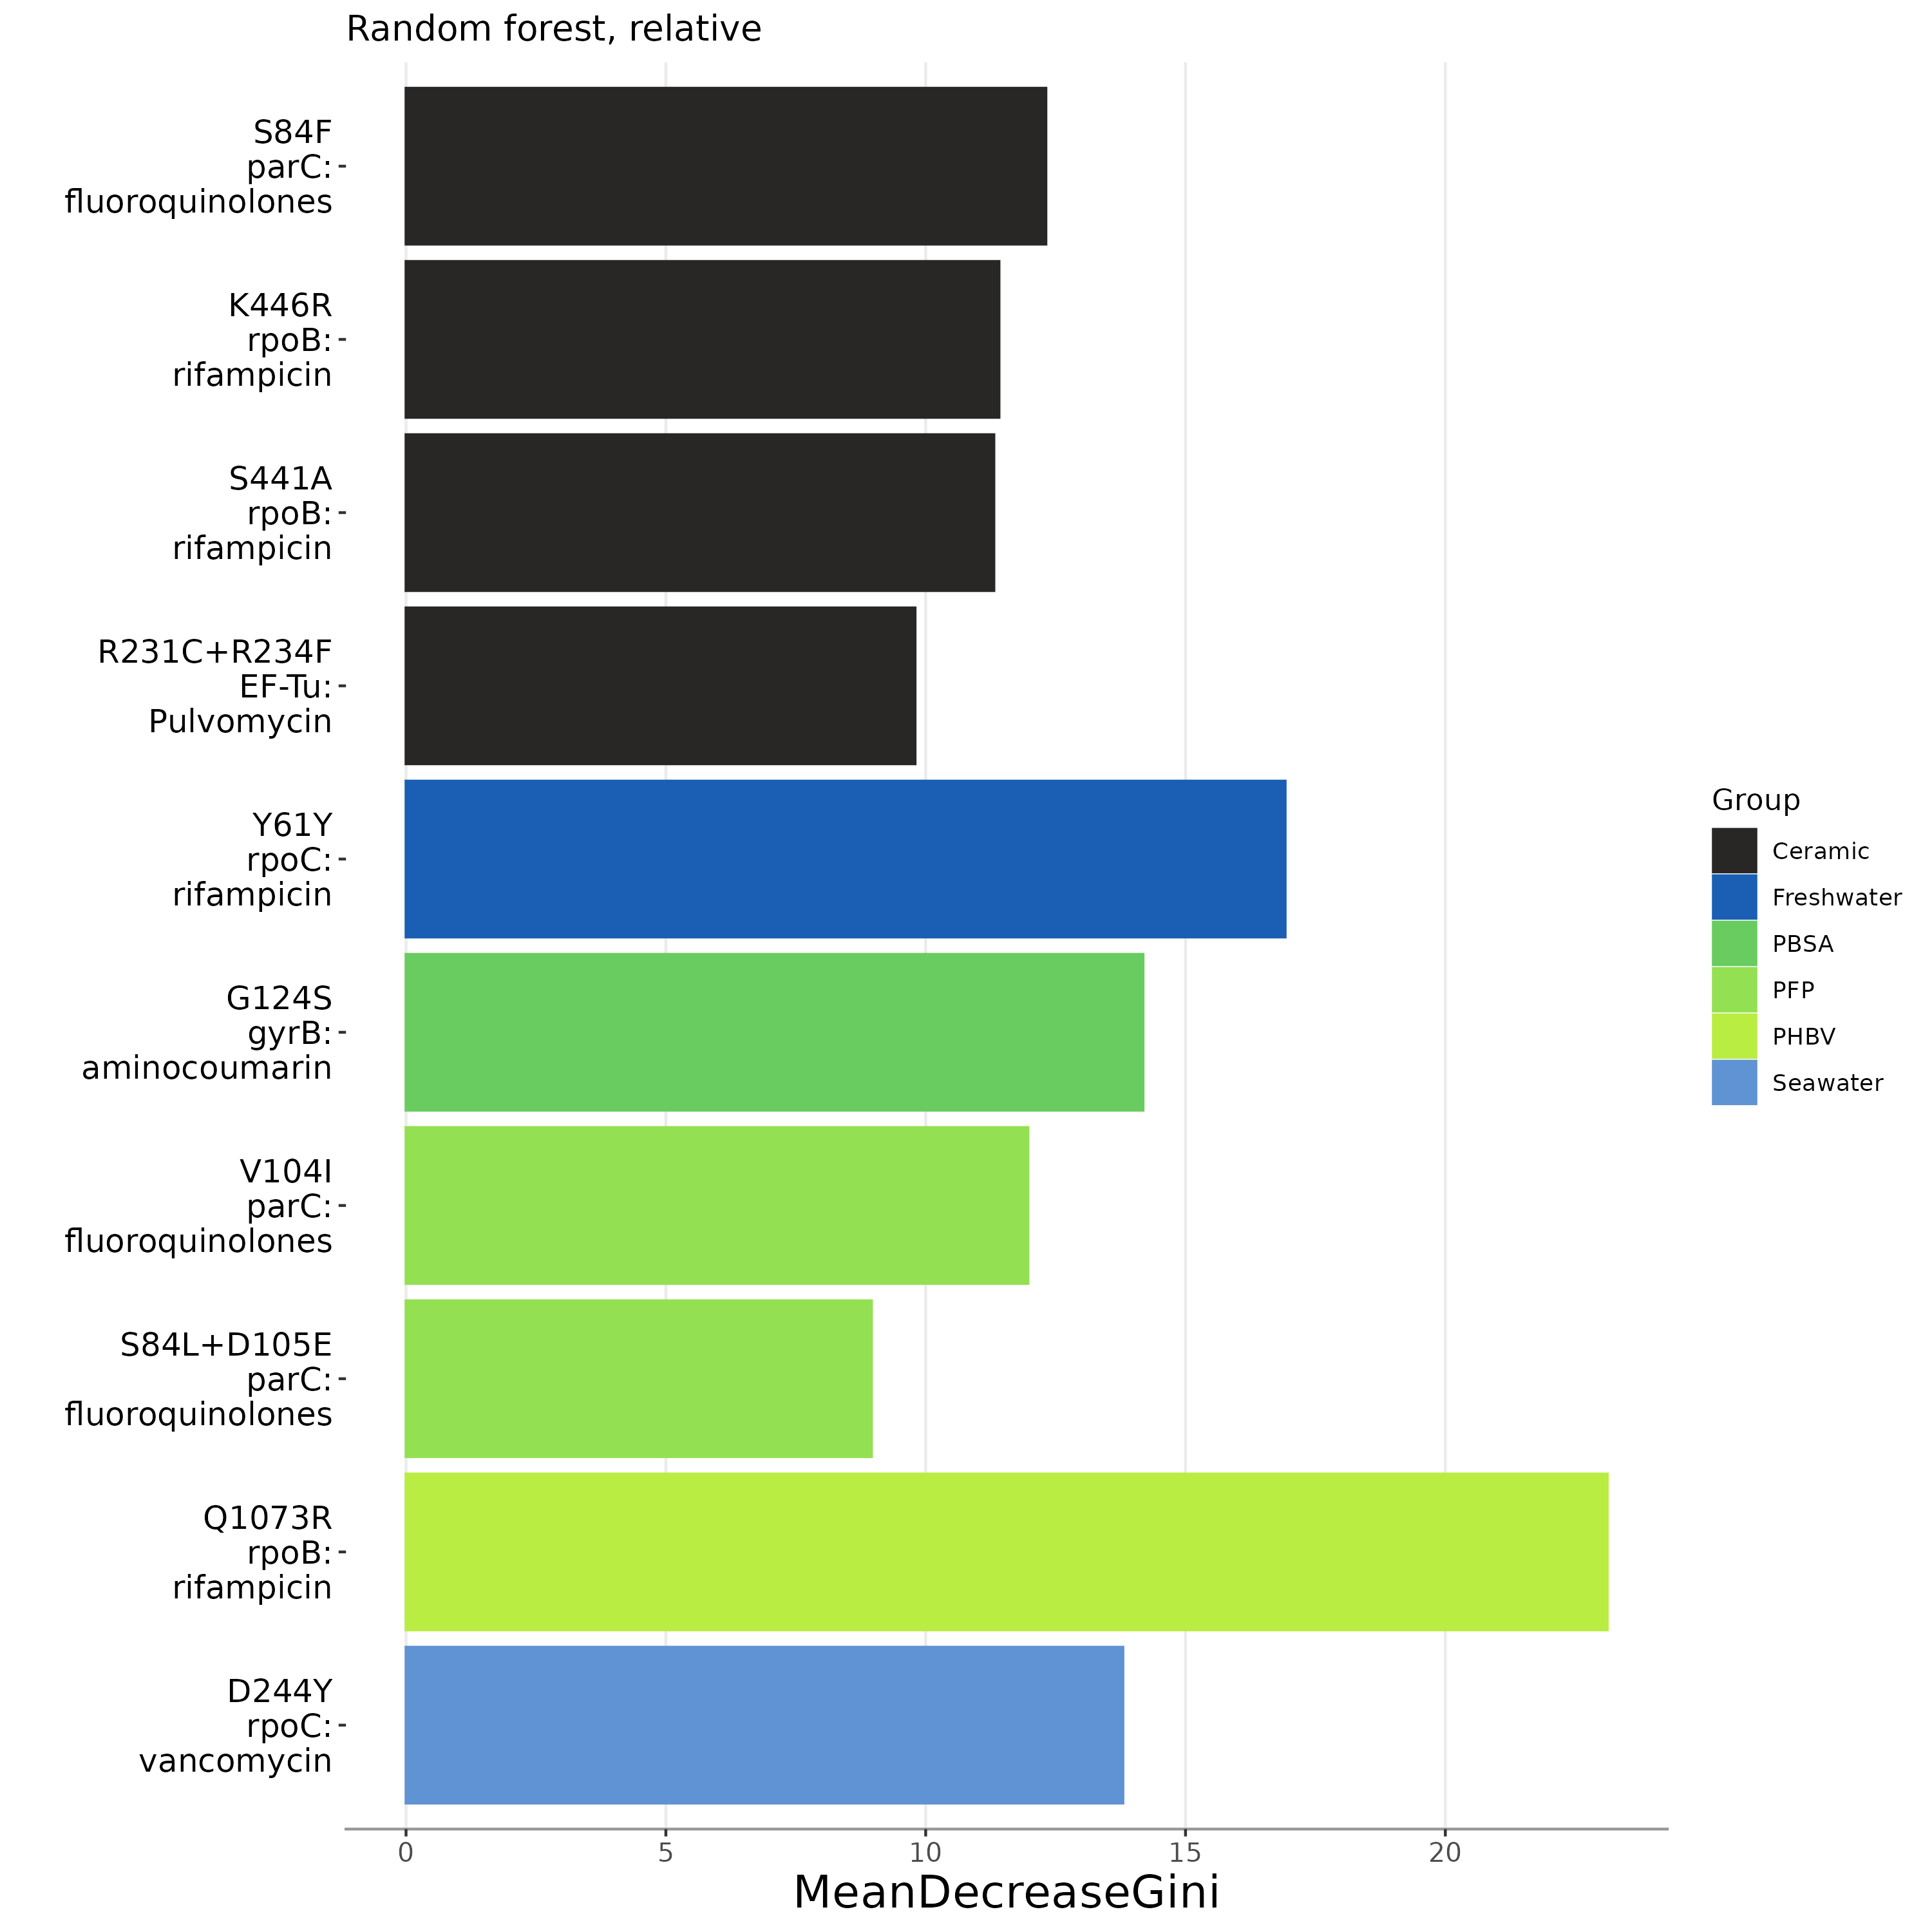
\includegraphics[width=0.5\textwidth]{figure/relative_forest_substrate_snps_bar.png}}
    \subfloat[caption2.\label{snp_substrate_abund}]{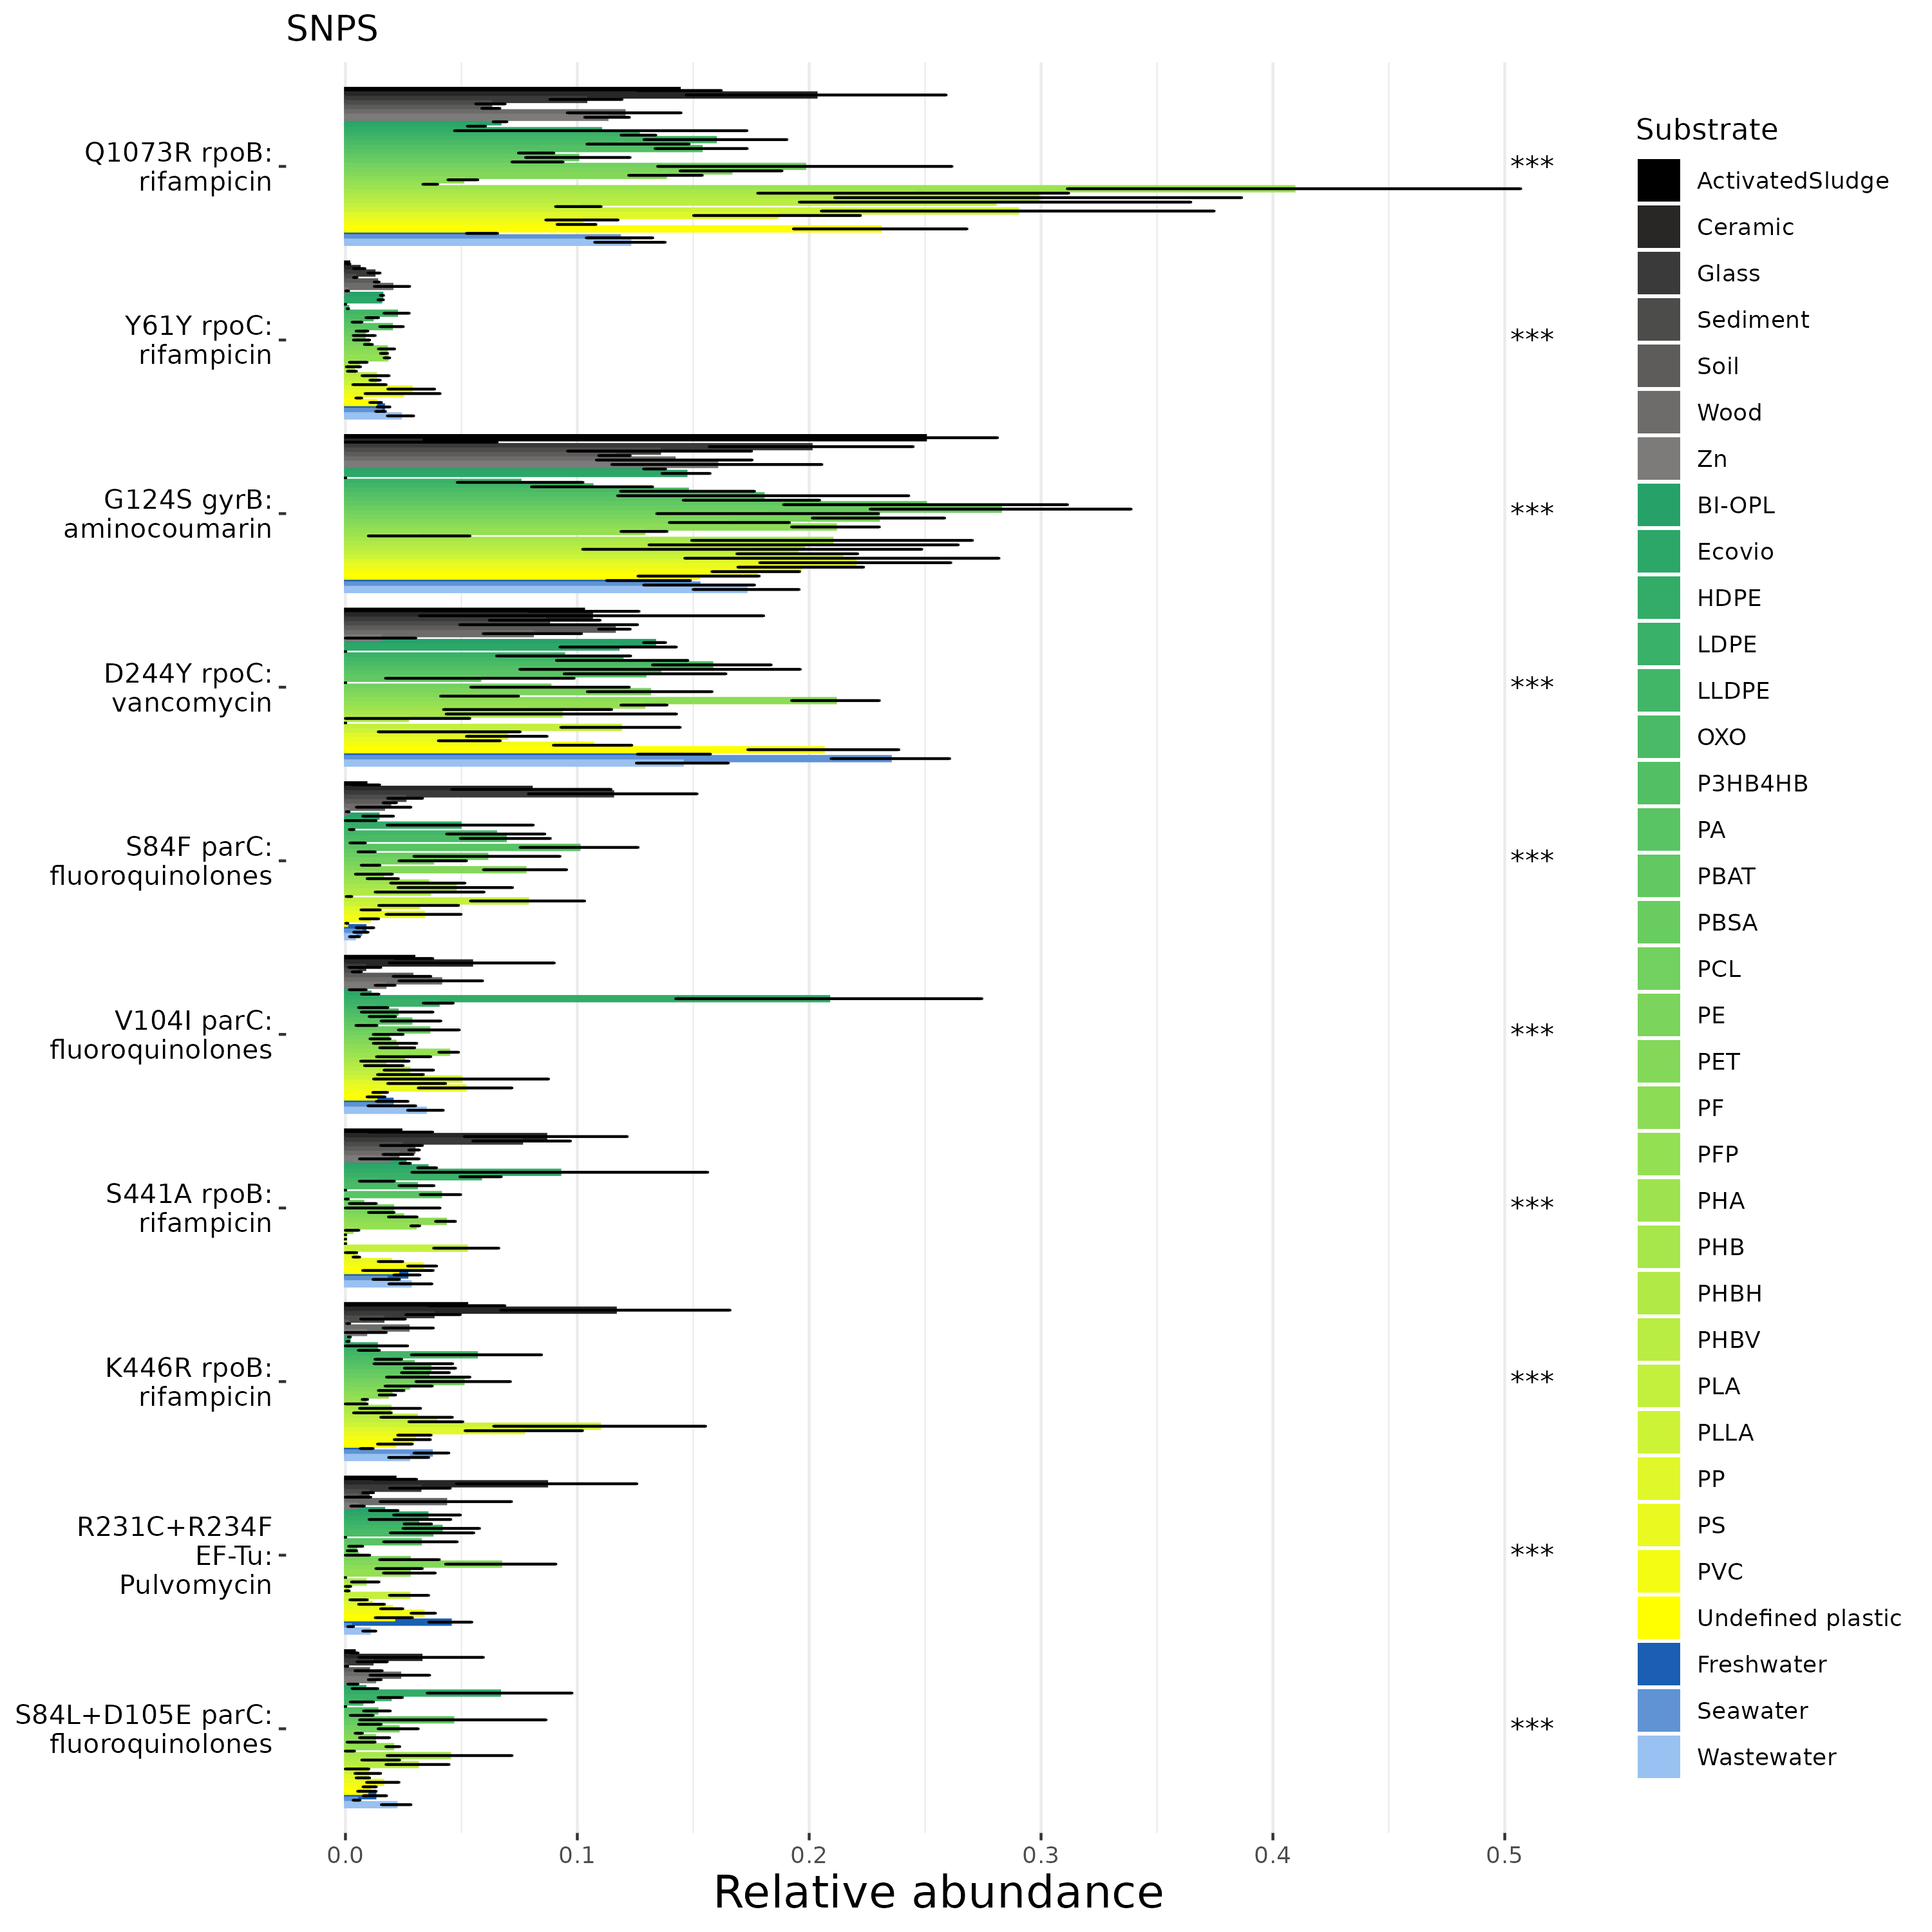
\includegraphics[width=0.5\textwidth]{figure/relative_forest_substrate_snps_abund.png}}
    \caption{(a) Significantly assigned point mutations and Mean Decrease Gini Importance when grouped by substrate. (b) Relative Abundances of the different point mutations in the substrates}
    \label{snps_substrate}
\end{figure}

\section{Taxonomic Composition}
%TODO Show this for the sake of it?
The taxonomic abundance of all samples is shown in figure \ref{tax_plot}. The plot show the taxonomic composition at the phylum level, and is divided by ecosystem type and sampletype. Only the eight most abundant phyla has been included, where the rest has been grouped into "Others".
%The ecosystem type is the environment in which the sample was taken, regardless of the sampletype. For example, some of the samples were taken in the Pacific Ocean, and there both plastic substrates and seawater substrates were analysed.
%The figure shows that the largest difference is between the different ecosystems, but that sampletype also matters.\{Very unsure of how to analuze these plots, since we lack statistics for them.}
The most abundant phyla in all ecosystems are \emph{Proteobacteria}, except in the wastewater samples where SAR is most abundant in most of the samples.
Other abundant phyla are \emph{Archaeplastida} in the PE samples from the Ocean ecosystem, see \ref{tax_plot_substrate_flip}, \emph{Amorphea} in the Undefined palstic samples and in PVC from wastewater. The soil and sediment samples contain a large proportion of Others, into which the phyla not part of the eight most abundant ones are grouped. 

%wastewater: Archaeplastida (Some ocean plastic samples, the PE ones)
%Plastic and wastewater: Amorphea (plastic: undefined, from great pacific garbage patch; wastewater: PVC)
%Soil and sediment: >50\% others

%there are differences between the different ecosystems, but that there is relatively small differences between the different sampletypes and substrates. 

%Figure \ref{tax_plot_substrate} show the same plot, but this time also divided by substrate.\{Which of these should be present? Could turn the whole plot 90° on the page to be easier to read? see fig \ref{tax_plot_substrate_flip}}

\begin{figure}[h]
    \centering
    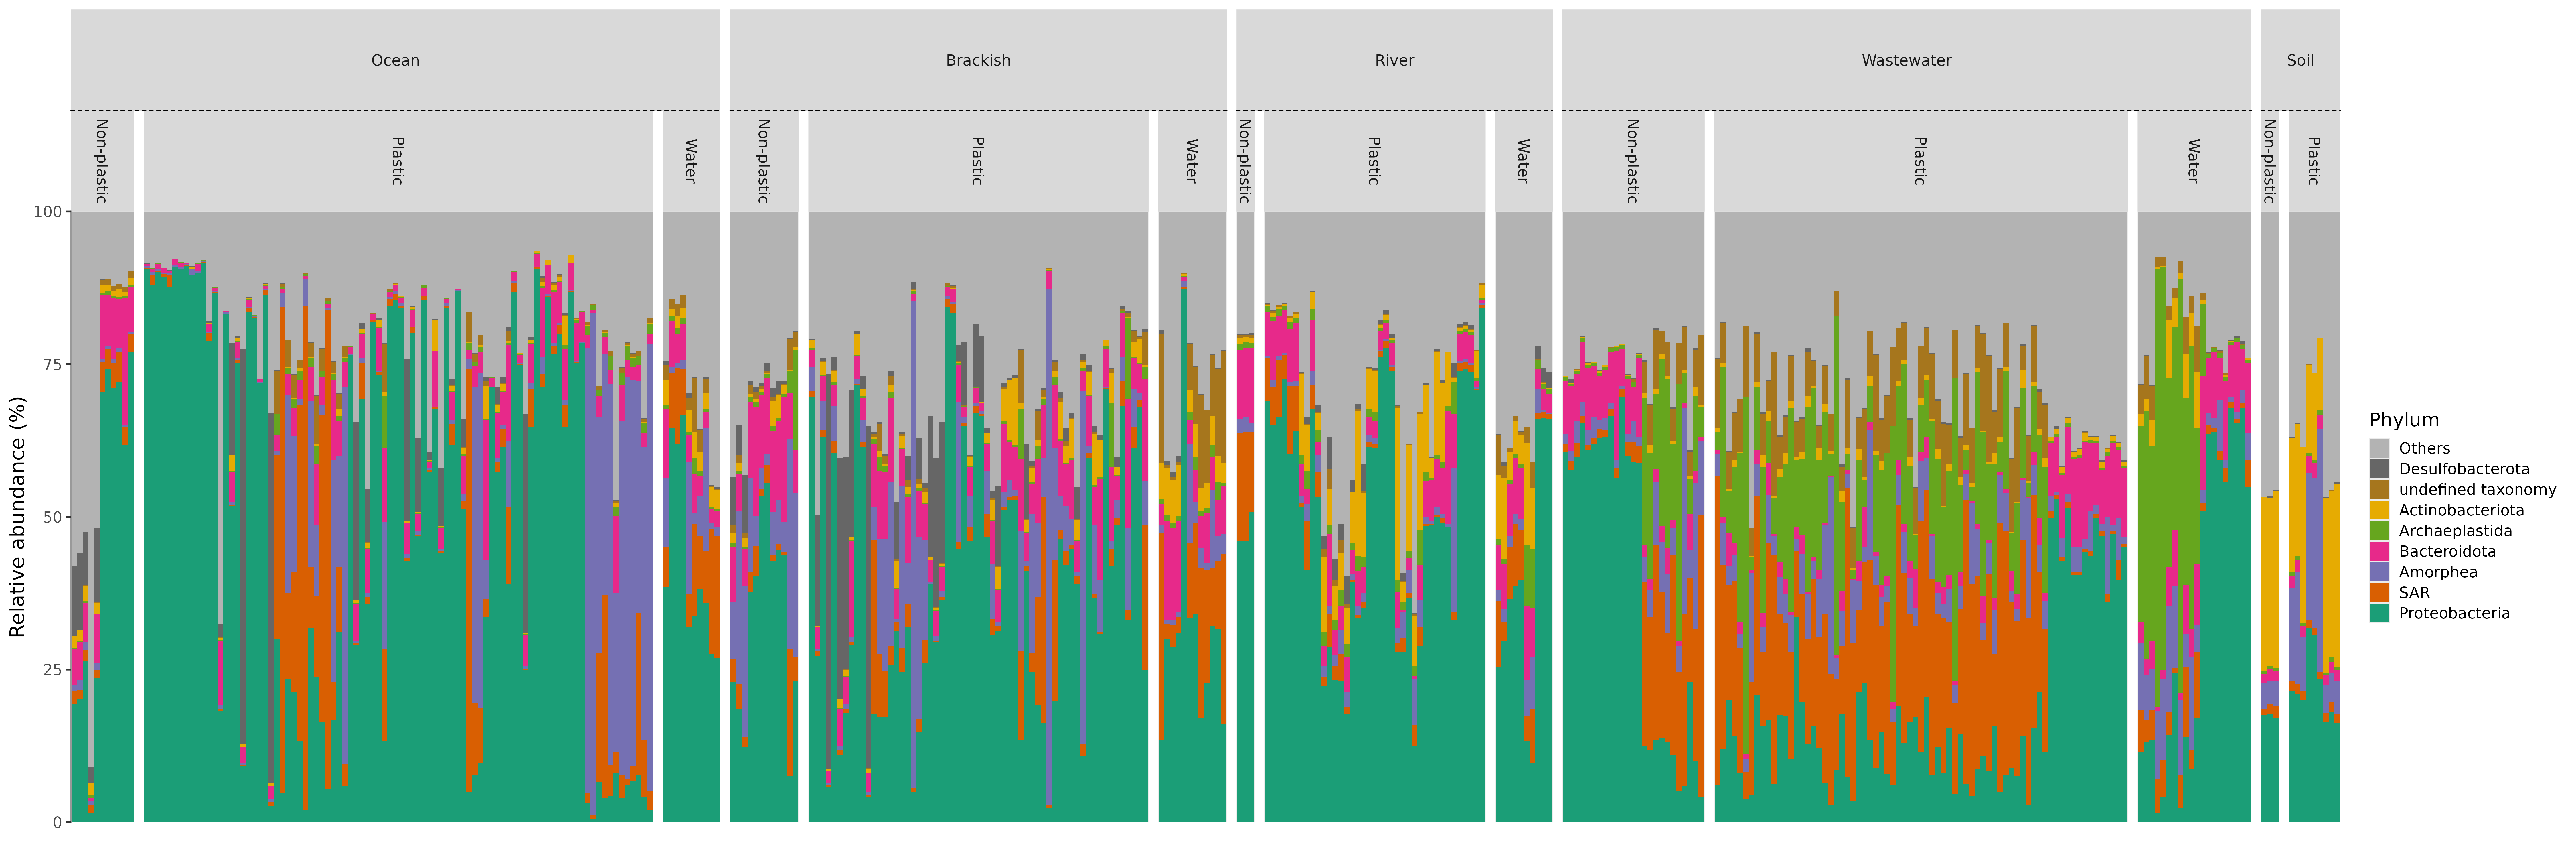
\includegraphics[width = 0.9\textheight, angle = 90]{figure/tax_phylum_ecosystem_sampletype.png}
    \caption{Taxonomic composition for all samples showing the top 8 phyla, divided by ecosystem type and sampletype}
    \label{tax_plot}
\end{figure}












